%
% Copyright (c) 2006 XenSource, Inc.
%
% Permission is granted to copy, distribute and/or modify this document under
% the terms of the GNU Free Documentation License, Version 1.2 or any later
% version published by the Free Software Foundation; with no Invariant
% Sections, no Front-Cover Texts and no Back-Cover Texts.  A copy of the
% license is included in the section entitled
% "GNU Free Documentation License" or the file fdl.tex.
%
% Authors: Ewan Mellor, Richard Sharp, Dave Scott, Jon Harrop.
%

\documentclass{report}

\usepackage{a4wide}
\usepackage{graphics}
\usepackage{longtable}
\usepackage{fancyhdr}

\setlength\topskip{0cm}
\setlength\topmargin{0cm}
\setlength\oddsidemargin{0cm}
\setlength\evensidemargin{0cm}
\setlength\parindent{0pt}

%% Parameters for coversheet:
%
% Copyright (c) 2006-2007 XenSource, Inc.
%
% Permission is granted to copy, distribute and/or modify this document under
% the terms of the GNU Free Documentation License, Version 1.2 or any later
% version published by the Free Software Foundation; with no Invariant
% Sections, no Front-Cover Texts and no Back-Cover Texts.  A copy of the
% license is included in the section entitled
% "GNU Free Documentation License" or the file fdl.tex.
%
% Authors: Ewan Mellor, Richard Sharp, Dave Scott, Jon Harrop.
%

%% Document title
\newcommand{\doctitle}{Xen Management API}

\newcommand{\coversheetlogo}{xen.eps}

%% Document date
\newcommand{\datestring}{11th February 2008}

\newcommand{\releasestatement}{Stable Release}

%% Document revision
\newcommand{\revstring}{API Revision 1.0.5}

%% Document authors
\newcommand{\docauthors}{
Ewan Mellor: & {\tt ewan@xensource.com} \\
Richard Sharp: & {\tt richard.sharp@xensource.com} \\
David Scott: & {\tt david.scott@xensource.com}}
\newcommand{\legalnotice}{Copyright \copyright{} 2006-2007 XenSource, Inc.\\ \\
Permission is granted to copy, distribute and/or modify this document under
the terms of the GNU Free Documentation License, Version 1.2 or any later
version published by the Free Software Foundation; with no Invariant Sections,
no Front-Cover Texts and no Back-Cover Texts.  A copy of the license is
included in the section entitled "GNU Free Documentation License".
}


\begin{document}

% The coversheet itself
%
% Copyright (c) 2006 XenSource, Inc.
%
% Permission is granted to copy, distribute and/or modify this document under
% the terms of the GNU Free Documentation License, Version 1.2 or any later
% version published by the Free Software Foundation; with no Invariant
% Sections, no Front-Cover Texts and no Back-Cover Texts.  A copy of the
% license is included in the section entitled
% "GNU Free Documentation License" or the file fdl.tex.
%
% Authors: Ewan Mellor, Richard Sharp, Dave Scott, Jon Harrop.
%

\pagestyle{empty}

\doctitle{} \hfill \revstring{}

\vspace{1cm}

\begin{center}
\resizebox{8cm}{!}{\includegraphics{\coversheetlogo}}

\vspace{3cm}

\begin{Huge}
  \doctitle{}
\end{Huge}

\vspace{1cm}
\begin{Large}
Version: \revstring{}\\
Date: \datestring{}
\\
\releasestatement{}

\vspace{1cm}
\begin{tabular}{rl}
\docauthors{}
\end{tabular}

\end{Large}
\end{center}

\vfill

\noindent
\legalnotice{}

\newpage
\pagestyle{fancy}

% ... and off we go!

\chapter{Introduction}

This document contains a description of the Xen Management API---an interface for
remotely configuring and controlling virtualised guests running on a
Xen-enabled host. 

~

{\bf \large This document is an early draft for discussion purposes only.}

~

%
% Copyright (c) 2006-2007 XenSource, Inc.
%
% Permission is granted to copy, distribute and/or modify this document under
% the terms of the GNU Free Documentation License, Version 1.2 or any later
% version published by the Free Software Foundation; with no Invariant
% Sections, no Front-Cover Texts and no Back-Cover Texts.  A copy of the
% license is included in the section entitled
% "GNU Free Documentation License" or the file fdl.tex.
%
% Authors: Ewan Mellor, Richard Sharp, Dave Scott, Jon Harrop.
%

The API is presented here as a set of Remote Procedure Calls, with a wire
format based upon XML-RPC. No specific language bindings are prescribed,
although examples will be given in the python programming language.
 
Although we adopt some terminology from object-oriented programming, 
future client language bindings may or may not be object oriented.
The API reference uses the terminology {\em classes\/} and {\em objects\/}.
For our purposes a {\em class\/} is simply a hierarchical namespace;
an {\em object\/} is an instance of a class with its fields set to
specific values. Objects are persistent and exist on the server-side.
Clients may obtain opaque references to these server-side objects and then
access their fields via get/set RPCs.

%In each class there is a $\mathit{uid}$ field that assigns an indentifier
%to each object. This $\mathit{uid}$ serves as an object reference
%on both client- and server-side, and is often included as an argument in
%RPC messages.

For each class we specify a list of
fields along with their {\em types\/} and {\em qualifiers\/}.  A
qualifier is one of:
\begin{itemize}
  \item $\mathit{RO}_\mathit{run}$: the field is Read
Only. Furthermore, its value is automatically computed at runtime.
For example: current CPU load and disk IO throughput.
  \item $\mathit{RO}_\mathit{ins}$: the field must be manually set
when a new object is created, but is then Read Only for
the duration of the object's life.
For example, the maximum memory addressable by a guest is set 
before the guest boots.
  \item $\mathit{RW}$: the field is Read/Write. For example, the name
of a VM.
\end{itemize}

A full list of types is given in Chapter~\ref{api-reference}. However,
there are three types that require explicit mention:
\begin{itemize}
  \item $t~\mathit{Ref}$: signifies a reference to an object
of type $t$.
  \item $t~\mathit{Set}$: signifies a set containing
values of type $t$.
  \item $(t_1, t_2)~\mathit{Map}$: signifies a mapping from values of
type $t_1$ to values of type $t_2$.
\end{itemize}

Note that there are a number of cases where {\em Ref}s are {\em doubly
linked\/}---e.g.\ a VM has a field called {\tt VIFs} of type
$(\mathit{VIF}~\mathit{Ref})~\mathit{Set}$; this field lists
the network interfaces attached to a particular VM. Similarly, the VIF
class has a field called {\tt VM} of type $(\mathit{VM}~{\mathit
Ref})$ which references the VM to which the interface is connected.
These two fields are {\em bound together\/}, in the sense that
creating a new VIF causes the {\tt VIFs} field of the corresponding
VM object to be updated automatically.

The API reference explicitly lists the fields that are
bound together in this way. It also contains a diagram that shows
relationships between classes. In this diagram an edge signifies the
existence of a pair of fields that are bound together, using standard
crows-foot notation to signify the type of relationship (e.g.\
one-many, many-many).

\section{RPCs associated with fields}

Each field, {\tt f}, has an RPC accessor associated with it
that returns {\tt f}'s value:
\begin{itemize}
\item ``{\tt get\_f(Ref x)}'': takes a
{\tt Ref} that refers to an object and returns the value of {\tt f}.
\end{itemize}

Each field, {\tt f}, with attribute
{\em RW} and whose outermost type is {\em Set\/} has the following
additional RPCs associated with it:
\begin{itemize}
\item an ``{\tt add\_to\_f(Ref x, v)}'' RPC adds a new element v to the set\footnote{
%
Since sets cannot contain duplicate values this operation has no action in the case
that {\tt v} was already in the set.
%
};
\item a ``{\tt remove\_from\_f(Ref x, v)}'' RPC removes element {\tt v} from the set;
\end{itemize}

Each field, {\tt f}, with attribute
{\em RW} and whose outermost type is {\em Map\/} has the following
additional RPCs associated with it:
\begin{itemize}
\item an ``{\tt add\_to\_f(Ref x, k, v)}'' RPC adds new pair {\tt (k, v)}
to the mapping stored in {\tt f} in object {\tt x}. Adding a new pair for duplicate
key, {\tt k}, overwrites any previous mapping for {\tt k}.
\item a ``{\tt remove\_from\_f(Ref x, k)}'' RPC removes the pair with key {\tt k}
from the mapping stored in {\tt f} in object {\tt x}.
\end{itemize}

Each field whose outermost type is neither {\em Set\/} nor {\em Map\/}, 
but whose attribute is {\em RW} has an RPC acessor associated with it
that sets its value:
\begin{itemize}
\item For {\em RW\/} ({\em R\/}ead/{\em
W\/}rite), a ``{\tt set\_f(Ref x, v)}'' RPC function is also provided.
This sets field {\tt f} on object {\tt x} to value {\tt v}.
\end{itemize}

\section{RPCs associated with classes}

\begin{itemize}
\item Each class has a {\em constructor\/} RPC named ``{\tt create}'' that
takes as parameters all fields marked {\em RW\/} and
$\mathit{RO}_\mathit{ins}$. The result of this RPC is that a new {\em
persistent\/} object is created on the server-side with the specified field
values.

\item Each class has a {\tt get\_by\_uuid(uuid)} RPC that returns the object
of that class that has the specified {\tt uuid}.

\item Each class that has a {\tt name\_label} field has a
``{\tt get\_by\_name\_label(name)}'' RPC that returns a set of objects of that
class that have the specified {\tt label}.

\item Each class has a ``{\tt destroy(Ref x)}'' RPC that explicitly deletes
the persistent object specified by {\tt x} from the system.  This is a
non-cascading delete -- if the object being removed is referenced by another
object then the {\tt destroy} call will fail.

\end{itemize}

\subsection{Additional RPCs}

As well as the RPCs enumerated above, some classes have additional RPCs
associated with them. For example, the {\tt VM} class has RPCs for cloning,
suspending, starting etc. Such additional RPCs are described explicitly
in the API reference.


%
% Copyright (c) 2006 XenSource, Inc.
%
% Permission is granted to copy, distribute and/or modify this document under
% the terms of the GNU Free Documentation License, Version 1.2 or any later
% version published by the Free Software Foundation; with no Invariant
% Sections, no Front-Cover Texts and no Back-Cover Texts.  A copy of the
% license is included in the section entitled
% "GNU Free Documentation License" or the file fdl.tex.
%
% Authors: Ewan Mellor, Richard Sharp, Dave Scott, Jon Harrop.
%

\section{Wire Protocol for Remote API Calls}

API calls are sent over a network to a Xen-enabled host using
the XML-RPC protocol. In this Section we describe how the
higher-level types used in our API Reference are mapped to
primitive XML-RPC types.

In our API Reference we specify the signatures of API functions in the following
style:
\begin{verbatim}
    (ref_vm Set)   VM.get_all()
\end{verbatim}
This specifies that the function with name {\tt VM.get\_all} takes
no parameters and returns a Set of {\tt ref\_vm}s.
These types are mapped onto XML-RPC types in a straight-forward manner:
\begin{itemize}
  \item Floats, Bools, DateTimes and Strings map directly to the XML-RPC {\tt
  double}, {\tt boolean}, {\tt dateTime.iso8601}, and {\tt string} elements.

  \item all our ``{\tt ref\_}'' types (e.g.\ {\tt ref\_vm} in the above
  example) map to XML-RPC's {\tt String} type.  The string itself is the OSF
  DCE UUID presentation format (as output by {\tt uuidgen}, etc).

  \item ints are all assumed to be 64-bit in our API and are encoded as a
  string of decimal digits (rather than using XML-RPC's built-in 32-bit {\tt
  i4} type).

  \item values of enum types are encoded as strings. For example, a value of
  {\tt destroy} of type {\tt on\_normal\_exit}, would be conveyed as:
  \begin{verbatim}
    <value><string>destroy</string></value>
  \end{verbatim}

  \item for all our types, {\tt t}, our type {\tt t Set} simply maps to
  XML-RPC's {\tt Array} type, so for example a value of type {\tt cpu\_feature
  Set} would be transmitted like this:

  \begin{verbatim}
<array>
  <data>
    <value><string>CX8</string></value>
    <value><string>PSE36</string></value>
    <value><string>FPU</string></value>
  </data>
</array> 
  \end{verbatim}

  \item for types {\tt k} and {\tt v}, our type {\tt (k, v) Map} maps onto an
  XML-RPC struct, with the key as the name of the struct.  Note that the {\tt
  (k, v) Map} type is only valid when {\tt k} is a {\tt String}, {\tt Ref}, or
  {\tt Int}, and in each case the keys of the maps are stringified as
  above. For example, the {\tt (String, double) Map} containing a the mappings
  Mike $\rightarrow$ 2.3 and John $\rightarrow$ 1.2 would be represented as:

  \begin{verbatim}
<value>
  <struct>
    <member>
      <name>Mike</name>
      <value><double>2.3</double></value>
    </member>
    <member>
      <name>John</name>
      <value><double>1.2</double></value>
    </member>
  </struct>
</value>
  \end{verbatim}

  \item our {\tt Void} type is transmitted as an empty string.

\end{itemize}

\subsection{Return Values/Status Codes}
\label{synchronous-result}

The return value of an RPC call is an XML-RPC {\tt Struct}.

\begin{itemize}
\item The first element of the struct is named {\tt Status}; it
contains a string value indicating whether the result of the call was
a ``{\tt Success}'' or a ``{\tt Failure}''.
\end{itemize}

If {\tt Status} was set to {\tt Success} then the Struct contains a second
element named {\tt Value}:
\begin{itemize}
\item The element of the struct named {\tt Value} contains the function's return value.
\end{itemize}

In the case where {\tt Status} is set to {\tt Failure} then
the struct contains a second element named {\tt ErrorDescription}:
\begin{itemize}
\item The element of the struct named {\tt ErrorDescription} contains
an array of string values. The first element of the array is an XML-RPC 32-bit {\tt i4} and represents an error code;
the remainder of the array are strings representing error parameters relating to that code.
\end{itemize}

For example, an XML-RPC return value from the {\tt Host.ListAllVMs} function above
may look like this:
\begin{verbatim}
    <struct>
       <member>
         <name>Status</name>
         <value>Success</value>
       </member>
       <member>
          <name>Value</name>
          <value>
            <array>
               <data>
                 <value>vm-id-1</value>
                 <value>vm-id-2</value>
                 <value>vm-id-3</value>
               </data>
            </array>
         </value>
       </member>
    </struct>
\end{verbatim}

\section{Making XML-RPC Calls}

\subsection{Transport Layer}

We ought to support at least
\begin{itemize}
\item HTTP/S for remote administration
\item HTTP over Unix domain sockets for local administration
\end{itemize}

\subsection{Session Layer}

The XML-RPC interface is session-based; before you can make arbitrary RPC calls
you must login and initiate a session. For example:
\begin{verbatim}
   session_id    Session.login_with_password(string uname, string pwd)
\end{verbatim}
Where {\tt uname} and {\tt password} refer to your username and password
respectively, as defined by the Xen administrator.
The {\tt session\_id} returned by {\tt Session.Login} is passed to subequent
RPC calls as an authentication token.

A session can be terminated with the {\tt Session.Logout} function:
\begin{verbatim}
   void          Session.Logout(session_id session)
\end{verbatim}

\subsection{Synchronous and Asynchronous invocation}

Each method call (apart from methods on ``Session'' and ``Task'' objects 
and ``getters'' and ``setters'' derived from fields)
can be made either synchronously or asynchronously.
A synchronous RPC call blocks until the
return value is received; the return value of a synchronous RPC call is
exactly as specified in Section~\ref{synchronous-result}.

Only synchronous API calls are listed explicitly in this document. 
All asynchronous versions are in the special {\tt Async} namespace.
For example, synchronous call {\tt VM.clone(...)}
(described in Chapter~\ref{api-reference})
has an asynchronous counterpart, {\tt
Async.VM.clone(...)}, that is non-blocking.

Instead of returning its result directly, an asynchronous RPC call
returns a {\tt task-id}; this identifier is subsequently used
to track the status of a running asynchronous RPC. Note that an asychronous
call may fail immediately, before a {\tt task-id} has even been created---to
represent this eventuality, the returned {\tt task-id}
is wrapped in an XML-RPC struct with a {\tt Status}, {\tt ErrorDescription} and
{\tt Value} fields, exactly as specified in Section~\ref{synchronous-result}.

The {\tt task-id} is provided in the {\tt Value} field if {\tt Status} is set to
{\tt Success}.

The RPC call
\begin{verbatim}
    (ref_task Set)   Task.get_all(session_id s)
\end{verbatim} 
returns a set of all task IDs known to the system. The status (including any
returned result and error codes) of these tasks
can then be queried by accessing the fields of the Task object in the usual way. 
Note that, in order to get a consistent snapshot of a task's state, it is advisable to call the ``get\_record'' function.

\section{Example interactive session}

This section describes how an interactive session might look, using the python
XML-RPC client library. 

First, initialise python and import the library {\tt xmlrpclib}:

\begin{verbatim}
\$ python2.4
...
>>> import xmlrpclib
\end{verbatim}

Create a python object referencing the remote server:

\begin{verbatim}
>>> xen = xmlrpclib.Server("http://test:4464")
\end{verbatim}

Acquire a session token by logging in with a username and password (error-handling ommitted for brevity; the session token is pointed to by the key {\tt 'Value'} in the returned dictionary)

\begin{verbatim}
>>> session = xen.Session.do_login_with_password("user", "passwd")['Value']
\end{verbatim}

When serialised, this call looks like the following:

\begin{verbatim}
<?xml version='1.0'?>
<methodCall>
  <methodName>Session.do_login_with_password</methodName>
  <params>
    <param>
      <value><string>user</string></value>
    </param>
    <param>
      <value><string>passwd</string></value>
    </param>
  </params>
</methodCall>
\end{verbatim}

Next, the user may acquire a list of all the VMs known to the host: (Note the call takes the session token as the only parameter)

\begin{verbatim}
>>> all_vms = xen.VM.do_list(session)['Value']
>>> all_vms
['b7b92d9e-d442-4710-92a5-ab039fd7d89b', '23e1e837-abbf-4675-b077-d4007989b0cc',
  '2045dbc0-0734-4eea-9cb2-b8218c6b5bf2', '3202ae18-a046-4c32-9fda-e32e9631866e']
\end{verbatim}

Note the VM references are internally UUIDs. Once a reference to a VM has been acquired a lifecycle operation may be invoked:

\begin{verbatim}
>>> xen.VM.do_start(session, all_vms[3], False)
{'Status': 'Failure', 'ErrorDescription': 'Operation not implemented'}
\end{verbatim}

In this case the {\tt start} message has not been implemented and an error response has been returned. Currently these high-level errors are returned as structured data (rather than as XMLRPC faults), allowing for internationalised errors in future. Finally, here are some examples of using accessors for object fields:

\begin{verbatim}
>>> xen.VM.getname_label(session, all_vms[3])['Value']
'SMP'
>>> xen.VM.getname_description(session, all_vms[3])['Value']
'Debian for Xen'
\end{verbatim}

%
% Copyright (c) 2006-2007 XenSource, Inc.
%
% Permission is granted to copy, distribute and/or modify this document under
% the terms of the GNU Free Documentation License, Version 1.2 or any later
% version published by the Free Software Foundation; with no Invariant
% Sections, no Front-Cover Texts and no Back-Cover Texts.  A copy of the
% license is included in the section entitled
% "GNU Free Documentation License" or the file fdl.tex.
%
% Authors: Ewan Mellor, Richard Sharp, Dave Scott, Jon Harrop.
%

\section{VM Lifecycle}

\begin{figure}
\centering
\resizebox{0.9\textwidth}{!}{\includegraphics{vm_lifecycle}}
\caption{VM Lifecycle}
\label{fig-vm-lifecycle}
\end{figure}

Figure~\ref{fig-vm-lifecycle} shows the states that a VM can be in
and the API calls that can be used to move the VM between these states.  The crashed
state indicates that the guest OS running within the VM has crashed.  There is no
API to explicitly move to the crashed state, however a hardShutdown will move the
VM to the powered down state.

\section{VM boot parameters}

The VM class contains a number of fields that control the way in which the VM is booted.
With reference to the fields defined in the VM class (see later in this document),
this section outlines the boot options available and the mechanisms provided for controlling them.

VM booting is controlled by setting one of the two mutually exclusive groups: ``PV'', and ``HVM''.  If HVM.boot\_policy is the empty string, then paravirtual domain building and booting will be used; otherwise the VM will be loaded as an HVM domain, and booted using an emulated BIOS.

When paravirtual booting is in use, the PV/bootloader field indicates the bootloader to use.  It may be ``pygrub'', in which case the platform's default installation of pygrub will be used, or a full path within the control domain to some other bootloader.  The other fields, PV/kernel, PV/ramdisk, PV/args and PV/bootloader\_args will be passed to the bootloader unmodified, and interpretation of those fields is then specific to the bootloader itself, including the possibility that the bootloader will ignore some or all of those given values. Finally the paths of all bootable disks are added to the bootloader commandline (a disk is bootable if its VBD has the bootable flag set). There may be zero, one or many bootable disks; the bootloader decides which disk (if any) to boot from.

If the bootloader is pygrub, then the menu.lst is parsed if present in the guest's filesystem, otherwise the specified kernel and ramdisk are used, or an autodetected kernel is used if nothing is specified and autodetection is possible.  PV/args is appended to the kernel command line, no matter which mechanism is used for finding the kernel.

If PV/bootloader is empty but PV/kernel is specified, then the kernel and ramdisk values will be treated as paths within the control domain.  If both PV/bootloader and PV/kernel are empty, then the behaviour is as if PV/bootloader was specified as ``pygrub''.

When using HVM booting, HVM/boot\_policy and HVM/boot\_params specify the boot handling.  Only one policy is currently defined: ``BIOS order''.  In this case, HVM/boot\_params should contain one key-value pair ``order'' = ``N'' where N is the string that will be passed to QEMU.
%
% Copyright (c) 2006 XenSource, Inc.
%
% Permission is granted to copy, distribute and/or modify this document under
% the terms of the GNU Free Documentation License, Version 1.2 or any later
% version published by the Free Software Foundation; with no Invariant
% Sections, no Front-Cover Texts and no Back-Cover Texts.  A copy of the
% license is included in the section entitled
% "GNU Free Documentation License" or the file fdl.tex.
%
% Authors: Ewan Mellor, Richard Sharp, Dave Scott, Jon Harrop.
%

\section{To-Do}

Lots and lots! Including:

\subsection{Clarity}

\begin{itemize}

\item Roll constructors and get\_by\_uuid etc (section 1.2) into section 2 so
that it is clearer that each class has these.

\item Emphasise that enums are strings on the wire, and so are not restricted
to a certain number of bits.

\item Clarify return values, in particular that void means return a status
code, potential error description, but otherwise no value.

\item Talk about UUID generation.

\item Clarify session behaviour wrt timeouts and disconnects.

\item Clarify behaviour of progress field on asyncrhonous request polling when
that request fails.

\item Clarify which calls have asynchronous counterparts by marking them as such in the reference. (Individual getters and setters are too small and quick to justify having async versions)

\end{itemize}

\subsection{Content}

\subsubsection{Model}

\begin{itemize}

\item Improve the set of available power\_states and corresponding lifecycle
semantics.  Rename power\_state, maybe.

\item Specify the CPU scheduler configuration properly, inc CPU affinity,
weights, etc.

\item Add Vm.architecture and Host.compatible\_architecture fields.

\item Add migration calls, including the ability to test whether a migration
will succeed, and authentication token exchange.

\item Improve asynchronous task handling, with a registration call, a
``blocking poll'' call, and an explicit notification destination.  Registration
for ``power\_state'' is useful.

\item Specify that session keys outlive the HTTP session, and add a timeout
for them (configurable in the tools).

\item Add places for people to store extra data (``otherConfig'' perhaps)

\item Specify how hardware UUIDs are used / accessed.

\item Marking VDIs as exclusive / shareable (locking?)

\item Consider how to represent CDROMs (as VDIs?)

\item Define lists of exceptions which may be thrown by each RPC, including
error codes and parameters.

\item Host characteristics: minimum amount of memory, TPM, network bandwidth,
amount of host memory, amount consumed by VMs, max amount available for new
VMs?

\item Cooked resource monitoring interface.

\item Network needs additional attributes that provide media characteristics
of the NIC:

\begin{itemize}

\item RO bandwidth integer Bandwidth in mbps
\item RO latency integer time in ms for an icmp roundtrip to a host on the
same subnet.

\end{itemize}

\item ACM
\begin{itemize}

\item A Xen system can be running an access control policy where each
VM's run-time access to resources is restricted by the label it has been given
compared to those of the resources. Currently a VM's configuration file may
contain a line like access\_control[policy='$<$name of the system's
policy$>$',label='$<$label given to VM$>$'].  I think the identifiers 'policy'
and 'label' should also be part of the VM class either directly in the form
'access\_control/policy' or indirectly in an access\_control class.

\end{itemize}

\item Mike Day's Vm.profile field?

\item Clone customisation?

\item NIC teaming?  The NIC field of the Network class should be a list (Set)
so that we can signify NIC teaming. (Combining physical NICs in a single host
interface to achieve greater bandwidth).

\end{itemize}

\subsubsection{Transport}

\begin{itemize}

\item Allow non-HTTP transports.  Explicitly allow stdio transport, for SSH.

\end{itemize}

\subsubsection{Authentication}

\begin{itemize}

\item Delegation to the transport layer.

\item Extend PAM exchange across the wire.

\item Fine-grained access control.

\end{itemize}

%
% Copyright (c) 2006 XenSource, Inc.
%
% Permission is granted to copy, distribute and/or modify this document under
% the terms of the GNU Free Documentation License, Version 1.2 or any later
% version published by the Free Software Foundation; with no Invariant
% Sections, no Front-Cover Texts and no Back-Cover Texts.  A copy of the
% license is included in the section entitled
% "GNU Free Documentation License" or the file fdl.tex.
%
% Authors: Ewan Mellor, Richard Sharp, Dave Scott, Jon Harrop.
%

\chapter{API Reference}
\label{api-reference}


\section{Classes}
The following classes are defined:

\begin{center}\begin{tabular}{|lp{10cm}|}
\hline
Name & Description \\
\hline
{\tt session} & A session \\
{\tt task} & A long-running asynchronous task \\
{\tt VM} & A virtual machine (or 'guest') \\
{\tt VM\_metrics} & The metrics associated with a VM \\
{\tt VM\_guest\_metrics} & The metrics reported by the guest (as opposed to inferred from outside) \\
{\tt host} & A physical host \\
{\tt host\_metrics} & The metrics associated with a host \\
{\tt host\_cpu} & A physical CPU \\
{\tt network} & A virtual network \\
{\tt VIF} & A virtual network interface \\
{\tt VIF\_metrics} & The metrics associated with a virtual network device \\
{\tt PIF} & A physical network interface (note separate VLANs are represented as several PIFs) \\
{\tt PIF\_metrics} & The metrics associated with a physical network interface \\
{\tt SR} & A storage repository \\
{\tt VDI} & A virtual disk image \\
{\tt VBD} & A virtual block device \\
{\tt VBD\_metrics} & The metrics associated with a virtual block device \\
{\tt PBD} & The physical block devices through which hosts access SRs \\
{\tt crashdump} & A VM crashdump \\
{\tt VTPM} & A virtual TPM device \\
{\tt console} & A console \\
{\tt user} & A user of the system \\
{\tt debug} & A basic class for testing \\
\hline
\end{tabular}\end{center}
\section{Relationships Between Classes}
Fields that are bound together are shown in the following table: 
\begin{center}\begin{tabular}{|ll|l|}
\hline
{\em object.field} & {\em object.field} & {\em relationship} \\

\hline
host.PBDs & PBD.host & many-to-one\\
SR.PBDs & PBD.SR & many-to-one\\
VDI.VBDs & VBD.VDI & many-to-one\\
VDI.crash\_dumps & crashdump.VDI & many-to-one\\
VBD.VM & VM.VBDs & one-to-many\\
crashdump.VM & VM.crash\_dumps & one-to-many\\
VIF.VM & VM.VIFs & one-to-many\\
VIF.network & network.VIFs & one-to-many\\
host.metrics & host\_metrics.host & one-to-one\\
PIF.metrics & PIF\_metrics.PIF & one-to-one\\
PIF.host & host.PIFs & one-to-many\\
PIF.network & network.PIFs & one-to-many\\
SR.VDIs & VDI.SR & many-to-one\\
VTPM.VM & VM.VTPMs & one-to-many\\
console.VM & VM.consoles & one-to-many\\
host.resident\_VMs & VM.resident\_on & many-to-one\\
host.host\_CPUs & host\_cpu.host & many-to-one\\
\hline
\end{tabular}\end{center}

The following represents bound fields (as specified above) diagramatically, using crows-foot notation to specify one-to-one, one-to-many or many-to-many
                   relationships:

\begin{center}\resizebox{0.8\textwidth}{!}{
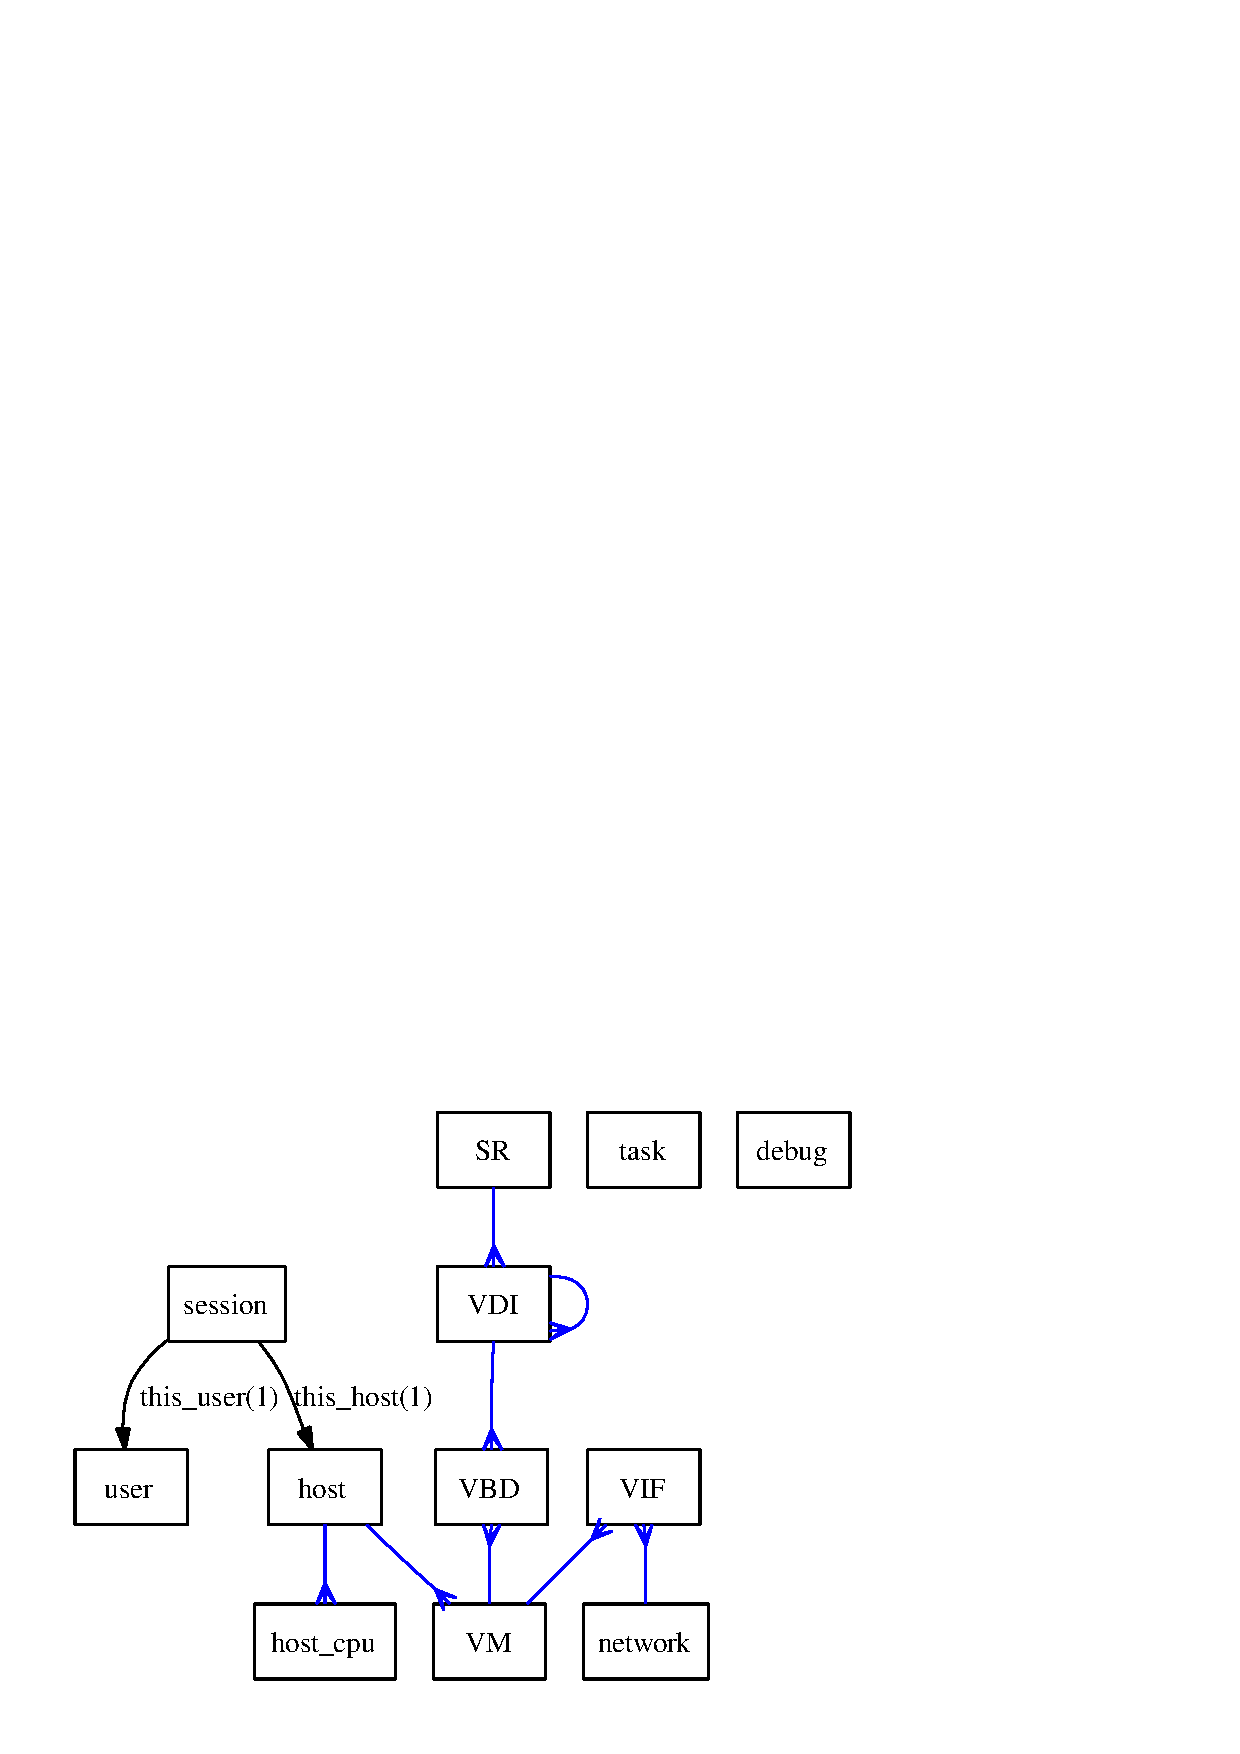
\includegraphics{xenapi-datamodel-graph}
}\end{center}
\
\subsection{List of bound fields}
\section{Types}
\subsection{Primitives}
The following primitive types are used to specify methods and fields in the API Reference:

\begin{center}\begin{tabular}{|ll|}
\hline
Type & Description \\
\hline
String & text strings \\
Int    & 64-bit integers \\
Float & IEEE double-precision floating-point numbers \\
Bool   & boolean \\
DateTime & date and timestamp \\
Ref (object name) & reference to an object of class name \\
\hline
\end{tabular}\end{center}
\subsection{Higher order types}
The following type constructors are used:

\begin{center}\begin{tabular}{|ll|}
\hline
Type & Description \\
\hline
List (t) & an arbitrary-length list of elements of type t \\
Map (a $\rightarrow$ b) & a table mapping values of type a to values of type b \\
\hline
\end{tabular}\end{center}
\subsection{Enumeration types}
The following enumeration types are used:

\begin{longtable}{|ll|}
\hline
{\tt enum console\_protocol} & \\
\hline
\hspace{0.5cm}{\tt vt100} & VT100 terminal \\
\hspace{0.5cm}{\tt rfb} & Remote FrameBuffer protocol (as used in VNC) \\
\hspace{0.5cm}{\tt rdp} & Remote Desktop Protocol \\
\hline
\end{longtable}

\vspace{1cm}
\begin{longtable}{|ll|}
\hline
{\tt enum vdi\_type} & \\
\hline
\hspace{0.5cm}{\tt system} & a disk that may be replaced on upgrade \\
\hspace{0.5cm}{\tt user} & a disk that is always preserved on upgrade \\
\hspace{0.5cm}{\tt ephemeral} & a disk that may be reformatted on upgrade \\
\hspace{0.5cm}{\tt suspend} & a disk that stores a suspend image \\
\hspace{0.5cm}{\tt crashdump} & a disk that stores VM crashdump information \\
\hline
\end{longtable}

\vspace{1cm}
\begin{longtable}{|ll|}
\hline
{\tt enum vm\_power\_state} & \\
\hline
\hspace{0.5cm}{\tt Halted} & Halted \\
\hspace{0.5cm}{\tt Paused} & Paused \\
\hspace{0.5cm}{\tt Running} & Running \\
\hspace{0.5cm}{\tt Suspended} & Suspended \\
\hspace{0.5cm}{\tt Unknown} & Some other unknown state \\
\hline
\end{longtable}

\vspace{1cm}
\begin{longtable}{|ll|}
\hline
{\tt enum task\_allowed\_operations} & \\
\hline
\hspace{0.5cm}{\tt Cancel} & Cancel \\
\hline
\end{longtable}

\vspace{1cm}
\begin{longtable}{|ll|}
\hline
{\tt enum task\_status\_type} & \\
\hline
\hspace{0.5cm}{\tt pending} & task is in progress \\
\hspace{0.5cm}{\tt success} & task was completed successfully \\
\hspace{0.5cm}{\tt failure} & task has failed \\
\hspace{0.5cm}{\tt cancelling} & task is being cancelled \\
\hspace{0.5cm}{\tt cancelled} & task has been cancelled \\
\hline
\end{longtable}

\vspace{1cm}
\begin{longtable}{|ll|}
\hline
{\tt enum on\_normal\_exit} & \\
\hline
\hspace{0.5cm}{\tt destroy} & destroy the VM state \\
\hspace{0.5cm}{\tt restart} & restart the VM \\
\hline
\end{longtable}

\vspace{1cm}
\begin{longtable}{|ll|}
\hline
{\tt enum on\_crash\_behaviour} & \\
\hline
\hspace{0.5cm}{\tt destroy} & destroy the VM state \\
\hspace{0.5cm}{\tt coredump\_and\_destroy} & record a coredump and then destroy the VM state \\
\hspace{0.5cm}{\tt restart} & restart the VM \\
\hspace{0.5cm}{\tt coredump\_and\_restart} & record a coredump and then restart the VM \\
\hspace{0.5cm}{\tt preserve} & leave the crashed VM as-is \\
\hspace{0.5cm}{\tt rename\_restart} & rename the crashed VM and start a new copy \\
\hline
\end{longtable}

\vspace{1cm}
\begin{longtable}{|ll|}
\hline
{\tt enum vbd\_mode} & \\
\hline
\hspace{0.5cm}{\tt RO} & disk is mounted read-only \\
\hspace{0.5cm}{\tt RW} & disk is mounted read-write \\
\hline
\end{longtable}

\vspace{1cm}
\begin{longtable}{|ll|}
\hline
{\tt enum vbd\_type} & \\
\hline
\hspace{0.5cm}{\tt CD} & VBD will appear to guest as CD \\
\hspace{0.5cm}{\tt Disk} & VBD will appear to guest as disk \\
\hline
\end{longtable}

\vspace{1cm}

\newpage
\section{Class: session}
\subsection{Fields for class: session}
\begin{longtable}{|lllp{0.38\textwidth}|}
\hline
\multicolumn{1}{|l}{Name} & \multicolumn{3}{l|}{\bf session} \\
\multicolumn{1}{|l}{Description} & \multicolumn{3}{l|}{\parbox{11cm}{\em A
session.}} \\
\hline
Quals & Field & Type & Description \\
\hline
$\mathit{RO}_\mathit{run}$ &  {\tt uuid} & string & unique identifier/object reference \\
$\mathit{RO}_\mathit{run}$ &  {\tt this\_host} & host ref & Currently connected host \\
$\mathit{RO}_\mathit{run}$ &  {\tt this\_user} & user ref & Currently connected user \\
$\mathit{RO}_\mathit{run}$ &  {\tt last\_active} & int & Timestamp for last time session was active \\
\hline
\end{longtable}
\subsection{Additional RPCs associated with class: session}
\subsubsection{RPC name:~login\_with\_password}

{\bf Overview:} 
Attempt to authenticate the user, returning a session\_id if successful.

 \noindent {\bf Signature:} 
\begin{verbatim} (session ref) login_with_password (string uname, string pwd)\end{verbatim}


\noindent{\bf Arguments:}

 
\vspace{0.3cm}
\begin{tabular}{|c|c|p{7cm}|}
 \hline
{\bf type} & {\bf name} & {\bf description} \\ \hline
{\tt string } & uname & Username for login. \\ \hline 

{\tt string } & pwd & Password for login. \\ \hline 

\end{tabular}

\vspace{0.3cm}

 \noindent {\bf Return Type:} 
{\tt 
session ref
}


ID of newly created session
\vspace{0.3cm}
\vspace{0.3cm}
\vspace{0.3cm}
\subsubsection{RPC name:~logout}

{\bf Overview:} 
Log out of a session.

 \noindent {\bf Signature:} 
\begin{verbatim} void logout (session_id s)\end{verbatim}


\vspace{0.3cm}

 \noindent {\bf Return Type:} 
{\tt 
void
}



\vspace{0.3cm}
\vspace{0.3cm}
\vspace{0.3cm}
\subsubsection{RPC name:~get\_uuid}

{\bf Overview:} 
Get the uuid field of the given session.

 \noindent {\bf Signature:} 
\begin{verbatim} string get_uuid (session_id s, session ref self)\end{verbatim}


\noindent{\bf Arguments:}

 
\vspace{0.3cm}
\begin{tabular}{|c|c|p{7cm}|}
 \hline
{\bf type} & {\bf name} & {\bf description} \\ \hline
{\tt session ref } & self & reference to the object \\ \hline 

\end{tabular}

\vspace{0.3cm}

 \noindent {\bf Return Type:} 
{\tt 
string
}


value of the field
\vspace{0.3cm}
\vspace{0.3cm}
\vspace{0.3cm}
\subsubsection{RPC name:~get\_this\_host}

{\bf Overview:} 
Get the this\_host field of the given session.

 \noindent {\bf Signature:} 
\begin{verbatim} (host ref) get_this_host (session_id s, session ref self)\end{verbatim}


\noindent{\bf Arguments:}

 
\vspace{0.3cm}
\begin{tabular}{|c|c|p{7cm}|}
 \hline
{\bf type} & {\bf name} & {\bf description} \\ \hline
{\tt session ref } & self & reference to the object \\ \hline 

\end{tabular}

\vspace{0.3cm}

 \noindent {\bf Return Type:} 
{\tt 
host ref
}


value of the field
\vspace{0.3cm}
\vspace{0.3cm}
\vspace{0.3cm}
\subsubsection{RPC name:~get\_this\_user}

{\bf Overview:} 
Get the this\_user field of the given session.

 \noindent {\bf Signature:} 
\begin{verbatim} (user ref) get_this_user (session_id s, session ref self)\end{verbatim}


\noindent{\bf Arguments:}

 
\vspace{0.3cm}
\begin{tabular}{|c|c|p{7cm}|}
 \hline
{\bf type} & {\bf name} & {\bf description} \\ \hline
{\tt session ref } & self & reference to the object \\ \hline 

\end{tabular}

\vspace{0.3cm}

 \noindent {\bf Return Type:} 
{\tt 
user ref
}


value of the field
\vspace{0.3cm}
\vspace{0.3cm}
\vspace{0.3cm}
\subsubsection{RPC name:~get\_last\_active}

{\bf Overview:} 
Get the last\_active field of the given session.

 \noindent {\bf Signature:} 
\begin{verbatim} int get_last_active (session_id s, session ref self)\end{verbatim}


\noindent{\bf Arguments:}

 
\vspace{0.3cm}
\begin{tabular}{|c|c|p{7cm}|}
 \hline
{\bf type} & {\bf name} & {\bf description} \\ \hline
{\tt session ref } & self & reference to the object \\ \hline 

\end{tabular}

\vspace{0.3cm}

 \noindent {\bf Return Type:} 
{\tt 
int
}


value of the field
\vspace{0.3cm}
\vspace{0.3cm}
\vspace{0.3cm}
\subsubsection{RPC name:~get\_by\_uuid}

{\bf Overview:} 
Get a reference to the session instance with the specified UUID.

 \noindent {\bf Signature:} 
\begin{verbatim} (session ref) get_by_uuid (session_id s, string uuid)\end{verbatim}


\noindent{\bf Arguments:}

 
\vspace{0.3cm}
\begin{tabular}{|c|c|p{7cm}|}
 \hline
{\bf type} & {\bf name} & {\bf description} \\ \hline
{\tt string } & uuid & UUID of object to return \\ \hline 

\end{tabular}

\vspace{0.3cm}

 \noindent {\bf Return Type:} 
{\tt 
session ref
}


reference to the object
\vspace{0.3cm}
\vspace{0.3cm}
\vspace{0.3cm}
\subsubsection{RPC name:~get\_record}

{\bf Overview:} 
Get a record containing the current state of the given session.

 \noindent {\bf Signature:} 
\begin{verbatim} (session record) get_record (session_id s, session ref self)\end{verbatim}


\noindent{\bf Arguments:}

 
\vspace{0.3cm}
\begin{tabular}{|c|c|p{7cm}|}
 \hline
{\bf type} & {\bf name} & {\bf description} \\ \hline
{\tt session ref } & self & reference to the object \\ \hline 

\end{tabular}

\vspace{0.3cm}

 \noindent {\bf Return Type:} 
{\tt 
session record
}


all fields from the object
\vspace{0.3cm}
\vspace{0.3cm}
\vspace{0.3cm}

\vspace{1cm}
\newpage
\section{Class: task}
\subsection{Fields for class: task}
\begin{longtable}{|lllp{0.38\textwidth}|}
\hline
\multicolumn{1}{|l}{Name} & \multicolumn{3}{l|}{\bf task} \\
\multicolumn{1}{|l}{Description} & \multicolumn{3}{l|}{\parbox{11cm}{\em A
long-running asynchronous task.}} \\
\hline
Quals & Field & Type & Description \\
\hline
$\mathit{RO}_\mathit{run}$ &  {\tt uuid} & string & unique identifier/object reference \\
$\mathit{RO}_\mathit{run}$ &  {\tt name/label} & string & a human-readable name \\
$\mathit{RO}_\mathit{run}$ &  {\tt name/description} & string & a notes field containg human-readable description \\
$\mathit{RO}_\mathit{run}$ &  {\tt status} & task\_status\_type & current status of the task \\
$\mathit{RO}_\mathit{run}$ &  {\tt session} & session ref & the session that created the task \\
$\mathit{RO}_\mathit{run}$ &  {\tt progress} & int & if the task is still pending, this field contains the estimated percentage complete (0-100). If task has completed (successfully or unsuccessfully) this should be 100. \\
$\mathit{RO}_\mathit{run}$ &  {\tt type} & string & if the task has completed successfully, this field contains the type of the encoded result (i.e. name of the class whose reference is in the result field). Undefined otherwise. \\
$\mathit{RO}_\mathit{run}$ &  {\tt result} & string & if the task has completed successfully, this field contains the result value (either Void or an object reference). Undefined otherwise. \\
$\mathit{RO}_\mathit{run}$ &  {\tt error\_code} & int & if the task has failed, this field contains the error code. Undefined otherwise. \\
$\mathit{RO}_\mathit{run}$ &  {\tt error\_info} & string Set & if the task has failed, this field contains the set of associated error strings. Undefined otherwise. \\
$\mathit{RO}_\mathit{run}$ &  {\tt allowed\_operations} & (task\_allowed\_operations) Set & Operations allowed on this task \\
\hline
\end{longtable}
\subsection{Additional RPCs associated with class: task}
\subsubsection{RPC name:~cancel}

{\bf Overview:} 
Cancel this task.  If task.allowed\_operations does not contain Cancel,
then this will fail with OPERATION\_NOT\_ALLOWED.  The task will show the
status 'cancelling', and you should continue to check its status until it
shows 'cancelled'.  There is no guarantee as to the time within which this
task will be cancelled.

 \noindent {\bf Signature:} 
\begin{verbatim} void cancel (session_id s, task ref task)\end{verbatim}


\noindent{\bf Arguments:}

 
\vspace{0.3cm}
\begin{tabular}{|c|c|p{7cm}|}
 \hline
{\bf type} & {\bf name} & {\bf description} \\ \hline
{\tt task ref } & task & The task \\ \hline 

\end{tabular}

\vspace{0.3cm}

 \noindent {\bf Return Type:} 
{\tt 
void
}



\vspace{0.3cm}

\noindent{\bf Possible Error Codes:} {\tt OPERATION\_NOT\_ALLOWED}

\vspace{0.6cm}
\subsubsection{RPC name:~get\_all}

{\bf Overview:} 
Return a list of all the tasks known to the system.

 \noindent {\bf Signature:} 
\begin{verbatim} ((task ref) Set) get_all (session_id s)\end{verbatim}


\vspace{0.3cm}

 \noindent {\bf Return Type:} 
{\tt 
(task ref) Set
}


references to all objects
\vspace{0.3cm}
\vspace{0.3cm}
\vspace{0.3cm}
\subsubsection{RPC name:~get\_uuid}

{\bf Overview:} 
Get the uuid field of the given task.

 \noindent {\bf Signature:} 
\begin{verbatim} string get_uuid (session_id s, task ref self)\end{verbatim}


\noindent{\bf Arguments:}

 
\vspace{0.3cm}
\begin{tabular}{|c|c|p{7cm}|}
 \hline
{\bf type} & {\bf name} & {\bf description} \\ \hline
{\tt task ref } & self & reference to the object \\ \hline 

\end{tabular}

\vspace{0.3cm}

 \noindent {\bf Return Type:} 
{\tt 
string
}


value of the field
\vspace{0.3cm}
\vspace{0.3cm}
\vspace{0.3cm}
\subsubsection{RPC name:~get\_name\_label}

{\bf Overview:} 
Get the name/label field of the given task.

 \noindent {\bf Signature:} 
\begin{verbatim} string get_name_label (session_id s, task ref self)\end{verbatim}


\noindent{\bf Arguments:}

 
\vspace{0.3cm}
\begin{tabular}{|c|c|p{7cm}|}
 \hline
{\bf type} & {\bf name} & {\bf description} \\ \hline
{\tt task ref } & self & reference to the object \\ \hline 

\end{tabular}

\vspace{0.3cm}

 \noindent {\bf Return Type:} 
{\tt 
string
}


value of the field
\vspace{0.3cm}
\vspace{0.3cm}
\vspace{0.3cm}
\subsubsection{RPC name:~get\_name\_description}

{\bf Overview:} 
Get the name/description field of the given task.

 \noindent {\bf Signature:} 
\begin{verbatim} string get_name_description (session_id s, task ref self)\end{verbatim}


\noindent{\bf Arguments:}

 
\vspace{0.3cm}
\begin{tabular}{|c|c|p{7cm}|}
 \hline
{\bf type} & {\bf name} & {\bf description} \\ \hline
{\tt task ref } & self & reference to the object \\ \hline 

\end{tabular}

\vspace{0.3cm}

 \noindent {\bf Return Type:} 
{\tt 
string
}


value of the field
\vspace{0.3cm}
\vspace{0.3cm}
\vspace{0.3cm}
\subsubsection{RPC name:~get\_status}

{\bf Overview:} 
Get the status field of the given task.

 \noindent {\bf Signature:} 
\begin{verbatim} (task_status_type) get_status (session_id s, task ref self)\end{verbatim}


\noindent{\bf Arguments:}

 
\vspace{0.3cm}
\begin{tabular}{|c|c|p{7cm}|}
 \hline
{\bf type} & {\bf name} & {\bf description} \\ \hline
{\tt task ref } & self & reference to the object \\ \hline 

\end{tabular}

\vspace{0.3cm}

 \noindent {\bf Return Type:} 
{\tt 
task\_status\_type
}


value of the field
\vspace{0.3cm}
\vspace{0.3cm}
\vspace{0.3cm}
\subsubsection{RPC name:~get\_session}

{\bf Overview:} 
Get the session field of the given task.

 \noindent {\bf Signature:} 
\begin{verbatim} (session ref) get_session (session_id s, task ref self)\end{verbatim}


\noindent{\bf Arguments:}

 
\vspace{0.3cm}
\begin{tabular}{|c|c|p{7cm}|}
 \hline
{\bf type} & {\bf name} & {\bf description} \\ \hline
{\tt task ref } & self & reference to the object \\ \hline 

\end{tabular}

\vspace{0.3cm}

 \noindent {\bf Return Type:} 
{\tt 
session ref
}


value of the field
\vspace{0.3cm}
\vspace{0.3cm}
\vspace{0.3cm}
\subsubsection{RPC name:~get\_progress}

{\bf Overview:} 
Get the progress field of the given task.

 \noindent {\bf Signature:} 
\begin{verbatim} int get_progress (session_id s, task ref self)\end{verbatim}


\noindent{\bf Arguments:}

 
\vspace{0.3cm}
\begin{tabular}{|c|c|p{7cm}|}
 \hline
{\bf type} & {\bf name} & {\bf description} \\ \hline
{\tt task ref } & self & reference to the object \\ \hline 

\end{tabular}

\vspace{0.3cm}

 \noindent {\bf Return Type:} 
{\tt 
int
}


value of the field
\vspace{0.3cm}
\vspace{0.3cm}
\vspace{0.3cm}
\subsubsection{RPC name:~get\_type}

{\bf Overview:} 
Get the type field of the given task.

 \noindent {\bf Signature:} 
\begin{verbatim} string get_type (session_id s, task ref self)\end{verbatim}


\noindent{\bf Arguments:}

 
\vspace{0.3cm}
\begin{tabular}{|c|c|p{7cm}|}
 \hline
{\bf type} & {\bf name} & {\bf description} \\ \hline
{\tt task ref } & self & reference to the object \\ \hline 

\end{tabular}

\vspace{0.3cm}

 \noindent {\bf Return Type:} 
{\tt 
string
}


value of the field
\vspace{0.3cm}
\vspace{0.3cm}
\vspace{0.3cm}
\subsubsection{RPC name:~get\_result}

{\bf Overview:} 
Get the result field of the given task.

 \noindent {\bf Signature:} 
\begin{verbatim} string get_result (session_id s, task ref self)\end{verbatim}


\noindent{\bf Arguments:}

 
\vspace{0.3cm}
\begin{tabular}{|c|c|p{7cm}|}
 \hline
{\bf type} & {\bf name} & {\bf description} \\ \hline
{\tt task ref } & self & reference to the object \\ \hline 

\end{tabular}

\vspace{0.3cm}

 \noindent {\bf Return Type:} 
{\tt 
string
}


value of the field
\vspace{0.3cm}
\vspace{0.3cm}
\vspace{0.3cm}
\subsubsection{RPC name:~get\_error\_code}

{\bf Overview:} 
Get the error\_code field of the given task.

 \noindent {\bf Signature:} 
\begin{verbatim} int get_error_code (session_id s, task ref self)\end{verbatim}


\noindent{\bf Arguments:}

 
\vspace{0.3cm}
\begin{tabular}{|c|c|p{7cm}|}
 \hline
{\bf type} & {\bf name} & {\bf description} \\ \hline
{\tt task ref } & self & reference to the object \\ \hline 

\end{tabular}

\vspace{0.3cm}

 \noindent {\bf Return Type:} 
{\tt 
int
}


value of the field
\vspace{0.3cm}
\vspace{0.3cm}
\vspace{0.3cm}
\subsubsection{RPC name:~get\_error\_info}

{\bf Overview:} 
Get the error\_info field of the given task.

 \noindent {\bf Signature:} 
\begin{verbatim} (string Set) get_error_info (session_id s, task ref self)\end{verbatim}


\noindent{\bf Arguments:}

 
\vspace{0.3cm}
\begin{tabular}{|c|c|p{7cm}|}
 \hline
{\bf type} & {\bf name} & {\bf description} \\ \hline
{\tt task ref } & self & reference to the object \\ \hline 

\end{tabular}

\vspace{0.3cm}

 \noindent {\bf Return Type:} 
{\tt 
string Set
}


value of the field
\vspace{0.3cm}
\vspace{0.3cm}
\vspace{0.3cm}
\subsubsection{RPC name:~get\_allowed\_operations}

{\bf Overview:} 
Get the allowed\_operations field of the given task.

 \noindent {\bf Signature:} 
\begin{verbatim} ((task_allowed_operations) Set) get_allowed_operations (session_id s, task ref self)\end{verbatim}


\noindent{\bf Arguments:}

 
\vspace{0.3cm}
\begin{tabular}{|c|c|p{7cm}|}
 \hline
{\bf type} & {\bf name} & {\bf description} \\ \hline
{\tt task ref } & self & reference to the object \\ \hline 

\end{tabular}

\vspace{0.3cm}

 \noindent {\bf Return Type:} 
{\tt 
(task\_allowed\_operations) Set
}


value of the field
\vspace{0.3cm}
\vspace{0.3cm}
\vspace{0.3cm}
\subsubsection{RPC name:~get\_by\_uuid}

{\bf Overview:} 
Get a reference to the task instance with the specified UUID.

 \noindent {\bf Signature:} 
\begin{verbatim} (task ref) get_by_uuid (session_id s, string uuid)\end{verbatim}


\noindent{\bf Arguments:}

 
\vspace{0.3cm}
\begin{tabular}{|c|c|p{7cm}|}
 \hline
{\bf type} & {\bf name} & {\bf description} \\ \hline
{\tt string } & uuid & UUID of object to return \\ \hline 

\end{tabular}

\vspace{0.3cm}

 \noindent {\bf Return Type:} 
{\tt 
task ref
}


reference to the object
\vspace{0.3cm}
\vspace{0.3cm}
\vspace{0.3cm}
\subsubsection{RPC name:~get\_record}

{\bf Overview:} 
Get a record containing the current state of the given task.

 \noindent {\bf Signature:} 
\begin{verbatim} (task record) get_record (session_id s, task ref self)\end{verbatim}


\noindent{\bf Arguments:}

 
\vspace{0.3cm}
\begin{tabular}{|c|c|p{7cm}|}
 \hline
{\bf type} & {\bf name} & {\bf description} \\ \hline
{\tt task ref } & self & reference to the object \\ \hline 

\end{tabular}

\vspace{0.3cm}

 \noindent {\bf Return Type:} 
{\tt 
task record
}


all fields from the object
\vspace{0.3cm}
\vspace{0.3cm}
\vspace{0.3cm}
\subsubsection{RPC name:~get\_by\_name\_label}

{\bf Overview:} 
Get all the task instances with the given label.

 \noindent {\bf Signature:} 
\begin{verbatim} ((task ref) Set) get_by_name_label (session_id s, string label)\end{verbatim}


\noindent{\bf Arguments:}

 
\vspace{0.3cm}
\begin{tabular}{|c|c|p{7cm}|}
 \hline
{\bf type} & {\bf name} & {\bf description} \\ \hline
{\tt string } & label & label of object to return \\ \hline 

\end{tabular}

\vspace{0.3cm}

 \noindent {\bf Return Type:} 
{\tt 
(task ref) Set
}


references to objects with match names
\vspace{0.3cm}
\vspace{0.3cm}
\vspace{0.3cm}

\vspace{1cm}
\newpage
\section{Class: VM}
\subsection{Fields for class: VM}
\begin{longtable}{|lllp{0.38\textwidth}|}
\hline
\multicolumn{1}{|l}{Name} & \multicolumn{3}{l|}{\bf VM} \\
\multicolumn{1}{|l}{Description} & \multicolumn{3}{l|}{\parbox{11cm}{\em A
virtual machine (or 'guest').

VM booting is controlled by setting one of the two mutually exclusive
groups: "PV", and "HVM".  If HVM.boot\_policy is the empty string, then
paravirtual domain building and booting will be used; otherwise the VM will
be loaded as an HVM domain, and booted using an emulated BIOS.

When paravirtual booting is in use, the PV/bootloader field indicates the
bootloader to use.  It may be "pygrub", in which case the platform's
default installation of pygrub will be used, or a full path within the
control domain to some other bootloader.  The other fields, PV/kernel,
PV/ramdisk, PV/args and PV/bootloader\_args will be passed to the
bootloader unmodified, and interpretation of those fields is then specific
to the bootloader itself, including the possibility that the bootloader
will ignore some or all of those given values. Finally the paths of all
bootable disks are added to the bootloader commandline (a disk is bootable
if its VBD has the bootable flag set). There may be zero, one or many
bootable disks; the bootloader decides which disk (if any) to boot from.

If the bootloader is pygrub, then the menu.lst is parsed if present in the
guest's filesystem, otherwise the specified kernel and ramdisk are used, or
an autodetected kernel is used if nothing is specified and autodetection is
possible.  PV/args is appended to the kernel command line, no matter which
mechanism is used for finding the kernel.

If PV/bootloader is empty but PV/kernel is specified, then the kernel and
ramdisk values will be treated as paths within the control domain.  If both
PV/bootloader and PV/kernel are empty, then the behaviour is as if
PV/bootloader was specified as "pygrub".

When using HVM booting, HVM/boot\_policy and HVM/boot\_params specify the
boot handling.  Only one policy is currently defined: "BIOS order".  In
this case, HVM/boot\_params should contain one key-value pair "order" = "N"
where N is the string that will be passed to QEMU.}} \\
\hline
Quals & Field & Type & Description \\
\hline
$\mathit{RO}_\mathit{run}$ &  {\tt uuid} & string & unique identifier/object reference \\
$\mathit{RO}_\mathit{run}$ &  {\tt power\_state} & vm\_power\_state & Current power state of the machine \\
$\mathit{RW}$ &  {\tt name/label} & string & a human-readable name \\
$\mathit{RW}$ &  {\tt name/description} & string & a notes field containg human-readable description \\
$\mathit{RW}$ &  {\tt user\_version} & int & a user version number for this machine \\
$\mathit{RW}$ &  {\tt is\_a\_template} & bool & true if this is a template. Template VMs can never be started, they are used only for cloning other VMs \\
$\mathit{RW}$ &  {\tt auto\_power\_on} & bool & true if this VM should be started automatically after host boot \\
$\mathit{RO}_\mathit{run}$ &  {\tt suspend\_VDI} & VDI ref & The VDI that a suspend image is stored on. (Only has meaning if VM is currently suspended) \\
$\mathit{RO}_\mathit{run}$ &  {\tt resident\_on} & host ref & the host the VM is currently resident on \\
$\mathit{RW}$ &  {\tt memory/static\_max} & int & Statically-set (i.e. absolute) maximum (bytes) \\
$\mathit{RW}$ &  {\tt memory/dynamic\_max} & int & Dynamic maximum (bytes) \\
$\mathit{RW}$ &  {\tt memory/dynamic\_min} & int & Dynamic minimum (bytes) \\
$\mathit{RW}$ &  {\tt memory/static\_min} & int & Statically-set (i.e. absolute) mininum (bytes) \\
$\mathit{RW}$ &  {\tt VCPUs/policy} & string & the name of the VCPU scheduling policy to be applied \\
$\mathit{RW}$ &  {\tt VCPUs/params} & (string $\rightarrow$ string) Map & configuration parameters for the selected VCPU policy \\
$\mathit{RW}$ &  {\tt VCPUs/max} & int & Max number of VCPUs \\
$\mathit{RW}$ &  {\tt VCPUs/at\_startup} & int & Boot number of VCPUs \\
$\mathit{RW}$ &  {\tt actions/after\_shutdown} & on\_normal\_exit & action to take after the guest has shutdown itself \\
$\mathit{RW}$ &  {\tt actions/after\_reboot} & on\_normal\_exit & action to take after the guest has rebooted itself \\
$\mathit{RW}$ &  {\tt actions/after\_crash} & on\_crash\_behaviour & action to take if the guest crashes \\
$\mathit{RO}_\mathit{run}$ &  {\tt consoles} & (console ref) Set & virtual console devices \\
$\mathit{RO}_\mathit{run}$ &  {\tt VIFs} & (VIF ref) Set & virtual network interfaces \\
$\mathit{RO}_\mathit{run}$ &  {\tt VBDs} & (VBD ref) Set & virtual block devices \\
$\mathit{RO}_\mathit{run}$ &  {\tt crash\_dumps} & (crashdump ref) Set & crash dumps associated with this VM \\
$\mathit{RO}_\mathit{run}$ &  {\tt VTPMs} & (VTPM ref) Set & virtual TPMs \\
$\mathit{RW}$ &  {\tt PV/bootloader} & string & name of or path to bootloader \\
$\mathit{RW}$ &  {\tt PV/kernel} & string & path to the kernel \\
$\mathit{RW}$ &  {\tt PV/ramdisk} & string & path to the initrd \\
$\mathit{RW}$ &  {\tt PV/args} & string & kernel command-line arguments \\
$\mathit{RW}$ &  {\tt PV/bootloader\_args} & string & miscellaneous arguments for the bootloader \\
$\mathit{RW}$ &  {\tt HVM/boot\_policy} & string & HVM boot policy \\
$\mathit{RW}$ &  {\tt HVM/boot\_params} & (string $\rightarrow$ string) Map & HVM boot params \\
$\mathit{RW}$ &  {\tt platform/std\_VGA} & bool & emulate standard VGA instead of cirrus logic \\
$\mathit{RW}$ &  {\tt platform/serial} & string & redirect serial port to pty \\
$\mathit{RW}$ &  {\tt platform/localtime} & bool & set RTC to local time \\
$\mathit{RW}$ &  {\tt platform/clock\_offset} & bool & timeshift applied to guest's clock \\
$\mathit{RW}$ &  {\tt platform/enable\_audio} & bool & emulate audio \\
$\mathit{RO}_\mathit{ins}$ &  {\tt PCI\_bus} & string & PCI bus path for pass-through devices \\
$\mathit{RW}$ &  {\tt other\_config} & (string $\rightarrow$ string) Map & additional configuration \\
$\mathit{RO}_\mathit{run}$ &  {\tt domid} & int & domain ID (if available, -1 otherwise) \\
$\mathit{RO}_\mathit{run}$ &  {\tt is\_control\_domain} & bool & true if this is a control domain (domain 0 or a driver domain) \\
$\mathit{RO}_\mathit{run}$ &  {\tt metrics} & VM\_metrics ref & metrics associated with this VM. \\
$\mathit{RO}_\mathit{run}$ &  {\tt guest\_metrics} & VM\_guest\_metrics ref & metrics associated with the running guest \\
\hline
\end{longtable}
\subsection{Additional RPCs associated with class: VM}
\subsubsection{RPC name:~clone}

{\bf Overview:} 
Clones the specified VM, making a new VM. Clone automatically exploits the
capabilities of the underlying storage repository in which the VM's disk
images are stored (e.g. Copy on Write).   This function can only be called
when the VM is in the Halted State.

 \noindent {\bf Signature:} 
\begin{verbatim} (VM ref) clone (session_id s, VM ref vm, string new_name)\end{verbatim}


\noindent{\bf Arguments:}

 
\vspace{0.3cm}
\begin{tabular}{|c|c|p{7cm}|}
 \hline
{\bf type} & {\bf name} & {\bf description} \\ \hline
{\tt VM ref } & vm & The VM to be cloned \\ \hline 

{\tt string } & new\_name & The name of the cloned VM \\ \hline 

\end{tabular}

\vspace{0.3cm}

 \noindent {\bf Return Type:} 
{\tt 
VM ref
}


The ID of the newly created VM.
\vspace{0.3cm}

\noindent{\bf Possible Error Codes:} {\tt VM\_BAD\_POWER\_STATE}

\vspace{0.6cm}
\subsubsection{RPC name:~start}

{\bf Overview:} 
Start the specified VM.  This function can only be called with the VM is in
the Halted State.

 \noindent {\bf Signature:} 
\begin{verbatim} void start (session_id s, VM ref vm, bool start_paused)\end{verbatim}


\noindent{\bf Arguments:}

 
\vspace{0.3cm}
\begin{tabular}{|c|c|p{7cm}|}
 \hline
{\bf type} & {\bf name} & {\bf description} \\ \hline
{\tt VM ref } & vm & The VM to start \\ \hline 

{\tt bool } & start\_paused & Instantiate VM in paused state if set to true. \\ \hline 

\end{tabular}

\vspace{0.3cm}

 \noindent {\bf Return Type:} 
{\tt 
void
}



\vspace{0.3cm}

\noindent{\bf Possible Error Codes:} {\tt VM\_BAD\_POWER\_STATE}

\vspace{0.6cm}
\subsubsection{RPC name:~pause}

{\bf Overview:} 
Pause the specified VM. This can only be called when the specified VM is in
the Running state.

 \noindent {\bf Signature:} 
\begin{verbatim} void pause (session_id s, VM ref vm)\end{verbatim}


\noindent{\bf Arguments:}

 
\vspace{0.3cm}
\begin{tabular}{|c|c|p{7cm}|}
 \hline
{\bf type} & {\bf name} & {\bf description} \\ \hline
{\tt VM ref } & vm & The VM to pause \\ \hline 

\end{tabular}

\vspace{0.3cm}

 \noindent {\bf Return Type:} 
{\tt 
void
}



\vspace{0.3cm}

\noindent{\bf Possible Error Codes:} {\tt VM\_BAD\_POWER\_STATE}

\vspace{0.6cm}
\subsubsection{RPC name:~unpause}

{\bf Overview:} 
Resume the specified VM. This can only be called when the specified VM is
in the Paused state.

 \noindent {\bf Signature:} 
\begin{verbatim} void unpause (session_id s, VM ref vm)\end{verbatim}


\noindent{\bf Arguments:}

 
\vspace{0.3cm}
\begin{tabular}{|c|c|p{7cm}|}
 \hline
{\bf type} & {\bf name} & {\bf description} \\ \hline
{\tt VM ref } & vm & The VM to unpause \\ \hline 

\end{tabular}

\vspace{0.3cm}

 \noindent {\bf Return Type:} 
{\tt 
void
}



\vspace{0.3cm}

\noindent{\bf Possible Error Codes:} {\tt VM\_BAD\_POWER\_STATE}

\vspace{0.6cm}
\subsubsection{RPC name:~clean\_shutdown}

{\bf Overview:} 
Attempt to cleanly shutdown the specified VM. (Note: this may not be
supported---e.g. if a guest agent is not installed).

Once shutdown has been completed perform poweroff action specified in guest
configuration.

This can only be called when the specified VM is in the Running state.

 \noindent {\bf Signature:} 
\begin{verbatim} void clean_shutdown (session_id s, VM ref vm)\end{verbatim}


\noindent{\bf Arguments:}

 
\vspace{0.3cm}
\begin{tabular}{|c|c|p{7cm}|}
 \hline
{\bf type} & {\bf name} & {\bf description} \\ \hline
{\tt VM ref } & vm & The VM to shutdown \\ \hline 

\end{tabular}

\vspace{0.3cm}

 \noindent {\bf Return Type:} 
{\tt 
void
}



\vspace{0.3cm}

\noindent{\bf Possible Error Codes:} {\tt VM\_BAD\_POWER\_STATE}

\vspace{0.6cm}
\subsubsection{RPC name:~clean\_reboot}

{\bf Overview:} 
Attempt to cleanly shutdown the specified VM (Note: this may not be
supported---e.g. if a guest agent is not installed).

Once shutdown has been completed perform reboot action specified in guest
configuration.

This can only be called when the specified VM is in the Running state.

 \noindent {\bf Signature:} 
\begin{verbatim} void clean_reboot (session_id s, VM ref vm)\end{verbatim}


\noindent{\bf Arguments:}

 
\vspace{0.3cm}
\begin{tabular}{|c|c|p{7cm}|}
 \hline
{\bf type} & {\bf name} & {\bf description} \\ \hline
{\tt VM ref } & vm & The VM to shutdown \\ \hline 

\end{tabular}

\vspace{0.3cm}

 \noindent {\bf Return Type:} 
{\tt 
void
}



\vspace{0.3cm}

\noindent{\bf Possible Error Codes:} {\tt VM\_BAD\_POWER\_STATE}

\vspace{0.6cm}
\subsubsection{RPC name:~hard\_shutdown}

{\bf Overview:} 
Stop executing the specified VM without attempting a clean shutdown. Then
perform poweroff action specified in VM configuration.

 \noindent {\bf Signature:} 
\begin{verbatim} void hard_shutdown (session_id s, VM ref vm)\end{verbatim}


\noindent{\bf Arguments:}

 
\vspace{0.3cm}
\begin{tabular}{|c|c|p{7cm}|}
 \hline
{\bf type} & {\bf name} & {\bf description} \\ \hline
{\tt VM ref } & vm & The VM to destroy \\ \hline 

\end{tabular}

\vspace{0.3cm}

 \noindent {\bf Return Type:} 
{\tt 
void
}



\vspace{0.3cm}
\vspace{0.3cm}
\vspace{0.3cm}
\subsubsection{RPC name:~hard\_reboot}

{\bf Overview:} 
Stop executing the specified VM without attempting a clean shutdown. Then
perform reboot action specified in VM configuration.

 \noindent {\bf Signature:} 
\begin{verbatim} void hard_reboot (session_id s, VM ref vm)\end{verbatim}


\noindent{\bf Arguments:}

 
\vspace{0.3cm}
\begin{tabular}{|c|c|p{7cm}|}
 \hline
{\bf type} & {\bf name} & {\bf description} \\ \hline
{\tt VM ref } & vm & The VM to reboot \\ \hline 

\end{tabular}

\vspace{0.3cm}

 \noindent {\bf Return Type:} 
{\tt 
void
}



\vspace{0.3cm}
\vspace{0.3cm}
\vspace{0.3cm}
\subsubsection{RPC name:~suspend}

{\bf Overview:} 
Suspend the specified VM to disk.  This can only be called when the
specified VM is in the Running state.

 \noindent {\bf Signature:} 
\begin{verbatim} void suspend (session_id s, VM ref vm)\end{verbatim}


\noindent{\bf Arguments:}

 
\vspace{0.3cm}
\begin{tabular}{|c|c|p{7cm}|}
 \hline
{\bf type} & {\bf name} & {\bf description} \\ \hline
{\tt VM ref } & vm & The VM to hibernate \\ \hline 

\end{tabular}

\vspace{0.3cm}

 \noindent {\bf Return Type:} 
{\tt 
void
}



\vspace{0.3cm}

\noindent{\bf Possible Error Codes:} {\tt VM\_BAD\_POWER\_STATE}

\vspace{0.6cm}
\subsubsection{RPC name:~resume}

{\bf Overview:} 
Awaken the specified VM and resume it.  This can only be called when the
specified VM is in the Suspended state.

 \noindent {\bf Signature:} 
\begin{verbatim} void resume (session_id s, VM ref vm, bool start_paused)\end{verbatim}


\noindent{\bf Arguments:}

 
\vspace{0.3cm}
\begin{tabular}{|c|c|p{7cm}|}
 \hline
{\bf type} & {\bf name} & {\bf description} \\ \hline
{\tt VM ref } & vm & The VM to unhibernate \\ \hline 

{\tt bool } & start\_paused & Unhibernate VM in paused state if set to true. \\ \hline 

\end{tabular}

\vspace{0.3cm}

 \noindent {\bf Return Type:} 
{\tt 
void
}



\vspace{0.3cm}

\noindent{\bf Possible Error Codes:} {\tt VM\_BAD\_POWER\_STATE}

\vspace{0.6cm}
\subsubsection{RPC name:~get\_all}

{\bf Overview:} 
Return a list of all the VMs known to the system.

 \noindent {\bf Signature:} 
\begin{verbatim} ((VM ref) Set) get_all (session_id s)\end{verbatim}


\vspace{0.3cm}

 \noindent {\bf Return Type:} 
{\tt 
(VM ref) Set
}


A list of all the IDs of all the VMs
\vspace{0.3cm}
\vspace{0.3cm}
\vspace{0.3cm}
\subsubsection{RPC name:~get\_uuid}

{\bf Overview:} 
Get the uuid field of the given VM.

 \noindent {\bf Signature:} 
\begin{verbatim} string get_uuid (session_id s, VM ref self)\end{verbatim}


\noindent{\bf Arguments:}

 
\vspace{0.3cm}
\begin{tabular}{|c|c|p{7cm}|}
 \hline
{\bf type} & {\bf name} & {\bf description} \\ \hline
{\tt VM ref } & self & reference to the object \\ \hline 

\end{tabular}

\vspace{0.3cm}

 \noindent {\bf Return Type:} 
{\tt 
string
}


value of the field
\vspace{0.3cm}
\vspace{0.3cm}
\vspace{0.3cm}
\subsubsection{RPC name:~get\_power\_state}

{\bf Overview:} 
Get the power\_state field of the given VM.

 \noindent {\bf Signature:} 
\begin{verbatim} (vm_power_state) get_power_state (session_id s, VM ref self)\end{verbatim}


\noindent{\bf Arguments:}

 
\vspace{0.3cm}
\begin{tabular}{|c|c|p{7cm}|}
 \hline
{\bf type} & {\bf name} & {\bf description} \\ \hline
{\tt VM ref } & self & reference to the object \\ \hline 

\end{tabular}

\vspace{0.3cm}

 \noindent {\bf Return Type:} 
{\tt 
vm\_power\_state
}


value of the field
\vspace{0.3cm}
\vspace{0.3cm}
\vspace{0.3cm}
\subsubsection{RPC name:~get\_name\_label}

{\bf Overview:} 
Get the name/label field of the given VM.

 \noindent {\bf Signature:} 
\begin{verbatim} string get_name_label (session_id s, VM ref self)\end{verbatim}


\noindent{\bf Arguments:}

 
\vspace{0.3cm}
\begin{tabular}{|c|c|p{7cm}|}
 \hline
{\bf type} & {\bf name} & {\bf description} \\ \hline
{\tt VM ref } & self & reference to the object \\ \hline 

\end{tabular}

\vspace{0.3cm}

 \noindent {\bf Return Type:} 
{\tt 
string
}


value of the field
\vspace{0.3cm}
\vspace{0.3cm}
\vspace{0.3cm}
\subsubsection{RPC name:~set\_name\_label}

{\bf Overview:} 
Set the name/label field of the given VM.

 \noindent {\bf Signature:} 
\begin{verbatim} void set_name_label (session_id s, VM ref self, string value)\end{verbatim}


\noindent{\bf Arguments:}

 
\vspace{0.3cm}
\begin{tabular}{|c|c|p{7cm}|}
 \hline
{\bf type} & {\bf name} & {\bf description} \\ \hline
{\tt VM ref } & self & reference to the object \\ \hline 

{\tt string } & value & New value to set \\ \hline 

\end{tabular}

\vspace{0.3cm}

 \noindent {\bf Return Type:} 
{\tt 
void
}



\vspace{0.3cm}
\vspace{0.3cm}
\vspace{0.3cm}
\subsubsection{RPC name:~get\_name\_description}

{\bf Overview:} 
Get the name/description field of the given VM.

 \noindent {\bf Signature:} 
\begin{verbatim} string get_name_description (session_id s, VM ref self)\end{verbatim}


\noindent{\bf Arguments:}

 
\vspace{0.3cm}
\begin{tabular}{|c|c|p{7cm}|}
 \hline
{\bf type} & {\bf name} & {\bf description} \\ \hline
{\tt VM ref } & self & reference to the object \\ \hline 

\end{tabular}

\vspace{0.3cm}

 \noindent {\bf Return Type:} 
{\tt 
string
}


value of the field
\vspace{0.3cm}
\vspace{0.3cm}
\vspace{0.3cm}
\subsubsection{RPC name:~set\_name\_description}

{\bf Overview:} 
Set the name/description field of the given VM.

 \noindent {\bf Signature:} 
\begin{verbatim} void set_name_description (session_id s, VM ref self, string value)\end{verbatim}


\noindent{\bf Arguments:}

 
\vspace{0.3cm}
\begin{tabular}{|c|c|p{7cm}|}
 \hline
{\bf type} & {\bf name} & {\bf description} \\ \hline
{\tt VM ref } & self & reference to the object \\ \hline 

{\tt string } & value & New value to set \\ \hline 

\end{tabular}

\vspace{0.3cm}

 \noindent {\bf Return Type:} 
{\tt 
void
}



\vspace{0.3cm}
\vspace{0.3cm}
\vspace{0.3cm}
\subsubsection{RPC name:~get\_user\_version}

{\bf Overview:} 
Get the user\_version field of the given VM.

 \noindent {\bf Signature:} 
\begin{verbatim} int get_user_version (session_id s, VM ref self)\end{verbatim}


\noindent{\bf Arguments:}

 
\vspace{0.3cm}
\begin{tabular}{|c|c|p{7cm}|}
 \hline
{\bf type} & {\bf name} & {\bf description} \\ \hline
{\tt VM ref } & self & reference to the object \\ \hline 

\end{tabular}

\vspace{0.3cm}

 \noindent {\bf Return Type:} 
{\tt 
int
}


value of the field
\vspace{0.3cm}
\vspace{0.3cm}
\vspace{0.3cm}
\subsubsection{RPC name:~set\_user\_version}

{\bf Overview:} 
Set the user\_version field of the given VM.

 \noindent {\bf Signature:} 
\begin{verbatim} void set_user_version (session_id s, VM ref self, int value)\end{verbatim}


\noindent{\bf Arguments:}

 
\vspace{0.3cm}
\begin{tabular}{|c|c|p{7cm}|}
 \hline
{\bf type} & {\bf name} & {\bf description} \\ \hline
{\tt VM ref } & self & reference to the object \\ \hline 

{\tt int } & value & New value to set \\ \hline 

\end{tabular}

\vspace{0.3cm}

 \noindent {\bf Return Type:} 
{\tt 
void
}



\vspace{0.3cm}
\vspace{0.3cm}
\vspace{0.3cm}
\subsubsection{RPC name:~get\_is\_a\_template}

{\bf Overview:} 
Get the is\_a\_template field of the given VM.

 \noindent {\bf Signature:} 
\begin{verbatim} bool get_is_a_template (session_id s, VM ref self)\end{verbatim}


\noindent{\bf Arguments:}

 
\vspace{0.3cm}
\begin{tabular}{|c|c|p{7cm}|}
 \hline
{\bf type} & {\bf name} & {\bf description} \\ \hline
{\tt VM ref } & self & reference to the object \\ \hline 

\end{tabular}

\vspace{0.3cm}

 \noindent {\bf Return Type:} 
{\tt 
bool
}


value of the field
\vspace{0.3cm}
\vspace{0.3cm}
\vspace{0.3cm}
\subsubsection{RPC name:~set\_is\_a\_template}

{\bf Overview:} 
Set the is\_a\_template field of the given VM.

 \noindent {\bf Signature:} 
\begin{verbatim} void set_is_a_template (session_id s, VM ref self, bool value)\end{verbatim}


\noindent{\bf Arguments:}

 
\vspace{0.3cm}
\begin{tabular}{|c|c|p{7cm}|}
 \hline
{\bf type} & {\bf name} & {\bf description} \\ \hline
{\tt VM ref } & self & reference to the object \\ \hline 

{\tt bool } & value & New value to set \\ \hline 

\end{tabular}

\vspace{0.3cm}

 \noindent {\bf Return Type:} 
{\tt 
void
}



\vspace{0.3cm}
\vspace{0.3cm}
\vspace{0.3cm}
\subsubsection{RPC name:~get\_auto\_power\_on}

{\bf Overview:} 
Get the auto\_power\_on field of the given VM.

 \noindent {\bf Signature:} 
\begin{verbatim} bool get_auto_power_on (session_id s, VM ref self)\end{verbatim}


\noindent{\bf Arguments:}

 
\vspace{0.3cm}
\begin{tabular}{|c|c|p{7cm}|}
 \hline
{\bf type} & {\bf name} & {\bf description} \\ \hline
{\tt VM ref } & self & reference to the object \\ \hline 

\end{tabular}

\vspace{0.3cm}

 \noindent {\bf Return Type:} 
{\tt 
bool
}


value of the field
\vspace{0.3cm}
\vspace{0.3cm}
\vspace{0.3cm}
\subsubsection{RPC name:~set\_auto\_power\_on}

{\bf Overview:} 
Set the auto\_power\_on field of the given VM.

 \noindent {\bf Signature:} 
\begin{verbatim} void set_auto_power_on (session_id s, VM ref self, bool value)\end{verbatim}


\noindent{\bf Arguments:}

 
\vspace{0.3cm}
\begin{tabular}{|c|c|p{7cm}|}
 \hline
{\bf type} & {\bf name} & {\bf description} \\ \hline
{\tt VM ref } & self & reference to the object \\ \hline 

{\tt bool } & value & New value to set \\ \hline 

\end{tabular}

\vspace{0.3cm}

 \noindent {\bf Return Type:} 
{\tt 
void
}



\vspace{0.3cm}
\vspace{0.3cm}
\vspace{0.3cm}
\subsubsection{RPC name:~get\_suspend\_VDI}

{\bf Overview:} 
Get the suspend\_VDI field of the given VM.

 \noindent {\bf Signature:} 
\begin{verbatim} (VDI ref) get_suspend_VDI (session_id s, VM ref self)\end{verbatim}


\noindent{\bf Arguments:}

 
\vspace{0.3cm}
\begin{tabular}{|c|c|p{7cm}|}
 \hline
{\bf type} & {\bf name} & {\bf description} \\ \hline
{\tt VM ref } & self & reference to the object \\ \hline 

\end{tabular}

\vspace{0.3cm}

 \noindent {\bf Return Type:} 
{\tt 
VDI ref
}


value of the field
\vspace{0.3cm}
\vspace{0.3cm}
\vspace{0.3cm}
\subsubsection{RPC name:~get\_resident\_on}

{\bf Overview:} 
Get the resident\_on field of the given VM.

 \noindent {\bf Signature:} 
\begin{verbatim} (host ref) get_resident_on (session_id s, VM ref self)\end{verbatim}


\noindent{\bf Arguments:}

 
\vspace{0.3cm}
\begin{tabular}{|c|c|p{7cm}|}
 \hline
{\bf type} & {\bf name} & {\bf description} \\ \hline
{\tt VM ref } & self & reference to the object \\ \hline 

\end{tabular}

\vspace{0.3cm}

 \noindent {\bf Return Type:} 
{\tt 
host ref
}


value of the field
\vspace{0.3cm}
\vspace{0.3cm}
\vspace{0.3cm}
\subsubsection{RPC name:~get\_memory\_static\_max}

{\bf Overview:} 
Get the memory/static\_max field of the given VM.

 \noindent {\bf Signature:} 
\begin{verbatim} int get_memory_static_max (session_id s, VM ref self)\end{verbatim}


\noindent{\bf Arguments:}

 
\vspace{0.3cm}
\begin{tabular}{|c|c|p{7cm}|}
 \hline
{\bf type} & {\bf name} & {\bf description} \\ \hline
{\tt VM ref } & self & reference to the object \\ \hline 

\end{tabular}

\vspace{0.3cm}

 \noindent {\bf Return Type:} 
{\tt 
int
}


value of the field
\vspace{0.3cm}
\vspace{0.3cm}
\vspace{0.3cm}
\subsubsection{RPC name:~set\_memory\_static\_max}

{\bf Overview:} 
Set the memory/static\_max field of the given VM.

 \noindent {\bf Signature:} 
\begin{verbatim} void set_memory_static_max (session_id s, VM ref self, int value)\end{verbatim}


\noindent{\bf Arguments:}

 
\vspace{0.3cm}
\begin{tabular}{|c|c|p{7cm}|}
 \hline
{\bf type} & {\bf name} & {\bf description} \\ \hline
{\tt VM ref } & self & reference to the object \\ \hline 

{\tt int } & value & New value to set \\ \hline 

\end{tabular}

\vspace{0.3cm}

 \noindent {\bf Return Type:} 
{\tt 
void
}



\vspace{0.3cm}
\vspace{0.3cm}
\vspace{0.3cm}
\subsubsection{RPC name:~get\_memory\_dynamic\_max}

{\bf Overview:} 
Get the memory/dynamic\_max field of the given VM.

 \noindent {\bf Signature:} 
\begin{verbatim} int get_memory_dynamic_max (session_id s, VM ref self)\end{verbatim}


\noindent{\bf Arguments:}

 
\vspace{0.3cm}
\begin{tabular}{|c|c|p{7cm}|}
 \hline
{\bf type} & {\bf name} & {\bf description} \\ \hline
{\tt VM ref } & self & reference to the object \\ \hline 

\end{tabular}

\vspace{0.3cm}

 \noindent {\bf Return Type:} 
{\tt 
int
}


value of the field
\vspace{0.3cm}
\vspace{0.3cm}
\vspace{0.3cm}
\subsubsection{RPC name:~set\_memory\_dynamic\_max}

{\bf Overview:} 
Set the memory/dynamic\_max field of the given VM.

 \noindent {\bf Signature:} 
\begin{verbatim} void set_memory_dynamic_max (session_id s, VM ref self, int value)\end{verbatim}


\noindent{\bf Arguments:}

 
\vspace{0.3cm}
\begin{tabular}{|c|c|p{7cm}|}
 \hline
{\bf type} & {\bf name} & {\bf description} \\ \hline
{\tt VM ref } & self & reference to the object \\ \hline 

{\tt int } & value & New value to set \\ \hline 

\end{tabular}

\vspace{0.3cm}

 \noindent {\bf Return Type:} 
{\tt 
void
}



\vspace{0.3cm}
\vspace{0.3cm}
\vspace{0.3cm}
\subsubsection{RPC name:~get\_memory\_dynamic\_min}

{\bf Overview:} 
Get the memory/dynamic\_min field of the given VM.

 \noindent {\bf Signature:} 
\begin{verbatim} int get_memory_dynamic_min (session_id s, VM ref self)\end{verbatim}


\noindent{\bf Arguments:}

 
\vspace{0.3cm}
\begin{tabular}{|c|c|p{7cm}|}
 \hline
{\bf type} & {\bf name} & {\bf description} \\ \hline
{\tt VM ref } & self & reference to the object \\ \hline 

\end{tabular}

\vspace{0.3cm}

 \noindent {\bf Return Type:} 
{\tt 
int
}


value of the field
\vspace{0.3cm}
\vspace{0.3cm}
\vspace{0.3cm}
\subsubsection{RPC name:~set\_memory\_dynamic\_min}

{\bf Overview:} 
Set the memory/dynamic\_min field of the given VM.

 \noindent {\bf Signature:} 
\begin{verbatim} void set_memory_dynamic_min (session_id s, VM ref self, int value)\end{verbatim}


\noindent{\bf Arguments:}

 
\vspace{0.3cm}
\begin{tabular}{|c|c|p{7cm}|}
 \hline
{\bf type} & {\bf name} & {\bf description} \\ \hline
{\tt VM ref } & self & reference to the object \\ \hline 

{\tt int } & value & New value to set \\ \hline 

\end{tabular}

\vspace{0.3cm}

 \noindent {\bf Return Type:} 
{\tt 
void
}



\vspace{0.3cm}
\vspace{0.3cm}
\vspace{0.3cm}
\subsubsection{RPC name:~get\_memory\_static\_min}

{\bf Overview:} 
Get the memory/static\_min field of the given VM.

 \noindent {\bf Signature:} 
\begin{verbatim} int get_memory_static_min (session_id s, VM ref self)\end{verbatim}


\noindent{\bf Arguments:}

 
\vspace{0.3cm}
\begin{tabular}{|c|c|p{7cm}|}
 \hline
{\bf type} & {\bf name} & {\bf description} \\ \hline
{\tt VM ref } & self & reference to the object \\ \hline 

\end{tabular}

\vspace{0.3cm}

 \noindent {\bf Return Type:} 
{\tt 
int
}


value of the field
\vspace{0.3cm}
\vspace{0.3cm}
\vspace{0.3cm}
\subsubsection{RPC name:~set\_memory\_static\_min}

{\bf Overview:} 
Set the memory/static\_min field of the given VM.

 \noindent {\bf Signature:} 
\begin{verbatim} void set_memory_static_min (session_id s, VM ref self, int value)\end{verbatim}


\noindent{\bf Arguments:}

 
\vspace{0.3cm}
\begin{tabular}{|c|c|p{7cm}|}
 \hline
{\bf type} & {\bf name} & {\bf description} \\ \hline
{\tt VM ref } & self & reference to the object \\ \hline 

{\tt int } & value & New value to set \\ \hline 

\end{tabular}

\vspace{0.3cm}

 \noindent {\bf Return Type:} 
{\tt 
void
}



\vspace{0.3cm}
\vspace{0.3cm}
\vspace{0.3cm}
\subsubsection{RPC name:~get\_VCPUs\_policy}

{\bf Overview:} 
Get the VCPUs/policy field of the given VM.

 \noindent {\bf Signature:} 
\begin{verbatim} string get_VCPUs_policy (session_id s, VM ref self)\end{verbatim}


\noindent{\bf Arguments:}

 
\vspace{0.3cm}
\begin{tabular}{|c|c|p{7cm}|}
 \hline
{\bf type} & {\bf name} & {\bf description} \\ \hline
{\tt VM ref } & self & reference to the object \\ \hline 

\end{tabular}

\vspace{0.3cm}

 \noindent {\bf Return Type:} 
{\tt 
string
}


value of the field
\vspace{0.3cm}
\vspace{0.3cm}
\vspace{0.3cm}
\subsubsection{RPC name:~set\_VCPUs\_policy}

{\bf Overview:} 
Set the VCPUs/policy field of the given VM.

 \noindent {\bf Signature:} 
\begin{verbatim} void set_VCPUs_policy (session_id s, VM ref self, string value)\end{verbatim}


\noindent{\bf Arguments:}

 
\vspace{0.3cm}
\begin{tabular}{|c|c|p{7cm}|}
 \hline
{\bf type} & {\bf name} & {\bf description} \\ \hline
{\tt VM ref } & self & reference to the object \\ \hline 

{\tt string } & value & New value to set \\ \hline 

\end{tabular}

\vspace{0.3cm}

 \noindent {\bf Return Type:} 
{\tt 
void
}



\vspace{0.3cm}
\vspace{0.3cm}
\vspace{0.3cm}
\subsubsection{RPC name:~get\_VCPUs\_params}

{\bf Overview:} 
Get the VCPUs/params field of the given VM.

 \noindent {\bf Signature:} 
\begin{verbatim} ((string -> string) Map) get_VCPUs_params (session_id s, VM ref self)\end{verbatim}


\noindent{\bf Arguments:}

 
\vspace{0.3cm}
\begin{tabular}{|c|c|p{7cm}|}
 \hline
{\bf type} & {\bf name} & {\bf description} \\ \hline
{\tt VM ref } & self & reference to the object \\ \hline 

\end{tabular}

\vspace{0.3cm}

 \noindent {\bf Return Type:} 
{\tt 
(string $\rightarrow$ string) Map
}


value of the field
\vspace{0.3cm}
\vspace{0.3cm}
\vspace{0.3cm}
\subsubsection{RPC name:~set\_VCPUs\_params}

{\bf Overview:} 
Set the VCPUs/params field of the given VM.

 \noindent {\bf Signature:} 
\begin{verbatim} void set_VCPUs_params (session_id s, VM ref self, (string -> string) Map value)\end{verbatim}


\noindent{\bf Arguments:}

 
\vspace{0.3cm}
\begin{tabular}{|c|c|p{7cm}|}
 \hline
{\bf type} & {\bf name} & {\bf description} \\ \hline
{\tt VM ref } & self & reference to the object \\ \hline 

{\tt (string $\rightarrow$ string) Map } & value & New value to set \\ \hline 

\end{tabular}

\vspace{0.3cm}

 \noindent {\bf Return Type:} 
{\tt 
void
}



\vspace{0.3cm}
\vspace{0.3cm}
\vspace{0.3cm}
\subsubsection{RPC name:~add\_to\_VCPUs\_params}

{\bf Overview:} 
Add the given key-value pair to the VCPUs/params field of the given VM.

 \noindent {\bf Signature:} 
\begin{verbatim} void add_to_VCPUs_params (session_id s, VM ref self, string key, string value)\end{verbatim}


\noindent{\bf Arguments:}

 
\vspace{0.3cm}
\begin{tabular}{|c|c|p{7cm}|}
 \hline
{\bf type} & {\bf name} & {\bf description} \\ \hline
{\tt VM ref } & self & reference to the object \\ \hline 

{\tt string } & key & Key to add \\ \hline 

{\tt string } & value & Value to add \\ \hline 

\end{tabular}

\vspace{0.3cm}

 \noindent {\bf Return Type:} 
{\tt 
void
}



\vspace{0.3cm}
\vspace{0.3cm}
\vspace{0.3cm}
\subsubsection{RPC name:~remove\_from\_VCPUs\_params}

{\bf Overview:} 
Remove the given key and its corresponding value from the VCPUs/params
field of the given VM.  If the key is not in that Map, then do nothing.

 \noindent {\bf Signature:} 
\begin{verbatim} void remove_from_VCPUs_params (session_id s, VM ref self, string key)\end{verbatim}


\noindent{\bf Arguments:}

 
\vspace{0.3cm}
\begin{tabular}{|c|c|p{7cm}|}
 \hline
{\bf type} & {\bf name} & {\bf description} \\ \hline
{\tt VM ref } & self & reference to the object \\ \hline 

{\tt string } & key & Key to remove \\ \hline 

\end{tabular}

\vspace{0.3cm}

 \noindent {\bf Return Type:} 
{\tt 
void
}



\vspace{0.3cm}
\vspace{0.3cm}
\vspace{0.3cm}
\subsubsection{RPC name:~get\_VCPUs\_max}

{\bf Overview:} 
Get the VCPUs/max field of the given VM.

 \noindent {\bf Signature:} 
\begin{verbatim} int get_VCPUs_max (session_id s, VM ref self)\end{verbatim}


\noindent{\bf Arguments:}

 
\vspace{0.3cm}
\begin{tabular}{|c|c|p{7cm}|}
 \hline
{\bf type} & {\bf name} & {\bf description} \\ \hline
{\tt VM ref } & self & reference to the object \\ \hline 

\end{tabular}

\vspace{0.3cm}

 \noindent {\bf Return Type:} 
{\tt 
int
}


value of the field
\vspace{0.3cm}
\vspace{0.3cm}
\vspace{0.3cm}
\subsubsection{RPC name:~set\_VCPUs\_max}

{\bf Overview:} 
Set the VCPUs/max field of the given VM.

 \noindent {\bf Signature:} 
\begin{verbatim} void set_VCPUs_max (session_id s, VM ref self, int value)\end{verbatim}


\noindent{\bf Arguments:}

 
\vspace{0.3cm}
\begin{tabular}{|c|c|p{7cm}|}
 \hline
{\bf type} & {\bf name} & {\bf description} \\ \hline
{\tt VM ref } & self & reference to the object \\ \hline 

{\tt int } & value & New value to set \\ \hline 

\end{tabular}

\vspace{0.3cm}

 \noindent {\bf Return Type:} 
{\tt 
void
}



\vspace{0.3cm}
\vspace{0.3cm}
\vspace{0.3cm}
\subsubsection{RPC name:~get\_VCPUs\_at\_startup}

{\bf Overview:} 
Get the VCPUs/at\_startup field of the given VM.

 \noindent {\bf Signature:} 
\begin{verbatim} int get_VCPUs_at_startup (session_id s, VM ref self)\end{verbatim}


\noindent{\bf Arguments:}

 
\vspace{0.3cm}
\begin{tabular}{|c|c|p{7cm}|}
 \hline
{\bf type} & {\bf name} & {\bf description} \\ \hline
{\tt VM ref } & self & reference to the object \\ \hline 

\end{tabular}

\vspace{0.3cm}

 \noindent {\bf Return Type:} 
{\tt 
int
}


value of the field
\vspace{0.3cm}
\vspace{0.3cm}
\vspace{0.3cm}
\subsubsection{RPC name:~set\_VCPUs\_at\_startup}

{\bf Overview:} 
Set the VCPUs/at\_startup field of the given VM.

 \noindent {\bf Signature:} 
\begin{verbatim} void set_VCPUs_at_startup (session_id s, VM ref self, int value)\end{verbatim}


\noindent{\bf Arguments:}

 
\vspace{0.3cm}
\begin{tabular}{|c|c|p{7cm}|}
 \hline
{\bf type} & {\bf name} & {\bf description} \\ \hline
{\tt VM ref } & self & reference to the object \\ \hline 

{\tt int } & value & New value to set \\ \hline 

\end{tabular}

\vspace{0.3cm}

 \noindent {\bf Return Type:} 
{\tt 
void
}



\vspace{0.3cm}
\vspace{0.3cm}
\vspace{0.3cm}
\subsubsection{RPC name:~get\_actions\_after\_shutdown}

{\bf Overview:} 
Get the actions/after\_shutdown field of the given VM.

 \noindent {\bf Signature:} 
\begin{verbatim} (on_normal_exit) get_actions_after_shutdown (session_id s, VM ref self)\end{verbatim}


\noindent{\bf Arguments:}

 
\vspace{0.3cm}
\begin{tabular}{|c|c|p{7cm}|}
 \hline
{\bf type} & {\bf name} & {\bf description} \\ \hline
{\tt VM ref } & self & reference to the object \\ \hline 

\end{tabular}

\vspace{0.3cm}

 \noindent {\bf Return Type:} 
{\tt 
on\_normal\_exit
}


value of the field
\vspace{0.3cm}
\vspace{0.3cm}
\vspace{0.3cm}
\subsubsection{RPC name:~set\_actions\_after\_shutdown}

{\bf Overview:} 
Set the actions/after\_shutdown field of the given VM.

 \noindent {\bf Signature:} 
\begin{verbatim} void set_actions_after_shutdown (session_id s, VM ref self, on_normal_exit value)\end{verbatim}


\noindent{\bf Arguments:}

 
\vspace{0.3cm}
\begin{tabular}{|c|c|p{7cm}|}
 \hline
{\bf type} & {\bf name} & {\bf description} \\ \hline
{\tt VM ref } & self & reference to the object \\ \hline 

{\tt on\_normal\_exit } & value & New value to set \\ \hline 

\end{tabular}

\vspace{0.3cm}

 \noindent {\bf Return Type:} 
{\tt 
void
}



\vspace{0.3cm}
\vspace{0.3cm}
\vspace{0.3cm}
\subsubsection{RPC name:~get\_actions\_after\_reboot}

{\bf Overview:} 
Get the actions/after\_reboot field of the given VM.

 \noindent {\bf Signature:} 
\begin{verbatim} (on_normal_exit) get_actions_after_reboot (session_id s, VM ref self)\end{verbatim}


\noindent{\bf Arguments:}

 
\vspace{0.3cm}
\begin{tabular}{|c|c|p{7cm}|}
 \hline
{\bf type} & {\bf name} & {\bf description} \\ \hline
{\tt VM ref } & self & reference to the object \\ \hline 

\end{tabular}

\vspace{0.3cm}

 \noindent {\bf Return Type:} 
{\tt 
on\_normal\_exit
}


value of the field
\vspace{0.3cm}
\vspace{0.3cm}
\vspace{0.3cm}
\subsubsection{RPC name:~set\_actions\_after\_reboot}

{\bf Overview:} 
Set the actions/after\_reboot field of the given VM.

 \noindent {\bf Signature:} 
\begin{verbatim} void set_actions_after_reboot (session_id s, VM ref self, on_normal_exit value)\end{verbatim}


\noindent{\bf Arguments:}

 
\vspace{0.3cm}
\begin{tabular}{|c|c|p{7cm}|}
 \hline
{\bf type} & {\bf name} & {\bf description} \\ \hline
{\tt VM ref } & self & reference to the object \\ \hline 

{\tt on\_normal\_exit } & value & New value to set \\ \hline 

\end{tabular}

\vspace{0.3cm}

 \noindent {\bf Return Type:} 
{\tt 
void
}



\vspace{0.3cm}
\vspace{0.3cm}
\vspace{0.3cm}
\subsubsection{RPC name:~get\_actions\_after\_crash}

{\bf Overview:} 
Get the actions/after\_crash field of the given VM.

 \noindent {\bf Signature:} 
\begin{verbatim} (on_crash_behaviour) get_actions_after_crash (session_id s, VM ref self)\end{verbatim}


\noindent{\bf Arguments:}

 
\vspace{0.3cm}
\begin{tabular}{|c|c|p{7cm}|}
 \hline
{\bf type} & {\bf name} & {\bf description} \\ \hline
{\tt VM ref } & self & reference to the object \\ \hline 

\end{tabular}

\vspace{0.3cm}

 \noindent {\bf Return Type:} 
{\tt 
on\_crash\_behaviour
}


value of the field
\vspace{0.3cm}
\vspace{0.3cm}
\vspace{0.3cm}
\subsubsection{RPC name:~set\_actions\_after\_crash}

{\bf Overview:} 
Set the actions/after\_crash field of the given VM.

 \noindent {\bf Signature:} 
\begin{verbatim} void set_actions_after_crash (session_id s, VM ref self, on_crash_behaviour value)\end{verbatim}


\noindent{\bf Arguments:}

 
\vspace{0.3cm}
\begin{tabular}{|c|c|p{7cm}|}
 \hline
{\bf type} & {\bf name} & {\bf description} \\ \hline
{\tt VM ref } & self & reference to the object \\ \hline 

{\tt on\_crash\_behaviour } & value & New value to set \\ \hline 

\end{tabular}

\vspace{0.3cm}

 \noindent {\bf Return Type:} 
{\tt 
void
}



\vspace{0.3cm}
\vspace{0.3cm}
\vspace{0.3cm}
\subsubsection{RPC name:~get\_consoles}

{\bf Overview:} 
Get the consoles field of the given VM.

 \noindent {\bf Signature:} 
\begin{verbatim} ((console ref) Set) get_consoles (session_id s, VM ref self)\end{verbatim}


\noindent{\bf Arguments:}

 
\vspace{0.3cm}
\begin{tabular}{|c|c|p{7cm}|}
 \hline
{\bf type} & {\bf name} & {\bf description} \\ \hline
{\tt VM ref } & self & reference to the object \\ \hline 

\end{tabular}

\vspace{0.3cm}

 \noindent {\bf Return Type:} 
{\tt 
(console ref) Set
}


value of the field
\vspace{0.3cm}
\vspace{0.3cm}
\vspace{0.3cm}
\subsubsection{RPC name:~get\_VIFs}

{\bf Overview:} 
Get the VIFs field of the given VM.

 \noindent {\bf Signature:} 
\begin{verbatim} ((VIF ref) Set) get_VIFs (session_id s, VM ref self)\end{verbatim}


\noindent{\bf Arguments:}

 
\vspace{0.3cm}
\begin{tabular}{|c|c|p{7cm}|}
 \hline
{\bf type} & {\bf name} & {\bf description} \\ \hline
{\tt VM ref } & self & reference to the object \\ \hline 

\end{tabular}

\vspace{0.3cm}

 \noindent {\bf Return Type:} 
{\tt 
(VIF ref) Set
}


value of the field
\vspace{0.3cm}
\vspace{0.3cm}
\vspace{0.3cm}
\subsubsection{RPC name:~get\_VBDs}

{\bf Overview:} 
Get the VBDs field of the given VM.

 \noindent {\bf Signature:} 
\begin{verbatim} ((VBD ref) Set) get_VBDs (session_id s, VM ref self)\end{verbatim}


\noindent{\bf Arguments:}

 
\vspace{0.3cm}
\begin{tabular}{|c|c|p{7cm}|}
 \hline
{\bf type} & {\bf name} & {\bf description} \\ \hline
{\tt VM ref } & self & reference to the object \\ \hline 

\end{tabular}

\vspace{0.3cm}

 \noindent {\bf Return Type:} 
{\tt 
(VBD ref) Set
}


value of the field
\vspace{0.3cm}
\vspace{0.3cm}
\vspace{0.3cm}
\subsubsection{RPC name:~get\_crash\_dumps}

{\bf Overview:} 
Get the crash\_dumps field of the given VM.

 \noindent {\bf Signature:} 
\begin{verbatim} ((crashdump ref) Set) get_crash_dumps (session_id s, VM ref self)\end{verbatim}


\noindent{\bf Arguments:}

 
\vspace{0.3cm}
\begin{tabular}{|c|c|p{7cm}|}
 \hline
{\bf type} & {\bf name} & {\bf description} \\ \hline
{\tt VM ref } & self & reference to the object \\ \hline 

\end{tabular}

\vspace{0.3cm}

 \noindent {\bf Return Type:} 
{\tt 
(crashdump ref) Set
}


value of the field
\vspace{0.3cm}
\vspace{0.3cm}
\vspace{0.3cm}
\subsubsection{RPC name:~get\_VTPMs}

{\bf Overview:} 
Get the VTPMs field of the given VM.

 \noindent {\bf Signature:} 
\begin{verbatim} ((VTPM ref) Set) get_VTPMs (session_id s, VM ref self)\end{verbatim}


\noindent{\bf Arguments:}

 
\vspace{0.3cm}
\begin{tabular}{|c|c|p{7cm}|}
 \hline
{\bf type} & {\bf name} & {\bf description} \\ \hline
{\tt VM ref } & self & reference to the object \\ \hline 

\end{tabular}

\vspace{0.3cm}

 \noindent {\bf Return Type:} 
{\tt 
(VTPM ref) Set
}


value of the field
\vspace{0.3cm}
\vspace{0.3cm}
\vspace{0.3cm}
\subsubsection{RPC name:~get\_PV\_bootloader}

{\bf Overview:} 
Get the PV/bootloader field of the given VM.

 \noindent {\bf Signature:} 
\begin{verbatim} string get_PV_bootloader (session_id s, VM ref self)\end{verbatim}


\noindent{\bf Arguments:}

 
\vspace{0.3cm}
\begin{tabular}{|c|c|p{7cm}|}
 \hline
{\bf type} & {\bf name} & {\bf description} \\ \hline
{\tt VM ref } & self & reference to the object \\ \hline 

\end{tabular}

\vspace{0.3cm}

 \noindent {\bf Return Type:} 
{\tt 
string
}


value of the field
\vspace{0.3cm}
\vspace{0.3cm}
\vspace{0.3cm}
\subsubsection{RPC name:~set\_PV\_bootloader}

{\bf Overview:} 
Set the PV/bootloader field of the given VM.

 \noindent {\bf Signature:} 
\begin{verbatim} void set_PV_bootloader (session_id s, VM ref self, string value)\end{verbatim}


\noindent{\bf Arguments:}

 
\vspace{0.3cm}
\begin{tabular}{|c|c|p{7cm}|}
 \hline
{\bf type} & {\bf name} & {\bf description} \\ \hline
{\tt VM ref } & self & reference to the object \\ \hline 

{\tt string } & value & New value to set \\ \hline 

\end{tabular}

\vspace{0.3cm}

 \noindent {\bf Return Type:} 
{\tt 
void
}



\vspace{0.3cm}
\vspace{0.3cm}
\vspace{0.3cm}
\subsubsection{RPC name:~get\_PV\_kernel}

{\bf Overview:} 
Get the PV/kernel field of the given VM.

 \noindent {\bf Signature:} 
\begin{verbatim} string get_PV_kernel (session_id s, VM ref self)\end{verbatim}


\noindent{\bf Arguments:}

 
\vspace{0.3cm}
\begin{tabular}{|c|c|p{7cm}|}
 \hline
{\bf type} & {\bf name} & {\bf description} \\ \hline
{\tt VM ref } & self & reference to the object \\ \hline 

\end{tabular}

\vspace{0.3cm}

 \noindent {\bf Return Type:} 
{\tt 
string
}


value of the field
\vspace{0.3cm}
\vspace{0.3cm}
\vspace{0.3cm}
\subsubsection{RPC name:~set\_PV\_kernel}

{\bf Overview:} 
Set the PV/kernel field of the given VM.

 \noindent {\bf Signature:} 
\begin{verbatim} void set_PV_kernel (session_id s, VM ref self, string value)\end{verbatim}


\noindent{\bf Arguments:}

 
\vspace{0.3cm}
\begin{tabular}{|c|c|p{7cm}|}
 \hline
{\bf type} & {\bf name} & {\bf description} \\ \hline
{\tt VM ref } & self & reference to the object \\ \hline 

{\tt string } & value & New value to set \\ \hline 

\end{tabular}

\vspace{0.3cm}

 \noindent {\bf Return Type:} 
{\tt 
void
}



\vspace{0.3cm}
\vspace{0.3cm}
\vspace{0.3cm}
\subsubsection{RPC name:~get\_PV\_ramdisk}

{\bf Overview:} 
Get the PV/ramdisk field of the given VM.

 \noindent {\bf Signature:} 
\begin{verbatim} string get_PV_ramdisk (session_id s, VM ref self)\end{verbatim}


\noindent{\bf Arguments:}

 
\vspace{0.3cm}
\begin{tabular}{|c|c|p{7cm}|}
 \hline
{\bf type} & {\bf name} & {\bf description} \\ \hline
{\tt VM ref } & self & reference to the object \\ \hline 

\end{tabular}

\vspace{0.3cm}

 \noindent {\bf Return Type:} 
{\tt 
string
}


value of the field
\vspace{0.3cm}
\vspace{0.3cm}
\vspace{0.3cm}
\subsubsection{RPC name:~set\_PV\_ramdisk}

{\bf Overview:} 
Set the PV/ramdisk field of the given VM.

 \noindent {\bf Signature:} 
\begin{verbatim} void set_PV_ramdisk (session_id s, VM ref self, string value)\end{verbatim}


\noindent{\bf Arguments:}

 
\vspace{0.3cm}
\begin{tabular}{|c|c|p{7cm}|}
 \hline
{\bf type} & {\bf name} & {\bf description} \\ \hline
{\tt VM ref } & self & reference to the object \\ \hline 

{\tt string } & value & New value to set \\ \hline 

\end{tabular}

\vspace{0.3cm}

 \noindent {\bf Return Type:} 
{\tt 
void
}



\vspace{0.3cm}
\vspace{0.3cm}
\vspace{0.3cm}
\subsubsection{RPC name:~get\_PV\_args}

{\bf Overview:} 
Get the PV/args field of the given VM.

 \noindent {\bf Signature:} 
\begin{verbatim} string get_PV_args (session_id s, VM ref self)\end{verbatim}


\noindent{\bf Arguments:}

 
\vspace{0.3cm}
\begin{tabular}{|c|c|p{7cm}|}
 \hline
{\bf type} & {\bf name} & {\bf description} \\ \hline
{\tt VM ref } & self & reference to the object \\ \hline 

\end{tabular}

\vspace{0.3cm}

 \noindent {\bf Return Type:} 
{\tt 
string
}


value of the field
\vspace{0.3cm}
\vspace{0.3cm}
\vspace{0.3cm}
\subsubsection{RPC name:~set\_PV\_args}

{\bf Overview:} 
Set the PV/args field of the given VM.

 \noindent {\bf Signature:} 
\begin{verbatim} void set_PV_args (session_id s, VM ref self, string value)\end{verbatim}


\noindent{\bf Arguments:}

 
\vspace{0.3cm}
\begin{tabular}{|c|c|p{7cm}|}
 \hline
{\bf type} & {\bf name} & {\bf description} \\ \hline
{\tt VM ref } & self & reference to the object \\ \hline 

{\tt string } & value & New value to set \\ \hline 

\end{tabular}

\vspace{0.3cm}

 \noindent {\bf Return Type:} 
{\tt 
void
}



\vspace{0.3cm}
\vspace{0.3cm}
\vspace{0.3cm}
\subsubsection{RPC name:~get\_PV\_bootloader\_args}

{\bf Overview:} 
Get the PV/bootloader\_args field of the given VM.

 \noindent {\bf Signature:} 
\begin{verbatim} string get_PV_bootloader_args (session_id s, VM ref self)\end{verbatim}


\noindent{\bf Arguments:}

 
\vspace{0.3cm}
\begin{tabular}{|c|c|p{7cm}|}
 \hline
{\bf type} & {\bf name} & {\bf description} \\ \hline
{\tt VM ref } & self & reference to the object \\ \hline 

\end{tabular}

\vspace{0.3cm}

 \noindent {\bf Return Type:} 
{\tt 
string
}


value of the field
\vspace{0.3cm}
\vspace{0.3cm}
\vspace{0.3cm}
\subsubsection{RPC name:~set\_PV\_bootloader\_args}

{\bf Overview:} 
Set the PV/bootloader\_args field of the given VM.

 \noindent {\bf Signature:} 
\begin{verbatim} void set_PV_bootloader_args (session_id s, VM ref self, string value)\end{verbatim}


\noindent{\bf Arguments:}

 
\vspace{0.3cm}
\begin{tabular}{|c|c|p{7cm}|}
 \hline
{\bf type} & {\bf name} & {\bf description} \\ \hline
{\tt VM ref } & self & reference to the object \\ \hline 

{\tt string } & value & New value to set \\ \hline 

\end{tabular}

\vspace{0.3cm}

 \noindent {\bf Return Type:} 
{\tt 
void
}



\vspace{0.3cm}
\vspace{0.3cm}
\vspace{0.3cm}
\subsubsection{RPC name:~get\_HVM\_boot\_policy}

{\bf Overview:} 
Get the HVM/boot\_policy field of the given VM.

 \noindent {\bf Signature:} 
\begin{verbatim} string get_HVM_boot_policy (session_id s, VM ref self)\end{verbatim}


\noindent{\bf Arguments:}

 
\vspace{0.3cm}
\begin{tabular}{|c|c|p{7cm}|}
 \hline
{\bf type} & {\bf name} & {\bf description} \\ \hline
{\tt VM ref } & self & reference to the object \\ \hline 

\end{tabular}

\vspace{0.3cm}

 \noindent {\bf Return Type:} 
{\tt 
string
}


value of the field
\vspace{0.3cm}
\vspace{0.3cm}
\vspace{0.3cm}
\subsubsection{RPC name:~set\_HVM\_boot\_policy}

{\bf Overview:} 
Set the HVM/boot\_policy field of the given VM.

 \noindent {\bf Signature:} 
\begin{verbatim} void set_HVM_boot_policy (session_id s, VM ref self, string value)\end{verbatim}


\noindent{\bf Arguments:}

 
\vspace{0.3cm}
\begin{tabular}{|c|c|p{7cm}|}
 \hline
{\bf type} & {\bf name} & {\bf description} \\ \hline
{\tt VM ref } & self & reference to the object \\ \hline 

{\tt string } & value & New value to set \\ \hline 

\end{tabular}

\vspace{0.3cm}

 \noindent {\bf Return Type:} 
{\tt 
void
}



\vspace{0.3cm}
\vspace{0.3cm}
\vspace{0.3cm}
\subsubsection{RPC name:~get\_HVM\_boot\_params}

{\bf Overview:} 
Get the HVM/boot\_params field of the given VM.

 \noindent {\bf Signature:} 
\begin{verbatim} ((string -> string) Map) get_HVM_boot_params (session_id s, VM ref self)\end{verbatim}


\noindent{\bf Arguments:}

 
\vspace{0.3cm}
\begin{tabular}{|c|c|p{7cm}|}
 \hline
{\bf type} & {\bf name} & {\bf description} \\ \hline
{\tt VM ref } & self & reference to the object \\ \hline 

\end{tabular}

\vspace{0.3cm}

 \noindent {\bf Return Type:} 
{\tt 
(string $\rightarrow$ string) Map
}


value of the field
\vspace{0.3cm}
\vspace{0.3cm}
\vspace{0.3cm}
\subsubsection{RPC name:~set\_HVM\_boot\_params}

{\bf Overview:} 
Set the HVM/boot\_params field of the given VM.

 \noindent {\bf Signature:} 
\begin{verbatim} void set_HVM_boot_params (session_id s, VM ref self, (string -> string) Map value)\end{verbatim}


\noindent{\bf Arguments:}

 
\vspace{0.3cm}
\begin{tabular}{|c|c|p{7cm}|}
 \hline
{\bf type} & {\bf name} & {\bf description} \\ \hline
{\tt VM ref } & self & reference to the object \\ \hline 

{\tt (string $\rightarrow$ string) Map } & value & New value to set \\ \hline 

\end{tabular}

\vspace{0.3cm}

 \noindent {\bf Return Type:} 
{\tt 
void
}



\vspace{0.3cm}
\vspace{0.3cm}
\vspace{0.3cm}
\subsubsection{RPC name:~add\_to\_HVM\_boot\_params}

{\bf Overview:} 
Add the given key-value pair to the HVM/boot\_params field of the given VM.

 \noindent {\bf Signature:} 
\begin{verbatim} void add_to_HVM_boot_params (session_id s, VM ref self, string key, string value)\end{verbatim}


\noindent{\bf Arguments:}

 
\vspace{0.3cm}
\begin{tabular}{|c|c|p{7cm}|}
 \hline
{\bf type} & {\bf name} & {\bf description} \\ \hline
{\tt VM ref } & self & reference to the object \\ \hline 

{\tt string } & key & Key to add \\ \hline 

{\tt string } & value & Value to add \\ \hline 

\end{tabular}

\vspace{0.3cm}

 \noindent {\bf Return Type:} 
{\tt 
void
}



\vspace{0.3cm}
\vspace{0.3cm}
\vspace{0.3cm}
\subsubsection{RPC name:~remove\_from\_HVM\_boot\_params}

{\bf Overview:} 
Remove the given key and its corresponding value from the HVM/boot\_params
field of the given VM.  If the key is not in that Map, then do nothing.

 \noindent {\bf Signature:} 
\begin{verbatim} void remove_from_HVM_boot_params (session_id s, VM ref self, string key)\end{verbatim}


\noindent{\bf Arguments:}

 
\vspace{0.3cm}
\begin{tabular}{|c|c|p{7cm}|}
 \hline
{\bf type} & {\bf name} & {\bf description} \\ \hline
{\tt VM ref } & self & reference to the object \\ \hline 

{\tt string } & key & Key to remove \\ \hline 

\end{tabular}

\vspace{0.3cm}

 \noindent {\bf Return Type:} 
{\tt 
void
}



\vspace{0.3cm}
\vspace{0.3cm}
\vspace{0.3cm}
\subsubsection{RPC name:~get\_platform\_std\_VGA}

{\bf Overview:} 
Get the platform/std\_VGA field of the given VM.

 \noindent {\bf Signature:} 
\begin{verbatim} bool get_platform_std_VGA (session_id s, VM ref self)\end{verbatim}


\noindent{\bf Arguments:}

 
\vspace{0.3cm}
\begin{tabular}{|c|c|p{7cm}|}
 \hline
{\bf type} & {\bf name} & {\bf description} \\ \hline
{\tt VM ref } & self & reference to the object \\ \hline 

\end{tabular}

\vspace{0.3cm}

 \noindent {\bf Return Type:} 
{\tt 
bool
}


value of the field
\vspace{0.3cm}
\vspace{0.3cm}
\vspace{0.3cm}
\subsubsection{RPC name:~set\_platform\_std\_VGA}

{\bf Overview:} 
Set the platform/std\_VGA field of the given VM.

 \noindent {\bf Signature:} 
\begin{verbatim} void set_platform_std_VGA (session_id s, VM ref self, bool value)\end{verbatim}


\noindent{\bf Arguments:}

 
\vspace{0.3cm}
\begin{tabular}{|c|c|p{7cm}|}
 \hline
{\bf type} & {\bf name} & {\bf description} \\ \hline
{\tt VM ref } & self & reference to the object \\ \hline 

{\tt bool } & value & New value to set \\ \hline 

\end{tabular}

\vspace{0.3cm}

 \noindent {\bf Return Type:} 
{\tt 
void
}



\vspace{0.3cm}
\vspace{0.3cm}
\vspace{0.3cm}
\subsubsection{RPC name:~get\_platform\_serial}

{\bf Overview:} 
Get the platform/serial field of the given VM.

 \noindent {\bf Signature:} 
\begin{verbatim} string get_platform_serial (session_id s, VM ref self)\end{verbatim}


\noindent{\bf Arguments:}

 
\vspace{0.3cm}
\begin{tabular}{|c|c|p{7cm}|}
 \hline
{\bf type} & {\bf name} & {\bf description} \\ \hline
{\tt VM ref } & self & reference to the object \\ \hline 

\end{tabular}

\vspace{0.3cm}

 \noindent {\bf Return Type:} 
{\tt 
string
}


value of the field
\vspace{0.3cm}
\vspace{0.3cm}
\vspace{0.3cm}
\subsubsection{RPC name:~set\_platform\_serial}

{\bf Overview:} 
Set the platform/serial field of the given VM.

 \noindent {\bf Signature:} 
\begin{verbatim} void set_platform_serial (session_id s, VM ref self, string value)\end{verbatim}


\noindent{\bf Arguments:}

 
\vspace{0.3cm}
\begin{tabular}{|c|c|p{7cm}|}
 \hline
{\bf type} & {\bf name} & {\bf description} \\ \hline
{\tt VM ref } & self & reference to the object \\ \hline 

{\tt string } & value & New value to set \\ \hline 

\end{tabular}

\vspace{0.3cm}

 \noindent {\bf Return Type:} 
{\tt 
void
}



\vspace{0.3cm}
\vspace{0.3cm}
\vspace{0.3cm}
\subsubsection{RPC name:~get\_platform\_localtime}

{\bf Overview:} 
Get the platform/localtime field of the given VM.

 \noindent {\bf Signature:} 
\begin{verbatim} bool get_platform_localtime (session_id s, VM ref self)\end{verbatim}


\noindent{\bf Arguments:}

 
\vspace{0.3cm}
\begin{tabular}{|c|c|p{7cm}|}
 \hline
{\bf type} & {\bf name} & {\bf description} \\ \hline
{\tt VM ref } & self & reference to the object \\ \hline 

\end{tabular}

\vspace{0.3cm}

 \noindent {\bf Return Type:} 
{\tt 
bool
}


value of the field
\vspace{0.3cm}
\vspace{0.3cm}
\vspace{0.3cm}
\subsubsection{RPC name:~set\_platform\_localtime}

{\bf Overview:} 
Set the platform/localtime field of the given VM.

 \noindent {\bf Signature:} 
\begin{verbatim} void set_platform_localtime (session_id s, VM ref self, bool value)\end{verbatim}


\noindent{\bf Arguments:}

 
\vspace{0.3cm}
\begin{tabular}{|c|c|p{7cm}|}
 \hline
{\bf type} & {\bf name} & {\bf description} \\ \hline
{\tt VM ref } & self & reference to the object \\ \hline 

{\tt bool } & value & New value to set \\ \hline 

\end{tabular}

\vspace{0.3cm}

 \noindent {\bf Return Type:} 
{\tt 
void
}



\vspace{0.3cm}
\vspace{0.3cm}
\vspace{0.3cm}
\subsubsection{RPC name:~get\_platform\_clock\_offset}

{\bf Overview:} 
Get the platform/clock\_offset field of the given VM.

 \noindent {\bf Signature:} 
\begin{verbatim} bool get_platform_clock_offset (session_id s, VM ref self)\end{verbatim}


\noindent{\bf Arguments:}

 
\vspace{0.3cm}
\begin{tabular}{|c|c|p{7cm}|}
 \hline
{\bf type} & {\bf name} & {\bf description} \\ \hline
{\tt VM ref } & self & reference to the object \\ \hline 

\end{tabular}

\vspace{0.3cm}

 \noindent {\bf Return Type:} 
{\tt 
bool
}


value of the field
\vspace{0.3cm}
\vspace{0.3cm}
\vspace{0.3cm}
\subsubsection{RPC name:~set\_platform\_clock\_offset}

{\bf Overview:} 
Set the platform/clock\_offset field of the given VM.

 \noindent {\bf Signature:} 
\begin{verbatim} void set_platform_clock_offset (session_id s, VM ref self, bool value)\end{verbatim}


\noindent{\bf Arguments:}

 
\vspace{0.3cm}
\begin{tabular}{|c|c|p{7cm}|}
 \hline
{\bf type} & {\bf name} & {\bf description} \\ \hline
{\tt VM ref } & self & reference to the object \\ \hline 

{\tt bool } & value & New value to set \\ \hline 

\end{tabular}

\vspace{0.3cm}

 \noindent {\bf Return Type:} 
{\tt 
void
}



\vspace{0.3cm}
\vspace{0.3cm}
\vspace{0.3cm}
\subsubsection{RPC name:~get\_platform\_enable\_audio}

{\bf Overview:} 
Get the platform/enable\_audio field of the given VM.

 \noindent {\bf Signature:} 
\begin{verbatim} bool get_platform_enable_audio (session_id s, VM ref self)\end{verbatim}


\noindent{\bf Arguments:}

 
\vspace{0.3cm}
\begin{tabular}{|c|c|p{7cm}|}
 \hline
{\bf type} & {\bf name} & {\bf description} \\ \hline
{\tt VM ref } & self & reference to the object \\ \hline 

\end{tabular}

\vspace{0.3cm}

 \noindent {\bf Return Type:} 
{\tt 
bool
}


value of the field
\vspace{0.3cm}
\vspace{0.3cm}
\vspace{0.3cm}
\subsubsection{RPC name:~set\_platform\_enable\_audio}

{\bf Overview:} 
Set the platform/enable\_audio field of the given VM.

 \noindent {\bf Signature:} 
\begin{verbatim} void set_platform_enable_audio (session_id s, VM ref self, bool value)\end{verbatim}


\noindent{\bf Arguments:}

 
\vspace{0.3cm}
\begin{tabular}{|c|c|p{7cm}|}
 \hline
{\bf type} & {\bf name} & {\bf description} \\ \hline
{\tt VM ref } & self & reference to the object \\ \hline 

{\tt bool } & value & New value to set \\ \hline 

\end{tabular}

\vspace{0.3cm}

 \noindent {\bf Return Type:} 
{\tt 
void
}



\vspace{0.3cm}
\vspace{0.3cm}
\vspace{0.3cm}
\subsubsection{RPC name:~get\_PCI\_bus}

{\bf Overview:} 
Get the PCI\_bus field of the given VM.

 \noindent {\bf Signature:} 
\begin{verbatim} string get_PCI_bus (session_id s, VM ref self)\end{verbatim}


\noindent{\bf Arguments:}

 
\vspace{0.3cm}
\begin{tabular}{|c|c|p{7cm}|}
 \hline
{\bf type} & {\bf name} & {\bf description} \\ \hline
{\tt VM ref } & self & reference to the object \\ \hline 

\end{tabular}

\vspace{0.3cm}

 \noindent {\bf Return Type:} 
{\tt 
string
}


value of the field
\vspace{0.3cm}
\vspace{0.3cm}
\vspace{0.3cm}
\subsubsection{RPC name:~get\_other\_config}

{\bf Overview:} 
Get the other\_config field of the given VM.

 \noindent {\bf Signature:} 
\begin{verbatim} ((string -> string) Map) get_other_config (session_id s, VM ref self)\end{verbatim}


\noindent{\bf Arguments:}

 
\vspace{0.3cm}
\begin{tabular}{|c|c|p{7cm}|}
 \hline
{\bf type} & {\bf name} & {\bf description} \\ \hline
{\tt VM ref } & self & reference to the object \\ \hline 

\end{tabular}

\vspace{0.3cm}

 \noindent {\bf Return Type:} 
{\tt 
(string $\rightarrow$ string) Map
}


value of the field
\vspace{0.3cm}
\vspace{0.3cm}
\vspace{0.3cm}
\subsubsection{RPC name:~set\_other\_config}

{\bf Overview:} 
Set the other\_config field of the given VM.

 \noindent {\bf Signature:} 
\begin{verbatim} void set_other_config (session_id s, VM ref self, (string -> string) Map value)\end{verbatim}


\noindent{\bf Arguments:}

 
\vspace{0.3cm}
\begin{tabular}{|c|c|p{7cm}|}
 \hline
{\bf type} & {\bf name} & {\bf description} \\ \hline
{\tt VM ref } & self & reference to the object \\ \hline 

{\tt (string $\rightarrow$ string) Map } & value & New value to set \\ \hline 

\end{tabular}

\vspace{0.3cm}

 \noindent {\bf Return Type:} 
{\tt 
void
}



\vspace{0.3cm}
\vspace{0.3cm}
\vspace{0.3cm}
\subsubsection{RPC name:~add\_to\_other\_config}

{\bf Overview:} 
Add the given key-value pair to the other\_config field of the given VM.

 \noindent {\bf Signature:} 
\begin{verbatim} void add_to_other_config (session_id s, VM ref self, string key, string value)\end{verbatim}


\noindent{\bf Arguments:}

 
\vspace{0.3cm}
\begin{tabular}{|c|c|p{7cm}|}
 \hline
{\bf type} & {\bf name} & {\bf description} \\ \hline
{\tt VM ref } & self & reference to the object \\ \hline 

{\tt string } & key & Key to add \\ \hline 

{\tt string } & value & Value to add \\ \hline 

\end{tabular}

\vspace{0.3cm}

 \noindent {\bf Return Type:} 
{\tt 
void
}



\vspace{0.3cm}
\vspace{0.3cm}
\vspace{0.3cm}
\subsubsection{RPC name:~remove\_from\_other\_config}

{\bf Overview:} 
Remove the given key and its corresponding value from the other\_config
field of the given VM.  If the key is not in that Map, then do nothing.

 \noindent {\bf Signature:} 
\begin{verbatim} void remove_from_other_config (session_id s, VM ref self, string key)\end{verbatim}


\noindent{\bf Arguments:}

 
\vspace{0.3cm}
\begin{tabular}{|c|c|p{7cm}|}
 \hline
{\bf type} & {\bf name} & {\bf description} \\ \hline
{\tt VM ref } & self & reference to the object \\ \hline 

{\tt string } & key & Key to remove \\ \hline 

\end{tabular}

\vspace{0.3cm}

 \noindent {\bf Return Type:} 
{\tt 
void
}



\vspace{0.3cm}
\vspace{0.3cm}
\vspace{0.3cm}
\subsubsection{RPC name:~get\_domid}

{\bf Overview:} 
Get the domid field of the given VM.

 \noindent {\bf Signature:} 
\begin{verbatim} int get_domid (session_id s, VM ref self)\end{verbatim}


\noindent{\bf Arguments:}

 
\vspace{0.3cm}
\begin{tabular}{|c|c|p{7cm}|}
 \hline
{\bf type} & {\bf name} & {\bf description} \\ \hline
{\tt VM ref } & self & reference to the object \\ \hline 

\end{tabular}

\vspace{0.3cm}

 \noindent {\bf Return Type:} 
{\tt 
int
}


value of the field
\vspace{0.3cm}
\vspace{0.3cm}
\vspace{0.3cm}
\subsubsection{RPC name:~get\_is\_control\_domain}

{\bf Overview:} 
Get the is\_control\_domain field of the given VM.

 \noindent {\bf Signature:} 
\begin{verbatim} bool get_is_control_domain (session_id s, VM ref self)\end{verbatim}


\noindent{\bf Arguments:}

 
\vspace{0.3cm}
\begin{tabular}{|c|c|p{7cm}|}
 \hline
{\bf type} & {\bf name} & {\bf description} \\ \hline
{\tt VM ref } & self & reference to the object \\ \hline 

\end{tabular}

\vspace{0.3cm}

 \noindent {\bf Return Type:} 
{\tt 
bool
}


value of the field
\vspace{0.3cm}
\vspace{0.3cm}
\vspace{0.3cm}
\subsubsection{RPC name:~get\_metrics}

{\bf Overview:} 
Get the metrics field of the given VM.

 \noindent {\bf Signature:} 
\begin{verbatim} (VM_metrics ref) get_metrics (session_id s, VM ref self)\end{verbatim}


\noindent{\bf Arguments:}

 
\vspace{0.3cm}
\begin{tabular}{|c|c|p{7cm}|}
 \hline
{\bf type} & {\bf name} & {\bf description} \\ \hline
{\tt VM ref } & self & reference to the object \\ \hline 

\end{tabular}

\vspace{0.3cm}

 \noindent {\bf Return Type:} 
{\tt 
VM\_metrics ref
}


value of the field
\vspace{0.3cm}
\vspace{0.3cm}
\vspace{0.3cm}
\subsubsection{RPC name:~get\_guest\_metrics}

{\bf Overview:} 
Get the guest\_metrics field of the given VM.

 \noindent {\bf Signature:} 
\begin{verbatim} (VM_guest_metrics ref) get_guest_metrics (session_id s, VM ref self)\end{verbatim}


\noindent{\bf Arguments:}

 
\vspace{0.3cm}
\begin{tabular}{|c|c|p{7cm}|}
 \hline
{\bf type} & {\bf name} & {\bf description} \\ \hline
{\tt VM ref } & self & reference to the object \\ \hline 

\end{tabular}

\vspace{0.3cm}

 \noindent {\bf Return Type:} 
{\tt 
VM\_guest\_metrics ref
}


value of the field
\vspace{0.3cm}
\vspace{0.3cm}
\vspace{0.3cm}
\subsubsection{RPC name:~create}

{\bf Overview:} 
Create a new VM instance, and return its handle.

 \noindent {\bf Signature:} 
\begin{verbatim} (VM ref) create (session_id s, VM record args)\end{verbatim}


\noindent{\bf Arguments:}

 
\vspace{0.3cm}
\begin{tabular}{|c|c|p{7cm}|}
 \hline
{\bf type} & {\bf name} & {\bf description} \\ \hline
{\tt VM record } & args & All constructor arguments \\ \hline 

\end{tabular}

\vspace{0.3cm}

 \noindent {\bf Return Type:} 
{\tt 
VM ref
}


reference to the newly created object
\vspace{0.3cm}
\vspace{0.3cm}
\vspace{0.3cm}
\subsubsection{RPC name:~destroy}

{\bf Overview:} 
Destroy the specified VM.  The VM is completely removed from the system. 
This function can only be called when the VM is in the Halted State.

 \noindent {\bf Signature:} 
\begin{verbatim} void destroy (session_id s, VM ref self)\end{verbatim}


\noindent{\bf Arguments:}

 
\vspace{0.3cm}
\begin{tabular}{|c|c|p{7cm}|}
 \hline
{\bf type} & {\bf name} & {\bf description} \\ \hline
{\tt VM ref } & self & reference to the object \\ \hline 

\end{tabular}

\vspace{0.3cm}

 \noindent {\bf Return Type:} 
{\tt 
void
}



\vspace{0.3cm}
\vspace{0.3cm}
\vspace{0.3cm}
\subsubsection{RPC name:~get\_by\_uuid}

{\bf Overview:} 
Get a reference to the VM instance with the specified UUID.

 \noindent {\bf Signature:} 
\begin{verbatim} (VM ref) get_by_uuid (session_id s, string uuid)\end{verbatim}


\noindent{\bf Arguments:}

 
\vspace{0.3cm}
\begin{tabular}{|c|c|p{7cm}|}
 \hline
{\bf type} & {\bf name} & {\bf description} \\ \hline
{\tt string } & uuid & UUID of object to return \\ \hline 

\end{tabular}

\vspace{0.3cm}

 \noindent {\bf Return Type:} 
{\tt 
VM ref
}


reference to the object
\vspace{0.3cm}
\vspace{0.3cm}
\vspace{0.3cm}
\subsubsection{RPC name:~get\_record}

{\bf Overview:} 
Get a record containing the current state of the given VM.

 \noindent {\bf Signature:} 
\begin{verbatim} (VM record) get_record (session_id s, VM ref self)\end{verbatim}


\noindent{\bf Arguments:}

 
\vspace{0.3cm}
\begin{tabular}{|c|c|p{7cm}|}
 \hline
{\bf type} & {\bf name} & {\bf description} \\ \hline
{\tt VM ref } & self & reference to the object \\ \hline 

\end{tabular}

\vspace{0.3cm}

 \noindent {\bf Return Type:} 
{\tt 
VM record
}


all fields from the object
\vspace{0.3cm}
\vspace{0.3cm}
\vspace{0.3cm}
\subsubsection{RPC name:~get\_by\_name\_label}

{\bf Overview:} 
Get all the VM instances with the given label.

 \noindent {\bf Signature:} 
\begin{verbatim} ((VM ref) Set) get_by_name_label (session_id s, string label)\end{verbatim}


\noindent{\bf Arguments:}

 
\vspace{0.3cm}
\begin{tabular}{|c|c|p{7cm}|}
 \hline
{\bf type} & {\bf name} & {\bf description} \\ \hline
{\tt string } & label & label of object to return \\ \hline 

\end{tabular}

\vspace{0.3cm}

 \noindent {\bf Return Type:} 
{\tt 
(VM ref) Set
}


references to objects with match names
\vspace{0.3cm}
\vspace{0.3cm}
\vspace{0.3cm}

\vspace{1cm}
\newpage
\section{Class: VM\_metrics}
\subsection{Fields for class: VM\_metrics}
\begin{longtable}{|lllp{0.38\textwidth}|}
\hline
\multicolumn{1}{|l}{Name} & \multicolumn{3}{l|}{\bf VM\_metrics} \\
\multicolumn{1}{|l}{Description} & \multicolumn{3}{l|}{\parbox{11cm}{\em
The metrics associated with a VM.}} \\
\hline
Quals & Field & Type & Description \\
\hline
$\mathit{RO}_\mathit{run}$ &  {\tt uuid} & string & unique identifier/object reference \\
$\mathit{RO}_\mathit{run}$ &  {\tt memory/actual} & int & Guest's actual memory (bytes) \\
$\mathit{RO}_\mathit{run}$ &  {\tt VCPUs/number} & int & Current number of VCPUs \\
$\mathit{RO}_\mathit{run}$ &  {\tt VCPUs/utilisation} & (int $\rightarrow$ float) Map & Utilisation for all of guest's current VCPUs \\
\hline
\end{longtable}
\subsection{Additional RPCs associated with class: VM\_metrics}
\subsubsection{RPC name:~get\_uuid}

{\bf Overview:} 
Get the uuid field of the given VM\_metrics.

 \noindent {\bf Signature:} 
\begin{verbatim} string get_uuid (session_id s, VM_metrics ref self)\end{verbatim}


\noindent{\bf Arguments:}

 
\vspace{0.3cm}
\begin{tabular}{|c|c|p{7cm}|}
 \hline
{\bf type} & {\bf name} & {\bf description} \\ \hline
{\tt VM\_metrics ref } & self & reference to the object \\ \hline 

\end{tabular}

\vspace{0.3cm}

 \noindent {\bf Return Type:} 
{\tt 
string
}


value of the field
\vspace{0.3cm}
\vspace{0.3cm}
\vspace{0.3cm}
\subsubsection{RPC name:~get\_memory\_actual}

{\bf Overview:} 
Get the memory/actual field of the given VM\_metrics.

 \noindent {\bf Signature:} 
\begin{verbatim} int get_memory_actual (session_id s, VM_metrics ref self)\end{verbatim}


\noindent{\bf Arguments:}

 
\vspace{0.3cm}
\begin{tabular}{|c|c|p{7cm}|}
 \hline
{\bf type} & {\bf name} & {\bf description} \\ \hline
{\tt VM\_metrics ref } & self & reference to the object \\ \hline 

\end{tabular}

\vspace{0.3cm}

 \noindent {\bf Return Type:} 
{\tt 
int
}


value of the field
\vspace{0.3cm}
\vspace{0.3cm}
\vspace{0.3cm}
\subsubsection{RPC name:~get\_VCPUs\_number}

{\bf Overview:} 
Get the VCPUs/number field of the given VM\_metrics.

 \noindent {\bf Signature:} 
\begin{verbatim} int get_VCPUs_number (session_id s, VM_metrics ref self)\end{verbatim}


\noindent{\bf Arguments:}

 
\vspace{0.3cm}
\begin{tabular}{|c|c|p{7cm}|}
 \hline
{\bf type} & {\bf name} & {\bf description} \\ \hline
{\tt VM\_metrics ref } & self & reference to the object \\ \hline 

\end{tabular}

\vspace{0.3cm}

 \noindent {\bf Return Type:} 
{\tt 
int
}


value of the field
\vspace{0.3cm}
\vspace{0.3cm}
\vspace{0.3cm}
\subsubsection{RPC name:~get\_VCPUs\_utilisation}

{\bf Overview:} 
Get the VCPUs/utilisation field of the given VM\_metrics.

 \noindent {\bf Signature:} 
\begin{verbatim} ((int -> float) Map) get_VCPUs_utilisation (session_id s, VM_metrics ref self)\end{verbatim}


\noindent{\bf Arguments:}

 
\vspace{0.3cm}
\begin{tabular}{|c|c|p{7cm}|}
 \hline
{\bf type} & {\bf name} & {\bf description} \\ \hline
{\tt VM\_metrics ref } & self & reference to the object \\ \hline 

\end{tabular}

\vspace{0.3cm}

 \noindent {\bf Return Type:} 
{\tt 
(int $\rightarrow$ float) Map
}


value of the field
\vspace{0.3cm}
\vspace{0.3cm}
\vspace{0.3cm}
\subsubsection{RPC name:~get\_by\_uuid}

{\bf Overview:} 
Get a reference to the VM\_metrics instance with the specified UUID.

 \noindent {\bf Signature:} 
\begin{verbatim} (VM_metrics ref) get_by_uuid (session_id s, string uuid)\end{verbatim}


\noindent{\bf Arguments:}

 
\vspace{0.3cm}
\begin{tabular}{|c|c|p{7cm}|}
 \hline
{\bf type} & {\bf name} & {\bf description} \\ \hline
{\tt string } & uuid & UUID of object to return \\ \hline 

\end{tabular}

\vspace{0.3cm}

 \noindent {\bf Return Type:} 
{\tt 
VM\_metrics ref
}


reference to the object
\vspace{0.3cm}
\vspace{0.3cm}
\vspace{0.3cm}
\subsubsection{RPC name:~get\_record}

{\bf Overview:} 
Get a record containing the current state of the given VM\_metrics.

 \noindent {\bf Signature:} 
\begin{verbatim} (VM_metrics record) get_record (session_id s, VM_metrics ref self)\end{verbatim}


\noindent{\bf Arguments:}

 
\vspace{0.3cm}
\begin{tabular}{|c|c|p{7cm}|}
 \hline
{\bf type} & {\bf name} & {\bf description} \\ \hline
{\tt VM\_metrics ref } & self & reference to the object \\ \hline 

\end{tabular}

\vspace{0.3cm}

 \noindent {\bf Return Type:} 
{\tt 
VM\_metrics record
}


all fields from the object
\vspace{0.3cm}
\vspace{0.3cm}
\vspace{0.3cm}

\vspace{1cm}
\newpage
\section{Class: VM\_guest\_metrics}
\subsection{Fields for class: VM\_guest\_metrics}
\begin{longtable}{|lllp{0.38\textwidth}|}
\hline
\multicolumn{1}{|l}{Name} & \multicolumn{3}{l|}{\bf VM\_guest\_metrics} \\
\multicolumn{1}{|l}{Description} & \multicolumn{3}{l|}{\parbox{11cm}{\em
The metrics reported by the guest (as opposed to inferred from outside).}} \\
\hline
Quals & Field & Type & Description \\
\hline
$\mathit{RO}_\mathit{run}$ &  {\tt uuid} & string & unique identifier/object reference \\
$\mathit{RO}_\mathit{ins}$ &  {\tt VM} & VM ref & VM to which these metrics apply \\
$\mathit{RO}_\mathit{run}$ &  {\tt os\_version} & (string $\rightarrow$ string) Map & version of the OS \\
$\mathit{RO}_\mathit{run}$ &  {\tt PV\_drivers\_version} & (string $\rightarrow$ string) Map & version of the PV drivers \\
$\mathit{RO}_\mathit{run}$ &  {\tt memory} & (string $\rightarrow$ string) Map & free/used/total memory \\
$\mathit{RO}_\mathit{run}$ &  {\tt disks} & (string $\rightarrow$ string) Map & disk configuration/free space \\
$\mathit{RO}_\mathit{run}$ &  {\tt networks} & (string $\rightarrow$ string) Map & network configuration \\
$\mathit{RO}_\mathit{run}$ &  {\tt other} & (string $\rightarrow$ string) Map & anything else \\
\hline
\end{longtable}
\subsection{Additional RPCs associated with class: VM\_guest\_metrics}
\subsubsection{RPC name:~get\_uuid}

{\bf Overview:} 
Get the uuid field of the given VM\_guest\_metrics.

 \noindent {\bf Signature:} 
\begin{verbatim} string get_uuid (session_id s, VM_guest_metrics ref self)\end{verbatim}


\noindent{\bf Arguments:}

 
\vspace{0.3cm}
\begin{tabular}{|c|c|p{7cm}|}
 \hline
{\bf type} & {\bf name} & {\bf description} \\ \hline
{\tt VM\_guest\_metrics ref } & self & reference to the object \\ \hline 

\end{tabular}

\vspace{0.3cm}

 \noindent {\bf Return Type:} 
{\tt 
string
}


value of the field
\vspace{0.3cm}
\vspace{0.3cm}
\vspace{0.3cm}
\subsubsection{RPC name:~get\_VM}

{\bf Overview:} 
Get the VM field of the given VM\_guest\_metrics.

 \noindent {\bf Signature:} 
\begin{verbatim} (VM ref) get_VM (session_id s, VM_guest_metrics ref self)\end{verbatim}


\noindent{\bf Arguments:}

 
\vspace{0.3cm}
\begin{tabular}{|c|c|p{7cm}|}
 \hline
{\bf type} & {\bf name} & {\bf description} \\ \hline
{\tt VM\_guest\_metrics ref } & self & reference to the object \\ \hline 

\end{tabular}

\vspace{0.3cm}

 \noindent {\bf Return Type:} 
{\tt 
VM ref
}


value of the field
\vspace{0.3cm}
\vspace{0.3cm}
\vspace{0.3cm}
\subsubsection{RPC name:~get\_os\_version}

{\bf Overview:} 
Get the os\_version field of the given VM\_guest\_metrics.

 \noindent {\bf Signature:} 
\begin{verbatim} ((string -> string) Map) get_os_version (session_id s, VM_guest_metrics ref self)\end{verbatim}


\noindent{\bf Arguments:}

 
\vspace{0.3cm}
\begin{tabular}{|c|c|p{7cm}|}
 \hline
{\bf type} & {\bf name} & {\bf description} \\ \hline
{\tt VM\_guest\_metrics ref } & self & reference to the object \\ \hline 

\end{tabular}

\vspace{0.3cm}

 \noindent {\bf Return Type:} 
{\tt 
(string $\rightarrow$ string) Map
}


value of the field
\vspace{0.3cm}
\vspace{0.3cm}
\vspace{0.3cm}
\subsubsection{RPC name:~get\_PV\_drivers\_version}

{\bf Overview:} 
Get the PV\_drivers\_version field of the given VM\_guest\_metrics.

 \noindent {\bf Signature:} 
\begin{verbatim} ((string -> string) Map) get_PV_drivers_version (session_id s, VM_guest_metrics ref self)\end{verbatim}


\noindent{\bf Arguments:}

 
\vspace{0.3cm}
\begin{tabular}{|c|c|p{7cm}|}
 \hline
{\bf type} & {\bf name} & {\bf description} \\ \hline
{\tt VM\_guest\_metrics ref } & self & reference to the object \\ \hline 

\end{tabular}

\vspace{0.3cm}

 \noindent {\bf Return Type:} 
{\tt 
(string $\rightarrow$ string) Map
}


value of the field
\vspace{0.3cm}
\vspace{0.3cm}
\vspace{0.3cm}
\subsubsection{RPC name:~get\_memory}

{\bf Overview:} 
Get the memory field of the given VM\_guest\_metrics.

 \noindent {\bf Signature:} 
\begin{verbatim} ((string -> string) Map) get_memory (session_id s, VM_guest_metrics ref self)\end{verbatim}


\noindent{\bf Arguments:}

 
\vspace{0.3cm}
\begin{tabular}{|c|c|p{7cm}|}
 \hline
{\bf type} & {\bf name} & {\bf description} \\ \hline
{\tt VM\_guest\_metrics ref } & self & reference to the object \\ \hline 

\end{tabular}

\vspace{0.3cm}

 \noindent {\bf Return Type:} 
{\tt 
(string $\rightarrow$ string) Map
}


value of the field
\vspace{0.3cm}
\vspace{0.3cm}
\vspace{0.3cm}
\subsubsection{RPC name:~get\_disks}

{\bf Overview:} 
Get the disks field of the given VM\_guest\_metrics.

 \noindent {\bf Signature:} 
\begin{verbatim} ((string -> string) Map) get_disks (session_id s, VM_guest_metrics ref self)\end{verbatim}


\noindent{\bf Arguments:}

 
\vspace{0.3cm}
\begin{tabular}{|c|c|p{7cm}|}
 \hline
{\bf type} & {\bf name} & {\bf description} \\ \hline
{\tt VM\_guest\_metrics ref } & self & reference to the object \\ \hline 

\end{tabular}

\vspace{0.3cm}

 \noindent {\bf Return Type:} 
{\tt 
(string $\rightarrow$ string) Map
}


value of the field
\vspace{0.3cm}
\vspace{0.3cm}
\vspace{0.3cm}
\subsubsection{RPC name:~get\_networks}

{\bf Overview:} 
Get the networks field of the given VM\_guest\_metrics.

 \noindent {\bf Signature:} 
\begin{verbatim} ((string -> string) Map) get_networks (session_id s, VM_guest_metrics ref self)\end{verbatim}


\noindent{\bf Arguments:}

 
\vspace{0.3cm}
\begin{tabular}{|c|c|p{7cm}|}
 \hline
{\bf type} & {\bf name} & {\bf description} \\ \hline
{\tt VM\_guest\_metrics ref } & self & reference to the object \\ \hline 

\end{tabular}

\vspace{0.3cm}

 \noindent {\bf Return Type:} 
{\tt 
(string $\rightarrow$ string) Map
}


value of the field
\vspace{0.3cm}
\vspace{0.3cm}
\vspace{0.3cm}
\subsubsection{RPC name:~get\_other}

{\bf Overview:} 
Get the other field of the given VM\_guest\_metrics.

 \noindent {\bf Signature:} 
\begin{verbatim} ((string -> string) Map) get_other (session_id s, VM_guest_metrics ref self)\end{verbatim}


\noindent{\bf Arguments:}

 
\vspace{0.3cm}
\begin{tabular}{|c|c|p{7cm}|}
 \hline
{\bf type} & {\bf name} & {\bf description} \\ \hline
{\tt VM\_guest\_metrics ref } & self & reference to the object \\ \hline 

\end{tabular}

\vspace{0.3cm}

 \noindent {\bf Return Type:} 
{\tt 
(string $\rightarrow$ string) Map
}


value of the field
\vspace{0.3cm}
\vspace{0.3cm}
\vspace{0.3cm}
\subsubsection{RPC name:~get\_by\_uuid}

{\bf Overview:} 
Get a reference to the VM\_guest\_metrics instance with the specified UUID.

 \noindent {\bf Signature:} 
\begin{verbatim} (VM_guest_metrics ref) get_by_uuid (session_id s, string uuid)\end{verbatim}


\noindent{\bf Arguments:}

 
\vspace{0.3cm}
\begin{tabular}{|c|c|p{7cm}|}
 \hline
{\bf type} & {\bf name} & {\bf description} \\ \hline
{\tt string } & uuid & UUID of object to return \\ \hline 

\end{tabular}

\vspace{0.3cm}

 \noindent {\bf Return Type:} 
{\tt 
VM\_guest\_metrics ref
}


reference to the object
\vspace{0.3cm}
\vspace{0.3cm}
\vspace{0.3cm}
\subsubsection{RPC name:~get\_record}

{\bf Overview:} 
Get a record containing the current state of the given VM\_guest\_metrics.

 \noindent {\bf Signature:} 
\begin{verbatim} (VM_guest_metrics record) get_record (session_id s, VM_guest_metrics ref self)\end{verbatim}


\noindent{\bf Arguments:}

 
\vspace{0.3cm}
\begin{tabular}{|c|c|p{7cm}|}
 \hline
{\bf type} & {\bf name} & {\bf description} \\ \hline
{\tt VM\_guest\_metrics ref } & self & reference to the object \\ \hline 

\end{tabular}

\vspace{0.3cm}

 \noindent {\bf Return Type:} 
{\tt 
VM\_guest\_metrics record
}


all fields from the object
\vspace{0.3cm}
\vspace{0.3cm}
\vspace{0.3cm}

\vspace{1cm}
\newpage
\section{Class: host}
\subsection{Fields for class: host}
\begin{longtable}{|lllp{0.38\textwidth}|}
\hline
\multicolumn{1}{|l}{Name} & \multicolumn{3}{l|}{\bf host} \\
\multicolumn{1}{|l}{Description} & \multicolumn{3}{l|}{\parbox{11cm}{\em A
physical host.}} \\
\hline
Quals & Field & Type & Description \\
\hline
$\mathit{RO}_\mathit{run}$ &  {\tt uuid} & string & unique identifier/object reference \\
$\mathit{RW}$ &  {\tt name/label} & string & a human-readable name \\
$\mathit{RW}$ &  {\tt name/description} & string & a notes field containg human-readable description \\
$\mathit{RO}_\mathit{run}$ &  {\tt API\_version/major} & int & major version number \\
$\mathit{RO}_\mathit{run}$ &  {\tt API\_version/minor} & int & minor version number \\
$\mathit{RO}_\mathit{run}$ &  {\tt API\_version/vendor} & string & identification of vendor \\
$\mathit{RO}_\mathit{run}$ &  {\tt API\_version/vendor\_implementation} & (string $\rightarrow$ string) Map & details of vendor implementation \\
$\mathit{RO}_\mathit{run}$ &  {\tt software\_version} & (string $\rightarrow$ string) Map & version strings \\
$\mathit{RW}$ &  {\tt other\_config} & (string $\rightarrow$ string) Map & additional configuration \\
$\mathit{RO}_\mathit{run}$ &  {\tt capabilities} & string Set & Xen capabilities \\
$\mathit{RO}_\mathit{run}$ &  {\tt supported\_bootloaders} & string Set & a list of the bootloaders installed on the machine \\
$\mathit{RO}_\mathit{run}$ &  {\tt resident\_VMs} & (VM ref) Set & list of VMs currently resident on host \\
$\mathit{RW}$ &  {\tt logging} & (string $\rightarrow$ string) Map & logging configuration \\
$\mathit{RO}_\mathit{run}$ &  {\tt PIFs} & (PIF ref) Set & physical network interfaces \\
$\mathit{RW}$ &  {\tt suspend\_image\_sr} & SR ref & The SR in which VDIs for suspend images are created \\
$\mathit{RW}$ &  {\tt crash\_dump\_sr} & SR ref & The SR in which VDIs for crash dumps are created \\
$\mathit{RO}_\mathit{run}$ &  {\tt PBDs} & (PBD ref) Set & physical blockdevices \\
$\mathit{RO}_\mathit{run}$ &  {\tt host\_CPUs} & (host\_cpu ref) Set & The physical CPUs on this host \\
$\mathit{RO}_\mathit{ins}$ &  {\tt metrics} & host\_metrics ref & metrics associated with this host. \\
\hline
\end{longtable}
\subsection{Additional RPCs associated with class: host}
\subsubsection{RPC name:~disable}

{\bf Overview:} 
Puts the host into a state in which no new VMs can be started. Currently
active VMs on the host continue to execute.

 \noindent {\bf Signature:} 
\begin{verbatim} void disable (session_id s, host ref host)\end{verbatim}


\noindent{\bf Arguments:}

 
\vspace{0.3cm}
\begin{tabular}{|c|c|p{7cm}|}
 \hline
{\bf type} & {\bf name} & {\bf description} \\ \hline
{\tt host ref } & host & The Host to disable \\ \hline 

\end{tabular}

\vspace{0.3cm}

 \noindent {\bf Return Type:} 
{\tt 
void
}



\vspace{0.3cm}
\vspace{0.3cm}
\vspace{0.3cm}
\subsubsection{RPC name:~enable}

{\bf Overview:} 
Puts the host into a state in which new VMs can be started.

 \noindent {\bf Signature:} 
\begin{verbatim} void enable (session_id s, host ref host)\end{verbatim}


\noindent{\bf Arguments:}

 
\vspace{0.3cm}
\begin{tabular}{|c|c|p{7cm}|}
 \hline
{\bf type} & {\bf name} & {\bf description} \\ \hline
{\tt host ref } & host & The Host to enable \\ \hline 

\end{tabular}

\vspace{0.3cm}

 \noindent {\bf Return Type:} 
{\tt 
void
}



\vspace{0.3cm}
\vspace{0.3cm}
\vspace{0.3cm}
\subsubsection{RPC name:~shutdown}

{\bf Overview:} 
Shutdown the host. (This function can only be called if there are no
currently running VMs on the host and it is disabled.).

 \noindent {\bf Signature:} 
\begin{verbatim} void shutdown (session_id s, host ref host)\end{verbatim}


\noindent{\bf Arguments:}

 
\vspace{0.3cm}
\begin{tabular}{|c|c|p{7cm}|}
 \hline
{\bf type} & {\bf name} & {\bf description} \\ \hline
{\tt host ref } & host & The Host to shutdown \\ \hline 

\end{tabular}

\vspace{0.3cm}

 \noindent {\bf Return Type:} 
{\tt 
void
}



\vspace{0.3cm}
\vspace{0.3cm}
\vspace{0.3cm}
\subsubsection{RPC name:~reboot}

{\bf Overview:} 
Reboot the host. (This function can only be called if there are no
currently running VMs on the host and it is disabled.).

 \noindent {\bf Signature:} 
\begin{verbatim} void reboot (session_id s, host ref host)\end{verbatim}


\noindent{\bf Arguments:}

 
\vspace{0.3cm}
\begin{tabular}{|c|c|p{7cm}|}
 \hline
{\bf type} & {\bf name} & {\bf description} \\ \hline
{\tt host ref } & host & The Host to reboot \\ \hline 

\end{tabular}

\vspace{0.3cm}

 \noindent {\bf Return Type:} 
{\tt 
void
}



\vspace{0.3cm}
\vspace{0.3cm}
\vspace{0.3cm}
\subsubsection{RPC name:~dmesg}

{\bf Overview:} 
Get the host xen dmesg.

 \noindent {\bf Signature:} 
\begin{verbatim} string dmesg (session_id s, host ref host)\end{verbatim}


\noindent{\bf Arguments:}

 
\vspace{0.3cm}
\begin{tabular}{|c|c|p{7cm}|}
 \hline
{\bf type} & {\bf name} & {\bf description} \\ \hline
{\tt host ref } & host & The Host to query \\ \hline 

\end{tabular}

\vspace{0.3cm}

 \noindent {\bf Return Type:} 
{\tt 
string
}


dmesg string
\vspace{0.3cm}
\vspace{0.3cm}
\vspace{0.3cm}
\subsubsection{RPC name:~get\_all}

{\bf Overview:} 
Return a list of all the hosts known to the system.

 \noindent {\bf Signature:} 
\begin{verbatim} ((host ref) Set) get_all (session_id s)\end{verbatim}


\vspace{0.3cm}

 \noindent {\bf Return Type:} 
{\tt 
(host ref) Set
}


A list of all the IDs of all the hosts
\vspace{0.3cm}
\vspace{0.3cm}
\vspace{0.3cm}
\subsubsection{RPC name:~get\_uuid}

{\bf Overview:} 
Get the uuid field of the given host.

 \noindent {\bf Signature:} 
\begin{verbatim} string get_uuid (session_id s, host ref self)\end{verbatim}


\noindent{\bf Arguments:}

 
\vspace{0.3cm}
\begin{tabular}{|c|c|p{7cm}|}
 \hline
{\bf type} & {\bf name} & {\bf description} \\ \hline
{\tt host ref } & self & reference to the object \\ \hline 

\end{tabular}

\vspace{0.3cm}

 \noindent {\bf Return Type:} 
{\tt 
string
}


value of the field
\vspace{0.3cm}
\vspace{0.3cm}
\vspace{0.3cm}
\subsubsection{RPC name:~get\_name\_label}

{\bf Overview:} 
Get the name/label field of the given host.

 \noindent {\bf Signature:} 
\begin{verbatim} string get_name_label (session_id s, host ref self)\end{verbatim}


\noindent{\bf Arguments:}

 
\vspace{0.3cm}
\begin{tabular}{|c|c|p{7cm}|}
 \hline
{\bf type} & {\bf name} & {\bf description} \\ \hline
{\tt host ref } & self & reference to the object \\ \hline 

\end{tabular}

\vspace{0.3cm}

 \noindent {\bf Return Type:} 
{\tt 
string
}


value of the field
\vspace{0.3cm}
\vspace{0.3cm}
\vspace{0.3cm}
\subsubsection{RPC name:~set\_name\_label}

{\bf Overview:} 
Set the name/label field of the given host.

 \noindent {\bf Signature:} 
\begin{verbatim} void set_name_label (session_id s, host ref self, string value)\end{verbatim}


\noindent{\bf Arguments:}

 
\vspace{0.3cm}
\begin{tabular}{|c|c|p{7cm}|}
 \hline
{\bf type} & {\bf name} & {\bf description} \\ \hline
{\tt host ref } & self & reference to the object \\ \hline 

{\tt string } & value & New value to set \\ \hline 

\end{tabular}

\vspace{0.3cm}

 \noindent {\bf Return Type:} 
{\tt 
void
}



\vspace{0.3cm}
\vspace{0.3cm}
\vspace{0.3cm}
\subsubsection{RPC name:~get\_name\_description}

{\bf Overview:} 
Get the name/description field of the given host.

 \noindent {\bf Signature:} 
\begin{verbatim} string get_name_description (session_id s, host ref self)\end{verbatim}


\noindent{\bf Arguments:}

 
\vspace{0.3cm}
\begin{tabular}{|c|c|p{7cm}|}
 \hline
{\bf type} & {\bf name} & {\bf description} \\ \hline
{\tt host ref } & self & reference to the object \\ \hline 

\end{tabular}

\vspace{0.3cm}

 \noindent {\bf Return Type:} 
{\tt 
string
}


value of the field
\vspace{0.3cm}
\vspace{0.3cm}
\vspace{0.3cm}
\subsubsection{RPC name:~set\_name\_description}

{\bf Overview:} 
Set the name/description field of the given host.

 \noindent {\bf Signature:} 
\begin{verbatim} void set_name_description (session_id s, host ref self, string value)\end{verbatim}


\noindent{\bf Arguments:}

 
\vspace{0.3cm}
\begin{tabular}{|c|c|p{7cm}|}
 \hline
{\bf type} & {\bf name} & {\bf description} \\ \hline
{\tt host ref } & self & reference to the object \\ \hline 

{\tt string } & value & New value to set \\ \hline 

\end{tabular}

\vspace{0.3cm}

 \noindent {\bf Return Type:} 
{\tt 
void
}



\vspace{0.3cm}
\vspace{0.3cm}
\vspace{0.3cm}
\subsubsection{RPC name:~get\_API\_version\_major}

{\bf Overview:} 
Get the API\_version/major field of the given host.

 \noindent {\bf Signature:} 
\begin{verbatim} int get_API_version_major (session_id s, host ref self)\end{verbatim}


\noindent{\bf Arguments:}

 
\vspace{0.3cm}
\begin{tabular}{|c|c|p{7cm}|}
 \hline
{\bf type} & {\bf name} & {\bf description} \\ \hline
{\tt host ref } & self & reference to the object \\ \hline 

\end{tabular}

\vspace{0.3cm}

 \noindent {\bf Return Type:} 
{\tt 
int
}


value of the field
\vspace{0.3cm}
\vspace{0.3cm}
\vspace{0.3cm}
\subsubsection{RPC name:~get\_API\_version\_minor}

{\bf Overview:} 
Get the API\_version/minor field of the given host.

 \noindent {\bf Signature:} 
\begin{verbatim} int get_API_version_minor (session_id s, host ref self)\end{verbatim}


\noindent{\bf Arguments:}

 
\vspace{0.3cm}
\begin{tabular}{|c|c|p{7cm}|}
 \hline
{\bf type} & {\bf name} & {\bf description} \\ \hline
{\tt host ref } & self & reference to the object \\ \hline 

\end{tabular}

\vspace{0.3cm}

 \noindent {\bf Return Type:} 
{\tt 
int
}


value of the field
\vspace{0.3cm}
\vspace{0.3cm}
\vspace{0.3cm}
\subsubsection{RPC name:~get\_API\_version\_vendor}

{\bf Overview:} 
Get the API\_version/vendor field of the given host.

 \noindent {\bf Signature:} 
\begin{verbatim} string get_API_version_vendor (session_id s, host ref self)\end{verbatim}


\noindent{\bf Arguments:}

 
\vspace{0.3cm}
\begin{tabular}{|c|c|p{7cm}|}
 \hline
{\bf type} & {\bf name} & {\bf description} \\ \hline
{\tt host ref } & self & reference to the object \\ \hline 

\end{tabular}

\vspace{0.3cm}

 \noindent {\bf Return Type:} 
{\tt 
string
}


value of the field
\vspace{0.3cm}
\vspace{0.3cm}
\vspace{0.3cm}
\subsubsection{RPC name:~get\_API\_version\_vendor\_implementation}

{\bf Overview:} 
Get the API\_version/vendor\_implementation field of the given host.

 \noindent {\bf Signature:} 
\begin{verbatim} ((string -> string) Map) get_API_version_vendor_implementation (session_id s, host ref self)\end{verbatim}


\noindent{\bf Arguments:}

 
\vspace{0.3cm}
\begin{tabular}{|c|c|p{7cm}|}
 \hline
{\bf type} & {\bf name} & {\bf description} \\ \hline
{\tt host ref } & self & reference to the object \\ \hline 

\end{tabular}

\vspace{0.3cm}

 \noindent {\bf Return Type:} 
{\tt 
(string $\rightarrow$ string) Map
}


value of the field
\vspace{0.3cm}
\vspace{0.3cm}
\vspace{0.3cm}
\subsubsection{RPC name:~get\_software\_version}

{\bf Overview:} 
Get the software\_version field of the given host.

 \noindent {\bf Signature:} 
\begin{verbatim} ((string -> string) Map) get_software_version (session_id s, host ref self)\end{verbatim}


\noindent{\bf Arguments:}

 
\vspace{0.3cm}
\begin{tabular}{|c|c|p{7cm}|}
 \hline
{\bf type} & {\bf name} & {\bf description} \\ \hline
{\tt host ref } & self & reference to the object \\ \hline 

\end{tabular}

\vspace{0.3cm}

 \noindent {\bf Return Type:} 
{\tt 
(string $\rightarrow$ string) Map
}


value of the field
\vspace{0.3cm}
\vspace{0.3cm}
\vspace{0.3cm}
\subsubsection{RPC name:~get\_other\_config}

{\bf Overview:} 
Get the other\_config field of the given host.

 \noindent {\bf Signature:} 
\begin{verbatim} ((string -> string) Map) get_other_config (session_id s, host ref self)\end{verbatim}


\noindent{\bf Arguments:}

 
\vspace{0.3cm}
\begin{tabular}{|c|c|p{7cm}|}
 \hline
{\bf type} & {\bf name} & {\bf description} \\ \hline
{\tt host ref } & self & reference to the object \\ \hline 

\end{tabular}

\vspace{0.3cm}

 \noindent {\bf Return Type:} 
{\tt 
(string $\rightarrow$ string) Map
}


value of the field
\vspace{0.3cm}
\vspace{0.3cm}
\vspace{0.3cm}
\subsubsection{RPC name:~set\_other\_config}

{\bf Overview:} 
Set the other\_config field of the given host.

 \noindent {\bf Signature:} 
\begin{verbatim} void set_other_config (session_id s, host ref self, (string -> string) Map value)\end{verbatim}


\noindent{\bf Arguments:}

 
\vspace{0.3cm}
\begin{tabular}{|c|c|p{7cm}|}
 \hline
{\bf type} & {\bf name} & {\bf description} \\ \hline
{\tt host ref } & self & reference to the object \\ \hline 

{\tt (string $\rightarrow$ string) Map } & value & New value to set \\ \hline 

\end{tabular}

\vspace{0.3cm}

 \noindent {\bf Return Type:} 
{\tt 
void
}



\vspace{0.3cm}
\vspace{0.3cm}
\vspace{0.3cm}
\subsubsection{RPC name:~add\_to\_other\_config}

{\bf Overview:} 
Add the given key-value pair to the other\_config field of the given host.

 \noindent {\bf Signature:} 
\begin{verbatim} void add_to_other_config (session_id s, host ref self, string key, string value)\end{verbatim}


\noindent{\bf Arguments:}

 
\vspace{0.3cm}
\begin{tabular}{|c|c|p{7cm}|}
 \hline
{\bf type} & {\bf name} & {\bf description} \\ \hline
{\tt host ref } & self & reference to the object \\ \hline 

{\tt string } & key & Key to add \\ \hline 

{\tt string } & value & Value to add \\ \hline 

\end{tabular}

\vspace{0.3cm}

 \noindent {\bf Return Type:} 
{\tt 
void
}



\vspace{0.3cm}
\vspace{0.3cm}
\vspace{0.3cm}
\subsubsection{RPC name:~remove\_from\_other\_config}

{\bf Overview:} 
Remove the given key and its corresponding value from the other\_config
field of the given host.  If the key is not in that Map, then do nothing.

 \noindent {\bf Signature:} 
\begin{verbatim} void remove_from_other_config (session_id s, host ref self, string key)\end{verbatim}


\noindent{\bf Arguments:}

 
\vspace{0.3cm}
\begin{tabular}{|c|c|p{7cm}|}
 \hline
{\bf type} & {\bf name} & {\bf description} \\ \hline
{\tt host ref } & self & reference to the object \\ \hline 

{\tt string } & key & Key to remove \\ \hline 

\end{tabular}

\vspace{0.3cm}

 \noindent {\bf Return Type:} 
{\tt 
void
}



\vspace{0.3cm}
\vspace{0.3cm}
\vspace{0.3cm}
\subsubsection{RPC name:~get\_capabilities}

{\bf Overview:} 
Get the capabilities field of the given host.

 \noindent {\bf Signature:} 
\begin{verbatim} (string Set) get_capabilities (session_id s, host ref self)\end{verbatim}


\noindent{\bf Arguments:}

 
\vspace{0.3cm}
\begin{tabular}{|c|c|p{7cm}|}
 \hline
{\bf type} & {\bf name} & {\bf description} \\ \hline
{\tt host ref } & self & reference to the object \\ \hline 

\end{tabular}

\vspace{0.3cm}

 \noindent {\bf Return Type:} 
{\tt 
string Set
}


value of the field
\vspace{0.3cm}
\vspace{0.3cm}
\vspace{0.3cm}
\subsubsection{RPC name:~get\_supported\_bootloaders}

{\bf Overview:} 
Get the supported\_bootloaders field of the given host.

 \noindent {\bf Signature:} 
\begin{verbatim} (string Set) get_supported_bootloaders (session_id s, host ref self)\end{verbatim}


\noindent{\bf Arguments:}

 
\vspace{0.3cm}
\begin{tabular}{|c|c|p{7cm}|}
 \hline
{\bf type} & {\bf name} & {\bf description} \\ \hline
{\tt host ref } & self & reference to the object \\ \hline 

\end{tabular}

\vspace{0.3cm}

 \noindent {\bf Return Type:} 
{\tt 
string Set
}


value of the field
\vspace{0.3cm}
\vspace{0.3cm}
\vspace{0.3cm}
\subsubsection{RPC name:~get\_resident\_VMs}

{\bf Overview:} 
Get the resident\_VMs field of the given host.

 \noindent {\bf Signature:} 
\begin{verbatim} ((VM ref) Set) get_resident_VMs (session_id s, host ref self)\end{verbatim}


\noindent{\bf Arguments:}

 
\vspace{0.3cm}
\begin{tabular}{|c|c|p{7cm}|}
 \hline
{\bf type} & {\bf name} & {\bf description} \\ \hline
{\tt host ref } & self & reference to the object \\ \hline 

\end{tabular}

\vspace{0.3cm}

 \noindent {\bf Return Type:} 
{\tt 
(VM ref) Set
}


value of the field
\vspace{0.3cm}
\vspace{0.3cm}
\vspace{0.3cm}
\subsubsection{RPC name:~get\_logging}

{\bf Overview:} 
Get the logging field of the given host.

 \noindent {\bf Signature:} 
\begin{verbatim} ((string -> string) Map) get_logging (session_id s, host ref self)\end{verbatim}


\noindent{\bf Arguments:}

 
\vspace{0.3cm}
\begin{tabular}{|c|c|p{7cm}|}
 \hline
{\bf type} & {\bf name} & {\bf description} \\ \hline
{\tt host ref } & self & reference to the object \\ \hline 

\end{tabular}

\vspace{0.3cm}

 \noindent {\bf Return Type:} 
{\tt 
(string $\rightarrow$ string) Map
}


value of the field
\vspace{0.3cm}
\vspace{0.3cm}
\vspace{0.3cm}
\subsubsection{RPC name:~set\_logging}

{\bf Overview:} 
Set the logging field of the given host.

 \noindent {\bf Signature:} 
\begin{verbatim} void set_logging (session_id s, host ref self, (string -> string) Map value)\end{verbatim}


\noindent{\bf Arguments:}

 
\vspace{0.3cm}
\begin{tabular}{|c|c|p{7cm}|}
 \hline
{\bf type} & {\bf name} & {\bf description} \\ \hline
{\tt host ref } & self & reference to the object \\ \hline 

{\tt (string $\rightarrow$ string) Map } & value & New value to set \\ \hline 

\end{tabular}

\vspace{0.3cm}

 \noindent {\bf Return Type:} 
{\tt 
void
}



\vspace{0.3cm}
\vspace{0.3cm}
\vspace{0.3cm}
\subsubsection{RPC name:~add\_to\_logging}

{\bf Overview:} 
Add the given key-value pair to the logging field of the given host.

 \noindent {\bf Signature:} 
\begin{verbatim} void add_to_logging (session_id s, host ref self, string key, string value)\end{verbatim}


\noindent{\bf Arguments:}

 
\vspace{0.3cm}
\begin{tabular}{|c|c|p{7cm}|}
 \hline
{\bf type} & {\bf name} & {\bf description} \\ \hline
{\tt host ref } & self & reference to the object \\ \hline 

{\tt string } & key & Key to add \\ \hline 

{\tt string } & value & Value to add \\ \hline 

\end{tabular}

\vspace{0.3cm}

 \noindent {\bf Return Type:} 
{\tt 
void
}



\vspace{0.3cm}
\vspace{0.3cm}
\vspace{0.3cm}
\subsubsection{RPC name:~remove\_from\_logging}

{\bf Overview:} 
Remove the given key and its corresponding value from the logging field of
the given host.  If the key is not in that Map, then do nothing.

 \noindent {\bf Signature:} 
\begin{verbatim} void remove_from_logging (session_id s, host ref self, string key)\end{verbatim}


\noindent{\bf Arguments:}

 
\vspace{0.3cm}
\begin{tabular}{|c|c|p{7cm}|}
 \hline
{\bf type} & {\bf name} & {\bf description} \\ \hline
{\tt host ref } & self & reference to the object \\ \hline 

{\tt string } & key & Key to remove \\ \hline 

\end{tabular}

\vspace{0.3cm}

 \noindent {\bf Return Type:} 
{\tt 
void
}



\vspace{0.3cm}
\vspace{0.3cm}
\vspace{0.3cm}
\subsubsection{RPC name:~get\_PIFs}

{\bf Overview:} 
Get the PIFs field of the given host.

 \noindent {\bf Signature:} 
\begin{verbatim} ((PIF ref) Set) get_PIFs (session_id s, host ref self)\end{verbatim}


\noindent{\bf Arguments:}

 
\vspace{0.3cm}
\begin{tabular}{|c|c|p{7cm}|}
 \hline
{\bf type} & {\bf name} & {\bf description} \\ \hline
{\tt host ref } & self & reference to the object \\ \hline 

\end{tabular}

\vspace{0.3cm}

 \noindent {\bf Return Type:} 
{\tt 
(PIF ref) Set
}


value of the field
\vspace{0.3cm}
\vspace{0.3cm}
\vspace{0.3cm}
\subsubsection{RPC name:~get\_suspend\_image\_sr}

{\bf Overview:} 
Get the suspend\_image\_sr field of the given host.

 \noindent {\bf Signature:} 
\begin{verbatim} (SR ref) get_suspend_image_sr (session_id s, host ref self)\end{verbatim}


\noindent{\bf Arguments:}

 
\vspace{0.3cm}
\begin{tabular}{|c|c|p{7cm}|}
 \hline
{\bf type} & {\bf name} & {\bf description} \\ \hline
{\tt host ref } & self & reference to the object \\ \hline 

\end{tabular}

\vspace{0.3cm}

 \noindent {\bf Return Type:} 
{\tt 
SR ref
}


value of the field
\vspace{0.3cm}
\vspace{0.3cm}
\vspace{0.3cm}
\subsubsection{RPC name:~set\_suspend\_image\_sr}

{\bf Overview:} 
Set the suspend\_image\_sr field of the given host.

 \noindent {\bf Signature:} 
\begin{verbatim} void set_suspend_image_sr (session_id s, host ref self, SR ref value)\end{verbatim}


\noindent{\bf Arguments:}

 
\vspace{0.3cm}
\begin{tabular}{|c|c|p{7cm}|}
 \hline
{\bf type} & {\bf name} & {\bf description} \\ \hline
{\tt host ref } & self & reference to the object \\ \hline 

{\tt SR ref } & value & New value to set \\ \hline 

\end{tabular}

\vspace{0.3cm}

 \noindent {\bf Return Type:} 
{\tt 
void
}



\vspace{0.3cm}
\vspace{0.3cm}
\vspace{0.3cm}
\subsubsection{RPC name:~get\_crash\_dump\_sr}

{\bf Overview:} 
Get the crash\_dump\_sr field of the given host.

 \noindent {\bf Signature:} 
\begin{verbatim} (SR ref) get_crash_dump_sr (session_id s, host ref self)\end{verbatim}


\noindent{\bf Arguments:}

 
\vspace{0.3cm}
\begin{tabular}{|c|c|p{7cm}|}
 \hline
{\bf type} & {\bf name} & {\bf description} \\ \hline
{\tt host ref } & self & reference to the object \\ \hline 

\end{tabular}

\vspace{0.3cm}

 \noindent {\bf Return Type:} 
{\tt 
SR ref
}


value of the field
\vspace{0.3cm}
\vspace{0.3cm}
\vspace{0.3cm}
\subsubsection{RPC name:~set\_crash\_dump\_sr}

{\bf Overview:} 
Set the crash\_dump\_sr field of the given host.

 \noindent {\bf Signature:} 
\begin{verbatim} void set_crash_dump_sr (session_id s, host ref self, SR ref value)\end{verbatim}


\noindent{\bf Arguments:}

 
\vspace{0.3cm}
\begin{tabular}{|c|c|p{7cm}|}
 \hline
{\bf type} & {\bf name} & {\bf description} \\ \hline
{\tt host ref } & self & reference to the object \\ \hline 

{\tt SR ref } & value & New value to set \\ \hline 

\end{tabular}

\vspace{0.3cm}

 \noindent {\bf Return Type:} 
{\tt 
void
}



\vspace{0.3cm}
\vspace{0.3cm}
\vspace{0.3cm}
\subsubsection{RPC name:~get\_PBDs}

{\bf Overview:} 
Get the PBDs field of the given host.

 \noindent {\bf Signature:} 
\begin{verbatim} ((PBD ref) Set) get_PBDs (session_id s, host ref self)\end{verbatim}


\noindent{\bf Arguments:}

 
\vspace{0.3cm}
\begin{tabular}{|c|c|p{7cm}|}
 \hline
{\bf type} & {\bf name} & {\bf description} \\ \hline
{\tt host ref } & self & reference to the object \\ \hline 

\end{tabular}

\vspace{0.3cm}

 \noindent {\bf Return Type:} 
{\tt 
(PBD ref) Set
}


value of the field
\vspace{0.3cm}
\vspace{0.3cm}
\vspace{0.3cm}
\subsubsection{RPC name:~get\_host\_CPUs}

{\bf Overview:} 
Get the host\_CPUs field of the given host.

 \noindent {\bf Signature:} 
\begin{verbatim} ((host_cpu ref) Set) get_host_CPUs (session_id s, host ref self)\end{verbatim}


\noindent{\bf Arguments:}

 
\vspace{0.3cm}
\begin{tabular}{|c|c|p{7cm}|}
 \hline
{\bf type} & {\bf name} & {\bf description} \\ \hline
{\tt host ref } & self & reference to the object \\ \hline 

\end{tabular}

\vspace{0.3cm}

 \noindent {\bf Return Type:} 
{\tt 
(host\_cpu ref) Set
}


value of the field
\vspace{0.3cm}
\vspace{0.3cm}
\vspace{0.3cm}
\subsubsection{RPC name:~get\_metrics}

{\bf Overview:} 
Get the metrics field of the given host.

 \noindent {\bf Signature:} 
\begin{verbatim} (host_metrics ref) get_metrics (session_id s, host ref self)\end{verbatim}


\noindent{\bf Arguments:}

 
\vspace{0.3cm}
\begin{tabular}{|c|c|p{7cm}|}
 \hline
{\bf type} & {\bf name} & {\bf description} \\ \hline
{\tt host ref } & self & reference to the object \\ \hline 

\end{tabular}

\vspace{0.3cm}

 \noindent {\bf Return Type:} 
{\tt 
host\_metrics ref
}


value of the field
\vspace{0.3cm}
\vspace{0.3cm}
\vspace{0.3cm}
\subsubsection{RPC name:~get\_by\_uuid}

{\bf Overview:} 
Get a reference to the host instance with the specified UUID.

 \noindent {\bf Signature:} 
\begin{verbatim} (host ref) get_by_uuid (session_id s, string uuid)\end{verbatim}


\noindent{\bf Arguments:}

 
\vspace{0.3cm}
\begin{tabular}{|c|c|p{7cm}|}
 \hline
{\bf type} & {\bf name} & {\bf description} \\ \hline
{\tt string } & uuid & UUID of object to return \\ \hline 

\end{tabular}

\vspace{0.3cm}

 \noindent {\bf Return Type:} 
{\tt 
host ref
}


reference to the object
\vspace{0.3cm}
\vspace{0.3cm}
\vspace{0.3cm}
\subsubsection{RPC name:~get\_record}

{\bf Overview:} 
Get a record containing the current state of the given host.

 \noindent {\bf Signature:} 
\begin{verbatim} (host record) get_record (session_id s, host ref self)\end{verbatim}


\noindent{\bf Arguments:}

 
\vspace{0.3cm}
\begin{tabular}{|c|c|p{7cm}|}
 \hline
{\bf type} & {\bf name} & {\bf description} \\ \hline
{\tt host ref } & self & reference to the object \\ \hline 

\end{tabular}

\vspace{0.3cm}

 \noindent {\bf Return Type:} 
{\tt 
host record
}


all fields from the object
\vspace{0.3cm}
\vspace{0.3cm}
\vspace{0.3cm}
\subsubsection{RPC name:~get\_by\_name\_label}

{\bf Overview:} 
Get all the host instances with the given label.

 \noindent {\bf Signature:} 
\begin{verbatim} ((host ref) Set) get_by_name_label (session_id s, string label)\end{verbatim}


\noindent{\bf Arguments:}

 
\vspace{0.3cm}
\begin{tabular}{|c|c|p{7cm}|}
 \hline
{\bf type} & {\bf name} & {\bf description} \\ \hline
{\tt string } & label & label of object to return \\ \hline 

\end{tabular}

\vspace{0.3cm}

 \noindent {\bf Return Type:} 
{\tt 
(host ref) Set
}


references to objects with match names
\vspace{0.3cm}
\vspace{0.3cm}
\vspace{0.3cm}

\vspace{1cm}
\newpage
\section{Class: host\_metrics}
\subsection{Fields for class: host\_metrics}
\begin{longtable}{|lllp{0.38\textwidth}|}
\hline
\multicolumn{1}{|l}{Name} & \multicolumn{3}{l|}{\bf host\_metrics} \\
\multicolumn{1}{|l}{Description} & \multicolumn{3}{l|}{\parbox{11cm}{\em
The metrics associated with a host.}} \\
\hline
Quals & Field & Type & Description \\
\hline
$\mathit{RO}_\mathit{run}$ &  {\tt uuid} & string & unique identifier/object reference \\
$\mathit{RO}_\mathit{ins}$ &  {\tt host} & host ref & Host to which these metrics apply \\
$\mathit{RO}_\mathit{run}$ &  {\tt memory/total} & int & Host's total memory (bytes) \\
$\mathit{RO}_\mathit{run}$ &  {\tt memory/free} & int & Host's free memory (bytes) \\
\hline
\end{longtable}
\subsection{Additional RPCs associated with class: host\_metrics}
\subsubsection{RPC name:~get\_uuid}

{\bf Overview:} 
Get the uuid field of the given host\_metrics.

 \noindent {\bf Signature:} 
\begin{verbatim} string get_uuid (session_id s, host_metrics ref self)\end{verbatim}


\noindent{\bf Arguments:}

 
\vspace{0.3cm}
\begin{tabular}{|c|c|p{7cm}|}
 \hline
{\bf type} & {\bf name} & {\bf description} \\ \hline
{\tt host\_metrics ref } & self & reference to the object \\ \hline 

\end{tabular}

\vspace{0.3cm}

 \noindent {\bf Return Type:} 
{\tt 
string
}


value of the field
\vspace{0.3cm}
\vspace{0.3cm}
\vspace{0.3cm}
\subsubsection{RPC name:~get\_host}

{\bf Overview:} 
Get the host field of the given host\_metrics.

 \noindent {\bf Signature:} 
\begin{verbatim} (host ref) get_host (session_id s, host_metrics ref self)\end{verbatim}


\noindent{\bf Arguments:}

 
\vspace{0.3cm}
\begin{tabular}{|c|c|p{7cm}|}
 \hline
{\bf type} & {\bf name} & {\bf description} \\ \hline
{\tt host\_metrics ref } & self & reference to the object \\ \hline 

\end{tabular}

\vspace{0.3cm}

 \noindent {\bf Return Type:} 
{\tt 
host ref
}


value of the field
\vspace{0.3cm}
\vspace{0.3cm}
\vspace{0.3cm}
\subsubsection{RPC name:~get\_memory\_total}

{\bf Overview:} 
Get the memory/total field of the given host\_metrics.

 \noindent {\bf Signature:} 
\begin{verbatim} int get_memory_total (session_id s, host_metrics ref self)\end{verbatim}


\noindent{\bf Arguments:}

 
\vspace{0.3cm}
\begin{tabular}{|c|c|p{7cm}|}
 \hline
{\bf type} & {\bf name} & {\bf description} \\ \hline
{\tt host\_metrics ref } & self & reference to the object \\ \hline 

\end{tabular}

\vspace{0.3cm}

 \noindent {\bf Return Type:} 
{\tt 
int
}


value of the field
\vspace{0.3cm}
\vspace{0.3cm}
\vspace{0.3cm}
\subsubsection{RPC name:~get\_memory\_free}

{\bf Overview:} 
Get the memory/free field of the given host\_metrics.

 \noindent {\bf Signature:} 
\begin{verbatim} int get_memory_free (session_id s, host_metrics ref self)\end{verbatim}


\noindent{\bf Arguments:}

 
\vspace{0.3cm}
\begin{tabular}{|c|c|p{7cm}|}
 \hline
{\bf type} & {\bf name} & {\bf description} \\ \hline
{\tt host\_metrics ref } & self & reference to the object \\ \hline 

\end{tabular}

\vspace{0.3cm}

 \noindent {\bf Return Type:} 
{\tt 
int
}


value of the field
\vspace{0.3cm}
\vspace{0.3cm}
\vspace{0.3cm}
\subsubsection{RPC name:~get\_by\_uuid}

{\bf Overview:} 
Get a reference to the host\_metrics instance with the specified UUID.

 \noindent {\bf Signature:} 
\begin{verbatim} (host_metrics ref) get_by_uuid (session_id s, string uuid)\end{verbatim}


\noindent{\bf Arguments:}

 
\vspace{0.3cm}
\begin{tabular}{|c|c|p{7cm}|}
 \hline
{\bf type} & {\bf name} & {\bf description} \\ \hline
{\tt string } & uuid & UUID of object to return \\ \hline 

\end{tabular}

\vspace{0.3cm}

 \noindent {\bf Return Type:} 
{\tt 
host\_metrics ref
}


reference to the object
\vspace{0.3cm}
\vspace{0.3cm}
\vspace{0.3cm}
\subsubsection{RPC name:~get\_record}

{\bf Overview:} 
Get a record containing the current state of the given host\_metrics.

 \noindent {\bf Signature:} 
\begin{verbatim} (host_metrics record) get_record (session_id s, host_metrics ref self)\end{verbatim}


\noindent{\bf Arguments:}

 
\vspace{0.3cm}
\begin{tabular}{|c|c|p{7cm}|}
 \hline
{\bf type} & {\bf name} & {\bf description} \\ \hline
{\tt host\_metrics ref } & self & reference to the object \\ \hline 

\end{tabular}

\vspace{0.3cm}

 \noindent {\bf Return Type:} 
{\tt 
host\_metrics record
}


all fields from the object
\vspace{0.3cm}
\vspace{0.3cm}
\vspace{0.3cm}

\vspace{1cm}
\newpage
\section{Class: host\_cpu}
\subsection{Fields for class: host\_cpu}
\begin{longtable}{|lllp{0.38\textwidth}|}
\hline
\multicolumn{1}{|l}{Name} & \multicolumn{3}{l|}{\bf host\_cpu} \\
\multicolumn{1}{|l}{Description} & \multicolumn{3}{l|}{\parbox{11cm}{\em A physical CPU}} \\
\hline
Quals & Field & Type & Description \\
\hline
$\mathit{RO}_\mathit{run}$ &  {\tt uuid} & string & unique identifier/object reference \\
$\mathit{RO}_\mathit{ins}$ &  {\tt host} & host ref & the host the CPU is in \\
$\mathit{RO}_\mathit{ins}$ &  {\tt number} & int & the number of the physical CPU within the host \\
$\mathit{RO}_\mathit{ins}$ &  {\tt vendor} & string & the vendor of the physical CPU \\
$\mathit{RO}_\mathit{ins}$ &  {\tt speed} & int & the speed of the physical CPU \\
$\mathit{RO}_\mathit{ins}$ &  {\tt modelname} & string & the model name of the physical CPU \\
$\mathit{RO}_\mathit{run}$ &  {\tt utilisation} & float & the current CPU utilisation \\
\hline
\end{longtable}
\subsection{Additional RPCs associated with class: host\_cpu}
\subsubsection{RPC name:~get\_uuid}

{\bf Overview:} 
Get the uuid field of the given host\_cpu.

 \noindent {\bf Signature:} 
\begin{verbatim} string get_uuid (session_id s, host_cpu ref self)\end{verbatim}


\noindent{\bf Arguments:}

 
\vspace{0.3cm}
\begin{tabular}{|c|c|p{7cm}|}
 \hline
{\bf type} & {\bf name} & {\bf description} \\ \hline
{\tt host\_cpu ref } & self & reference to the object \\ \hline 

\end{tabular}

\vspace{0.3cm}

 \noindent {\bf Return Type:} 
{\tt 
string
}


value of the field
\vspace{0.3cm}
\vspace{0.3cm}
\vspace{0.3cm}
\subsubsection{RPC name:~get\_host}

{\bf Overview:} 
Get the host field of the given host\_cpu.

 \noindent {\bf Signature:} 
\begin{verbatim} (host ref) get_host (session_id s, host_cpu ref self)\end{verbatim}


\noindent{\bf Arguments:}

 
\vspace{0.3cm}
\begin{tabular}{|c|c|p{7cm}|}
 \hline
{\bf type} & {\bf name} & {\bf description} \\ \hline
{\tt host\_cpu ref } & self & reference to the object \\ \hline 

\end{tabular}

\vspace{0.3cm}

 \noindent {\bf Return Type:} 
{\tt 
host ref
}


value of the field
\vspace{0.3cm}
\vspace{0.3cm}
\vspace{0.3cm}
\subsubsection{RPC name:~get\_number}

{\bf Overview:} 
Get the number field of the given host\_cpu.

 \noindent {\bf Signature:} 
\begin{verbatim} int get_number (session_id s, host_cpu ref self)\end{verbatim}


\noindent{\bf Arguments:}

 
\vspace{0.3cm}
\begin{tabular}{|c|c|p{7cm}|}
 \hline
{\bf type} & {\bf name} & {\bf description} \\ \hline
{\tt host\_cpu ref } & self & reference to the object \\ \hline 

\end{tabular}

\vspace{0.3cm}

 \noindent {\bf Return Type:} 
{\tt 
int
}


value of the field
\vspace{0.3cm}
\vspace{0.3cm}
\vspace{0.3cm}
\subsubsection{RPC name:~get\_vendor}

{\bf Overview:} 
Get the vendor field of the given host\_cpu.

 \noindent {\bf Signature:} 
\begin{verbatim} string get_vendor (session_id s, host_cpu ref self)\end{verbatim}


\noindent{\bf Arguments:}

 
\vspace{0.3cm}
\begin{tabular}{|c|c|p{7cm}|}
 \hline
{\bf type} & {\bf name} & {\bf description} \\ \hline
{\tt host\_cpu ref } & self & reference to the object \\ \hline 

\end{tabular}

\vspace{0.3cm}

 \noindent {\bf Return Type:} 
{\tt 
string
}


value of the field
\vspace{0.3cm}
\vspace{0.3cm}
\vspace{0.3cm}
\subsubsection{RPC name:~get\_speed}

{\bf Overview:} 
Get the speed field of the given host\_cpu.

 \noindent {\bf Signature:} 
\begin{verbatim} int get_speed (session_id s, host_cpu ref self)\end{verbatim}


\noindent{\bf Arguments:}

 
\vspace{0.3cm}
\begin{tabular}{|c|c|p{7cm}|}
 \hline
{\bf type} & {\bf name} & {\bf description} \\ \hline
{\tt host\_cpu ref } & self & reference to the object \\ \hline 

\end{tabular}

\vspace{0.3cm}

 \noindent {\bf Return Type:} 
{\tt 
int
}


value of the field
\vspace{0.3cm}
\vspace{0.3cm}
\vspace{0.3cm}
\subsubsection{RPC name:~get\_modelname}

{\bf Overview:} 
Get the modelname field of the given host\_cpu.

 \noindent {\bf Signature:} 
\begin{verbatim} string get_modelname (session_id s, host_cpu ref self)\end{verbatim}


\noindent{\bf Arguments:}

 
\vspace{0.3cm}
\begin{tabular}{|c|c|p{7cm}|}
 \hline
{\bf type} & {\bf name} & {\bf description} \\ \hline
{\tt host\_cpu ref } & self & reference to the object \\ \hline 

\end{tabular}

\vspace{0.3cm}

 \noindent {\bf Return Type:} 
{\tt 
string
}


value of the field
\vspace{0.3cm}
\vspace{0.3cm}
\vspace{0.3cm}
\subsubsection{RPC name:~get\_utilisation}

{\bf Overview:} 
Get the utilisation field of the given host\_cpu.

 \noindent {\bf Signature:} 
\begin{verbatim} float get_utilisation (session_id s, host_cpu ref self)\end{verbatim}


\noindent{\bf Arguments:}

 
\vspace{0.3cm}
\begin{tabular}{|c|c|p{7cm}|}
 \hline
{\bf type} & {\bf name} & {\bf description} \\ \hline
{\tt host\_cpu ref } & self & reference to the object \\ \hline 

\end{tabular}

\vspace{0.3cm}

 \noindent {\bf Return Type:} 
{\tt 
float
}


value of the field
\vspace{0.3cm}
\vspace{0.3cm}
\vspace{0.3cm}
\subsubsection{RPC name:~create}

{\bf Overview:} 
Create a new host\_cpu instance, and return its handle.

 \noindent {\bf Signature:} 
\begin{verbatim} (host_cpu ref) create (session_id s, host_cpu record args)\end{verbatim}


\noindent{\bf Arguments:}

 
\vspace{0.3cm}
\begin{tabular}{|c|c|p{7cm}|}
 \hline
{\bf type} & {\bf name} & {\bf description} \\ \hline
{\tt host\_cpu record } & args & All constructor arguments \\ \hline 

\end{tabular}

\vspace{0.3cm}

 \noindent {\bf Return Type:} 
{\tt 
host\_cpu ref
}


reference to the newly created object
\vspace{0.3cm}
\vspace{0.3cm}
\vspace{0.3cm}
\subsubsection{RPC name:~destroy}

{\bf Overview:} 
Destroy the specified host\_cpu instance.

 \noindent {\bf Signature:} 
\begin{verbatim} void destroy (session_id s, host_cpu ref self)\end{verbatim}


\noindent{\bf Arguments:}

 
\vspace{0.3cm}
\begin{tabular}{|c|c|p{7cm}|}
 \hline
{\bf type} & {\bf name} & {\bf description} \\ \hline
{\tt host\_cpu ref } & self & reference to the object \\ \hline 

\end{tabular}

\vspace{0.3cm}

 \noindent {\bf Return Type:} 
{\tt 
void
}



\vspace{0.3cm}
\vspace{0.3cm}
\vspace{0.3cm}
\subsubsection{RPC name:~get\_by\_uuid}

{\bf Overview:} 
Get a reference to the host\_cpu instance with the specified UUID.

 \noindent {\bf Signature:} 
\begin{verbatim} (host_cpu ref) get_by_uuid (session_id s, string uuid)\end{verbatim}


\noindent{\bf Arguments:}

 
\vspace{0.3cm}
\begin{tabular}{|c|c|p{7cm}|}
 \hline
{\bf type} & {\bf name} & {\bf description} \\ \hline
{\tt string } & uuid & UUID of object to return \\ \hline 

\end{tabular}

\vspace{0.3cm}

 \noindent {\bf Return Type:} 
{\tt 
host\_cpu ref
}


reference to the object
\vspace{0.3cm}
\vspace{0.3cm}
\vspace{0.3cm}
\subsubsection{RPC name:~get\_record}

{\bf Overview:} 
Get a record containing the current state of the given host\_cpu.

 \noindent {\bf Signature:} 
\begin{verbatim} (host_cpu record) get_record (session_id s, host_cpu ref self)\end{verbatim}


\noindent{\bf Arguments:}

 
\vspace{0.3cm}
\begin{tabular}{|c|c|p{7cm}|}
 \hline
{\bf type} & {\bf name} & {\bf description} \\ \hline
{\tt host\_cpu ref } & self & reference to the object \\ \hline 

\end{tabular}

\vspace{0.3cm}

 \noindent {\bf Return Type:} 
{\tt 
host\_cpu record
}


all fields from the object
\vspace{0.3cm}
\vspace{0.3cm}
\vspace{0.3cm}

\vspace{1cm}
\newpage
\section{Class: network}
\subsection{Fields for class: network}
\begin{longtable}{|lllp{0.38\textwidth}|}
\hline
\multicolumn{1}{|l}{Name} & \multicolumn{3}{l|}{\bf network} \\
\multicolumn{1}{|l}{Description} & \multicolumn{3}{l|}{\parbox{11cm}{\em A
virtual network.}} \\
\hline
Quals & Field & Type & Description \\
\hline
$\mathit{RO}_\mathit{run}$ &  {\tt uuid} & string & unique identifier/object reference \\
$\mathit{RW}$ &  {\tt name/label} & string & a human-readable name \\
$\mathit{RW}$ &  {\tt name/description} & string & a notes field containg human-readable description \\
$\mathit{RO}_\mathit{run}$ &  {\tt VIFs} & (VIF ref) Set & list of connected vifs \\
$\mathit{RO}_\mathit{run}$ &  {\tt PIFs} & (PIF ref) Set & list of connected pifs \\
\hline
\end{longtable}
\subsection{Additional RPCs associated with class: network}
\subsubsection{RPC name:~get\_all}

{\bf Overview:} 
Return a list of all the networks known to the system

 \noindent {\bf Signature:} 
\begin{verbatim} ((network ref) Set) get_all (session_id s)\end{verbatim}


\vspace{0.3cm}

 \noindent {\bf Return Type:} 
{\tt 
(network ref) Set
}


A list of all the IDs of all the networks
\vspace{0.3cm}
\vspace{0.3cm}
\vspace{0.3cm}
\subsubsection{RPC name:~get\_uuid}

{\bf Overview:} 
Get the uuid field of the given network.

 \noindent {\bf Signature:} 
\begin{verbatim} string get_uuid (session_id s, network ref self)\end{verbatim}


\noindent{\bf Arguments:}

 
\vspace{0.3cm}
\begin{tabular}{|c|c|p{7cm}|}
 \hline
{\bf type} & {\bf name} & {\bf description} \\ \hline
{\tt network ref } & self & reference to the object \\ \hline 

\end{tabular}

\vspace{0.3cm}

 \noindent {\bf Return Type:} 
{\tt 
string
}


value of the field
\vspace{0.3cm}
\vspace{0.3cm}
\vspace{0.3cm}
\subsubsection{RPC name:~get\_name\_label}

{\bf Overview:} 
Get the name/label field of the given network.

 \noindent {\bf Signature:} 
\begin{verbatim} string get_name_label (session_id s, network ref self)\end{verbatim}


\noindent{\bf Arguments:}

 
\vspace{0.3cm}
\begin{tabular}{|c|c|p{7cm}|}
 \hline
{\bf type} & {\bf name} & {\bf description} \\ \hline
{\tt network ref } & self & reference to the object \\ \hline 

\end{tabular}

\vspace{0.3cm}

 \noindent {\bf Return Type:} 
{\tt 
string
}


value of the field
\vspace{0.3cm}
\vspace{0.3cm}
\vspace{0.3cm}
\subsubsection{RPC name:~set\_name\_label}

{\bf Overview:} 
Set the name/label field of the given network.

 \noindent {\bf Signature:} 
\begin{verbatim} void set_name_label (session_id s, network ref self, string value)\end{verbatim}


\noindent{\bf Arguments:}

 
\vspace{0.3cm}
\begin{tabular}{|c|c|p{7cm}|}
 \hline
{\bf type} & {\bf name} & {\bf description} \\ \hline
{\tt network ref } & self & reference to the object \\ \hline 

{\tt string } & value & New value to set \\ \hline 

\end{tabular}

\vspace{0.3cm}

 \noindent {\bf Return Type:} 
{\tt 
void
}



\vspace{0.3cm}
\vspace{0.3cm}
\vspace{0.3cm}
\subsubsection{RPC name:~get\_name\_description}

{\bf Overview:} 
Get the name/description field of the given network.

 \noindent {\bf Signature:} 
\begin{verbatim} string get_name_description (session_id s, network ref self)\end{verbatim}


\noindent{\bf Arguments:}

 
\vspace{0.3cm}
\begin{tabular}{|c|c|p{7cm}|}
 \hline
{\bf type} & {\bf name} & {\bf description} \\ \hline
{\tt network ref } & self & reference to the object \\ \hline 

\end{tabular}

\vspace{0.3cm}

 \noindent {\bf Return Type:} 
{\tt 
string
}


value of the field
\vspace{0.3cm}
\vspace{0.3cm}
\vspace{0.3cm}
\subsubsection{RPC name:~set\_name\_description}

{\bf Overview:} 
Set the name/description field of the given network.

 \noindent {\bf Signature:} 
\begin{verbatim} void set_name_description (session_id s, network ref self, string value)\end{verbatim}


\noindent{\bf Arguments:}

 
\vspace{0.3cm}
\begin{tabular}{|c|c|p{7cm}|}
 \hline
{\bf type} & {\bf name} & {\bf description} \\ \hline
{\tt network ref } & self & reference to the object \\ \hline 

{\tt string } & value & New value to set \\ \hline 

\end{tabular}

\vspace{0.3cm}

 \noindent {\bf Return Type:} 
{\tt 
void
}



\vspace{0.3cm}
\vspace{0.3cm}
\vspace{0.3cm}
\subsubsection{RPC name:~get\_VIFs}

{\bf Overview:} 
Get the VIFs field of the given network.

 \noindent {\bf Signature:} 
\begin{verbatim} ((VIF ref) Set) get_VIFs (session_id s, network ref self)\end{verbatim}


\noindent{\bf Arguments:}

 
\vspace{0.3cm}
\begin{tabular}{|c|c|p{7cm}|}
 \hline
{\bf type} & {\bf name} & {\bf description} \\ \hline
{\tt network ref } & self & reference to the object \\ \hline 

\end{tabular}

\vspace{0.3cm}

 \noindent {\bf Return Type:} 
{\tt 
(VIF ref) Set
}


value of the field
\vspace{0.3cm}
\vspace{0.3cm}
\vspace{0.3cm}
\subsubsection{RPC name:~get\_PIFs}

{\bf Overview:} 
Get the PIFs field of the given network.

 \noindent {\bf Signature:} 
\begin{verbatim} ((PIF ref) Set) get_PIFs (session_id s, network ref self)\end{verbatim}


\noindent{\bf Arguments:}

 
\vspace{0.3cm}
\begin{tabular}{|c|c|p{7cm}|}
 \hline
{\bf type} & {\bf name} & {\bf description} \\ \hline
{\tt network ref } & self & reference to the object \\ \hline 

\end{tabular}

\vspace{0.3cm}

 \noindent {\bf Return Type:} 
{\tt 
(PIF ref) Set
}


value of the field
\vspace{0.3cm}
\vspace{0.3cm}
\vspace{0.3cm}
\subsubsection{RPC name:~create}

{\bf Overview:} 
Create a new network instance, and return its handle.

 \noindent {\bf Signature:} 
\begin{verbatim} (network ref) create (session_id s, network record args)\end{verbatim}


\noindent{\bf Arguments:}

 
\vspace{0.3cm}
\begin{tabular}{|c|c|p{7cm}|}
 \hline
{\bf type} & {\bf name} & {\bf description} \\ \hline
{\tt network record } & args & All constructor arguments \\ \hline 

\end{tabular}

\vspace{0.3cm}

 \noindent {\bf Return Type:} 
{\tt 
network ref
}


reference to the newly created object
\vspace{0.3cm}
\vspace{0.3cm}
\vspace{0.3cm}
\subsubsection{RPC name:~destroy}

{\bf Overview:} 
Destroy the specified network instance.

 \noindent {\bf Signature:} 
\begin{verbatim} void destroy (session_id s, network ref self)\end{verbatim}


\noindent{\bf Arguments:}

 
\vspace{0.3cm}
\begin{tabular}{|c|c|p{7cm}|}
 \hline
{\bf type} & {\bf name} & {\bf description} \\ \hline
{\tt network ref } & self & reference to the object \\ \hline 

\end{tabular}

\vspace{0.3cm}

 \noindent {\bf Return Type:} 
{\tt 
void
}



\vspace{0.3cm}
\vspace{0.3cm}
\vspace{0.3cm}
\subsubsection{RPC name:~get\_by\_uuid}

{\bf Overview:} 
Get a reference to the network instance with the specified UUID.

 \noindent {\bf Signature:} 
\begin{verbatim} (network ref) get_by_uuid (session_id s, string uuid)\end{verbatim}


\noindent{\bf Arguments:}

 
\vspace{0.3cm}
\begin{tabular}{|c|c|p{7cm}|}
 \hline
{\bf type} & {\bf name} & {\bf description} \\ \hline
{\tt string } & uuid & UUID of object to return \\ \hline 

\end{tabular}

\vspace{0.3cm}

 \noindent {\bf Return Type:} 
{\tt 
network ref
}


reference to the object
\vspace{0.3cm}
\vspace{0.3cm}
\vspace{0.3cm}
\subsubsection{RPC name:~get\_record}

{\bf Overview:} 
Get a record containing the current state of the given network.

 \noindent {\bf Signature:} 
\begin{verbatim} (network record) get_record (session_id s, network ref self)\end{verbatim}


\noindent{\bf Arguments:}

 
\vspace{0.3cm}
\begin{tabular}{|c|c|p{7cm}|}
 \hline
{\bf type} & {\bf name} & {\bf description} \\ \hline
{\tt network ref } & self & reference to the object \\ \hline 

\end{tabular}

\vspace{0.3cm}

 \noindent {\bf Return Type:} 
{\tt 
network record
}


all fields from the object
\vspace{0.3cm}
\vspace{0.3cm}
\vspace{0.3cm}
\subsubsection{RPC name:~get\_by\_name\_label}

{\bf Overview:} 
Get all the network instances with the given label.

 \noindent {\bf Signature:} 
\begin{verbatim} ((network ref) Set) get_by_name_label (session_id s, string label)\end{verbatim}


\noindent{\bf Arguments:}

 
\vspace{0.3cm}
\begin{tabular}{|c|c|p{7cm}|}
 \hline
{\bf type} & {\bf name} & {\bf description} \\ \hline
{\tt string } & label & label of object to return \\ \hline 

\end{tabular}

\vspace{0.3cm}

 \noindent {\bf Return Type:} 
{\tt 
(network ref) Set
}


references to objects with match names
\vspace{0.3cm}
\vspace{0.3cm}
\vspace{0.3cm}

\vspace{1cm}
\newpage
\section{Class: VIF}
\subsection{Fields for class: VIF}
\begin{longtable}{|lllp{0.38\textwidth}|}
\hline
\multicolumn{1}{|l}{Name} & \multicolumn{3}{l|}{\bf VIF} \\
\multicolumn{1}{|l}{Description} & \multicolumn{3}{l|}{\parbox{11cm}{\em A
virtual network interface.}} \\
\hline
Quals & Field & Type & Description \\
\hline
$\mathit{RO}_\mathit{run}$ &  {\tt uuid} & string & unique identifier/object reference \\
$\mathit{RW}$ &  {\tt device} & string & name of network device as exposed to guest e.g. eth0 \\
$\mathit{RO}_\mathit{ins}$ &  {\tt network} & network ref & virtual network to which this vif is connected \\
$\mathit{RO}_\mathit{ins}$ &  {\tt VM} & VM ref & virtual machine to which this vif is connected \\
$\mathit{RW}$ &  {\tt MAC} & string & ethernet MAC address of virtual interface, as exposed to guest \\
$\mathit{RW}$ &  {\tt MTU} & int & MTU in octets \\
$\mathit{RO}_\mathit{run}$ &  {\tt currently\_attached} & bool & is the device currently attached (erased on reboot) \\
$\mathit{RO}_\mathit{run}$ &  {\tt status\_code} & int & error/success code associated with last attach-operation (erased on reboot) \\
$\mathit{RO}_\mathit{run}$ &  {\tt status\_detail} & string & error/success information associated with last attach-operation status (erased on reboot) \\
$\mathit{RW}$ &  {\tt qos/algorithm\_type} & string & QoS algorithm to use \\
$\mathit{RW}$ &  {\tt qos/algorithm\_params} & (string $\rightarrow$ string) Map & parameters for chosen QoS algorithm \\
$\mathit{RO}_\mathit{run}$ &  {\tt qos/supported\_algorithms} & string Set & supported QoS algorithms for this VIF \\
$\mathit{RO}_\mathit{run}$ &  {\tt metrics} & VIF\_metrics ref & metrics associated with this VIF. \\
\hline
\end{longtable}
\subsection{Additional RPCs associated with class: VIF}
\subsubsection{RPC name:~get\_uuid}

{\bf Overview:} 
Get the uuid field of the given VIF.

 \noindent {\bf Signature:} 
\begin{verbatim} string get_uuid (session_id s, VIF ref self)\end{verbatim}


\noindent{\bf Arguments:}

 
\vspace{0.3cm}
\begin{tabular}{|c|c|p{7cm}|}
 \hline
{\bf type} & {\bf name} & {\bf description} \\ \hline
{\tt VIF ref } & self & reference to the object \\ \hline 

\end{tabular}

\vspace{0.3cm}

 \noindent {\bf Return Type:} 
{\tt 
string
}


value of the field
\vspace{0.3cm}
\vspace{0.3cm}
\vspace{0.3cm}
\subsubsection{RPC name:~get\_device}

{\bf Overview:} 
Get the device field of the given VIF.

 \noindent {\bf Signature:} 
\begin{verbatim} string get_device (session_id s, VIF ref self)\end{verbatim}


\noindent{\bf Arguments:}

 
\vspace{0.3cm}
\begin{tabular}{|c|c|p{7cm}|}
 \hline
{\bf type} & {\bf name} & {\bf description} \\ \hline
{\tt VIF ref } & self & reference to the object \\ \hline 

\end{tabular}

\vspace{0.3cm}

 \noindent {\bf Return Type:} 
{\tt 
string
}


value of the field
\vspace{0.3cm}
\vspace{0.3cm}
\vspace{0.3cm}
\subsubsection{RPC name:~set\_device}

{\bf Overview:} 
Set the device field of the given VIF.

 \noindent {\bf Signature:} 
\begin{verbatim} void set_device (session_id s, VIF ref self, string value)\end{verbatim}


\noindent{\bf Arguments:}

 
\vspace{0.3cm}
\begin{tabular}{|c|c|p{7cm}|}
 \hline
{\bf type} & {\bf name} & {\bf description} \\ \hline
{\tt VIF ref } & self & reference to the object \\ \hline 

{\tt string } & value & New value to set \\ \hline 

\end{tabular}

\vspace{0.3cm}

 \noindent {\bf Return Type:} 
{\tt 
void
}



\vspace{0.3cm}
\vspace{0.3cm}
\vspace{0.3cm}
\subsubsection{RPC name:~get\_network}

{\bf Overview:} 
Get the network field of the given VIF.

 \noindent {\bf Signature:} 
\begin{verbatim} (network ref) get_network (session_id s, VIF ref self)\end{verbatim}


\noindent{\bf Arguments:}

 
\vspace{0.3cm}
\begin{tabular}{|c|c|p{7cm}|}
 \hline
{\bf type} & {\bf name} & {\bf description} \\ \hline
{\tt VIF ref } & self & reference to the object \\ \hline 

\end{tabular}

\vspace{0.3cm}

 \noindent {\bf Return Type:} 
{\tt 
network ref
}


value of the field
\vspace{0.3cm}
\vspace{0.3cm}
\vspace{0.3cm}
\subsubsection{RPC name:~get\_VM}

{\bf Overview:} 
Get the VM field of the given VIF.

 \noindent {\bf Signature:} 
\begin{verbatim} (VM ref) get_VM (session_id s, VIF ref self)\end{verbatim}


\noindent{\bf Arguments:}

 
\vspace{0.3cm}
\begin{tabular}{|c|c|p{7cm}|}
 \hline
{\bf type} & {\bf name} & {\bf description} \\ \hline
{\tt VIF ref } & self & reference to the object \\ \hline 

\end{tabular}

\vspace{0.3cm}

 \noindent {\bf Return Type:} 
{\tt 
VM ref
}


value of the field
\vspace{0.3cm}
\vspace{0.3cm}
\vspace{0.3cm}
\subsubsection{RPC name:~get\_MAC}

{\bf Overview:} 
Get the MAC field of the given VIF.

 \noindent {\bf Signature:} 
\begin{verbatim} string get_MAC (session_id s, VIF ref self)\end{verbatim}


\noindent{\bf Arguments:}

 
\vspace{0.3cm}
\begin{tabular}{|c|c|p{7cm}|}
 \hline
{\bf type} & {\bf name} & {\bf description} \\ \hline
{\tt VIF ref } & self & reference to the object \\ \hline 

\end{tabular}

\vspace{0.3cm}

 \noindent {\bf Return Type:} 
{\tt 
string
}


value of the field
\vspace{0.3cm}
\vspace{0.3cm}
\vspace{0.3cm}
\subsubsection{RPC name:~set\_MAC}

{\bf Overview:} 
Set the MAC field of the given VIF.

 \noindent {\bf Signature:} 
\begin{verbatim} void set_MAC (session_id s, VIF ref self, string value)\end{verbatim}


\noindent{\bf Arguments:}

 
\vspace{0.3cm}
\begin{tabular}{|c|c|p{7cm}|}
 \hline
{\bf type} & {\bf name} & {\bf description} \\ \hline
{\tt VIF ref } & self & reference to the object \\ \hline 

{\tt string } & value & New value to set \\ \hline 

\end{tabular}

\vspace{0.3cm}

 \noindent {\bf Return Type:} 
{\tt 
void
}



\vspace{0.3cm}
\vspace{0.3cm}
\vspace{0.3cm}
\subsubsection{RPC name:~get\_MTU}

{\bf Overview:} 
Get the MTU field of the given VIF.

 \noindent {\bf Signature:} 
\begin{verbatim} int get_MTU (session_id s, VIF ref self)\end{verbatim}


\noindent{\bf Arguments:}

 
\vspace{0.3cm}
\begin{tabular}{|c|c|p{7cm}|}
 \hline
{\bf type} & {\bf name} & {\bf description} \\ \hline
{\tt VIF ref } & self & reference to the object \\ \hline 

\end{tabular}

\vspace{0.3cm}

 \noindent {\bf Return Type:} 
{\tt 
int
}


value of the field
\vspace{0.3cm}
\vspace{0.3cm}
\vspace{0.3cm}
\subsubsection{RPC name:~set\_MTU}

{\bf Overview:} 
Set the MTU field of the given VIF.

 \noindent {\bf Signature:} 
\begin{verbatim} void set_MTU (session_id s, VIF ref self, int value)\end{verbatim}


\noindent{\bf Arguments:}

 
\vspace{0.3cm}
\begin{tabular}{|c|c|p{7cm}|}
 \hline
{\bf type} & {\bf name} & {\bf description} \\ \hline
{\tt VIF ref } & self & reference to the object \\ \hline 

{\tt int } & value & New value to set \\ \hline 

\end{tabular}

\vspace{0.3cm}

 \noindent {\bf Return Type:} 
{\tt 
void
}



\vspace{0.3cm}
\vspace{0.3cm}
\vspace{0.3cm}
\subsubsection{RPC name:~get\_currently\_attached}

{\bf Overview:} 
Get the currently\_attached field of the given VIF.

 \noindent {\bf Signature:} 
\begin{verbatim} bool get_currently_attached (session_id s, VIF ref self)\end{verbatim}


\noindent{\bf Arguments:}

 
\vspace{0.3cm}
\begin{tabular}{|c|c|p{7cm}|}
 \hline
{\bf type} & {\bf name} & {\bf description} \\ \hline
{\tt VIF ref } & self & reference to the object \\ \hline 

\end{tabular}

\vspace{0.3cm}

 \noindent {\bf Return Type:} 
{\tt 
bool
}


value of the field
\vspace{0.3cm}
\vspace{0.3cm}
\vspace{0.3cm}
\subsubsection{RPC name:~get\_status\_code}

{\bf Overview:} 
Get the status\_code field of the given VIF.

 \noindent {\bf Signature:} 
\begin{verbatim} int get_status_code (session_id s, VIF ref self)\end{verbatim}


\noindent{\bf Arguments:}

 
\vspace{0.3cm}
\begin{tabular}{|c|c|p{7cm}|}
 \hline
{\bf type} & {\bf name} & {\bf description} \\ \hline
{\tt VIF ref } & self & reference to the object \\ \hline 

\end{tabular}

\vspace{0.3cm}

 \noindent {\bf Return Type:} 
{\tt 
int
}


value of the field
\vspace{0.3cm}
\vspace{0.3cm}
\vspace{0.3cm}
\subsubsection{RPC name:~get\_status\_detail}

{\bf Overview:} 
Get the status\_detail field of the given VIF.

 \noindent {\bf Signature:} 
\begin{verbatim} string get_status_detail (session_id s, VIF ref self)\end{verbatim}


\noindent{\bf Arguments:}

 
\vspace{0.3cm}
\begin{tabular}{|c|c|p{7cm}|}
 \hline
{\bf type} & {\bf name} & {\bf description} \\ \hline
{\tt VIF ref } & self & reference to the object \\ \hline 

\end{tabular}

\vspace{0.3cm}

 \noindent {\bf Return Type:} 
{\tt 
string
}


value of the field
\vspace{0.3cm}
\vspace{0.3cm}
\vspace{0.3cm}
\subsubsection{RPC name:~get\_qos\_algorithm\_type}

{\bf Overview:} 
Get the qos/algorithm\_type field of the given VIF.

 \noindent {\bf Signature:} 
\begin{verbatim} string get_qos_algorithm_type (session_id s, VIF ref self)\end{verbatim}


\noindent{\bf Arguments:}

 
\vspace{0.3cm}
\begin{tabular}{|c|c|p{7cm}|}
 \hline
{\bf type} & {\bf name} & {\bf description} \\ \hline
{\tt VIF ref } & self & reference to the object \\ \hline 

\end{tabular}

\vspace{0.3cm}

 \noindent {\bf Return Type:} 
{\tt 
string
}


value of the field
\vspace{0.3cm}
\vspace{0.3cm}
\vspace{0.3cm}
\subsubsection{RPC name:~set\_qos\_algorithm\_type}

{\bf Overview:} 
Set the qos/algorithm\_type field of the given VIF.

 \noindent {\bf Signature:} 
\begin{verbatim} void set_qos_algorithm_type (session_id s, VIF ref self, string value)\end{verbatim}


\noindent{\bf Arguments:}

 
\vspace{0.3cm}
\begin{tabular}{|c|c|p{7cm}|}
 \hline
{\bf type} & {\bf name} & {\bf description} \\ \hline
{\tt VIF ref } & self & reference to the object \\ \hline 

{\tt string } & value & New value to set \\ \hline 

\end{tabular}

\vspace{0.3cm}

 \noindent {\bf Return Type:} 
{\tt 
void
}



\vspace{0.3cm}
\vspace{0.3cm}
\vspace{0.3cm}
\subsubsection{RPC name:~get\_qos\_algorithm\_params}

{\bf Overview:} 
Get the qos/algorithm\_params field of the given VIF.

 \noindent {\bf Signature:} 
\begin{verbatim} ((string -> string) Map) get_qos_algorithm_params (session_id s, VIF ref self)\end{verbatim}


\noindent{\bf Arguments:}

 
\vspace{0.3cm}
\begin{tabular}{|c|c|p{7cm}|}
 \hline
{\bf type} & {\bf name} & {\bf description} \\ \hline
{\tt VIF ref } & self & reference to the object \\ \hline 

\end{tabular}

\vspace{0.3cm}

 \noindent {\bf Return Type:} 
{\tt 
(string $\rightarrow$ string) Map
}


value of the field
\vspace{0.3cm}
\vspace{0.3cm}
\vspace{0.3cm}
\subsubsection{RPC name:~set\_qos\_algorithm\_params}

{\bf Overview:} 
Set the qos/algorithm\_params field of the given VIF.

 \noindent {\bf Signature:} 
\begin{verbatim} void set_qos_algorithm_params (session_id s, VIF ref self, (string -> string) Map value)\end{verbatim}


\noindent{\bf Arguments:}

 
\vspace{0.3cm}
\begin{tabular}{|c|c|p{7cm}|}
 \hline
{\bf type} & {\bf name} & {\bf description} \\ \hline
{\tt VIF ref } & self & reference to the object \\ \hline 

{\tt (string $\rightarrow$ string) Map } & value & New value to set \\ \hline 

\end{tabular}

\vspace{0.3cm}

 \noindent {\bf Return Type:} 
{\tt 
void
}



\vspace{0.3cm}
\vspace{0.3cm}
\vspace{0.3cm}
\subsubsection{RPC name:~add\_to\_qos\_algorithm\_params}

{\bf Overview:} 
Add the given key-value pair to the qos/algorithm\_params field of the
given VIF.

 \noindent {\bf Signature:} 
\begin{verbatim} void add_to_qos_algorithm_params (session_id s, VIF ref self, string key, string value)\end{verbatim}


\noindent{\bf Arguments:}

 
\vspace{0.3cm}
\begin{tabular}{|c|c|p{7cm}|}
 \hline
{\bf type} & {\bf name} & {\bf description} \\ \hline
{\tt VIF ref } & self & reference to the object \\ \hline 

{\tt string } & key & Key to add \\ \hline 

{\tt string } & value & Value to add \\ \hline 

\end{tabular}

\vspace{0.3cm}

 \noindent {\bf Return Type:} 
{\tt 
void
}



\vspace{0.3cm}
\vspace{0.3cm}
\vspace{0.3cm}
\subsubsection{RPC name:~remove\_from\_qos\_algorithm\_params}

{\bf Overview:} 
Remove the given key and its corresponding value from the
qos/algorithm\_params field of the given VIF.  If the key is not in that
Map, then do nothing.

 \noindent {\bf Signature:} 
\begin{verbatim} void remove_from_qos_algorithm_params (session_id s, VIF ref self, string key)\end{verbatim}


\noindent{\bf Arguments:}

 
\vspace{0.3cm}
\begin{tabular}{|c|c|p{7cm}|}
 \hline
{\bf type} & {\bf name} & {\bf description} \\ \hline
{\tt VIF ref } & self & reference to the object \\ \hline 

{\tt string } & key & Key to remove \\ \hline 

\end{tabular}

\vspace{0.3cm}

 \noindent {\bf Return Type:} 
{\tt 
void
}



\vspace{0.3cm}
\vspace{0.3cm}
\vspace{0.3cm}
\subsubsection{RPC name:~get\_qos\_supported\_algorithms}

{\bf Overview:} 
Get the qos/supported\_algorithms field of the given VIF.

 \noindent {\bf Signature:} 
\begin{verbatim} (string Set) get_qos_supported_algorithms (session_id s, VIF ref self)\end{verbatim}


\noindent{\bf Arguments:}

 
\vspace{0.3cm}
\begin{tabular}{|c|c|p{7cm}|}
 \hline
{\bf type} & {\bf name} & {\bf description} \\ \hline
{\tt VIF ref } & self & reference to the object \\ \hline 

\end{tabular}

\vspace{0.3cm}

 \noindent {\bf Return Type:} 
{\tt 
string Set
}


value of the field
\vspace{0.3cm}
\vspace{0.3cm}
\vspace{0.3cm}
\subsubsection{RPC name:~get\_metrics}

{\bf Overview:} 
Get the metrics field of the given VIF.

 \noindent {\bf Signature:} 
\begin{verbatim} (VIF_metrics ref) get_metrics (session_id s, VIF ref self)\end{verbatim}


\noindent{\bf Arguments:}

 
\vspace{0.3cm}
\begin{tabular}{|c|c|p{7cm}|}
 \hline
{\bf type} & {\bf name} & {\bf description} \\ \hline
{\tt VIF ref } & self & reference to the object \\ \hline 

\end{tabular}

\vspace{0.3cm}

 \noindent {\bf Return Type:} 
{\tt 
VIF\_metrics ref
}


value of the field
\vspace{0.3cm}
\vspace{0.3cm}
\vspace{0.3cm}
\subsubsection{RPC name:~create}

{\bf Overview:} 
Create a new VIF instance, and return its handle.

 \noindent {\bf Signature:} 
\begin{verbatim} (VIF ref) create (session_id s, VIF record args)\end{verbatim}


\noindent{\bf Arguments:}

 
\vspace{0.3cm}
\begin{tabular}{|c|c|p{7cm}|}
 \hline
{\bf type} & {\bf name} & {\bf description} \\ \hline
{\tt VIF record } & args & All constructor arguments \\ \hline 

\end{tabular}

\vspace{0.3cm}

 \noindent {\bf Return Type:} 
{\tt 
VIF ref
}


reference to the newly created object
\vspace{0.3cm}
\vspace{0.3cm}
\vspace{0.3cm}
\subsubsection{RPC name:~destroy}

{\bf Overview:} 
Destroy the specified VIF instance.

 \noindent {\bf Signature:} 
\begin{verbatim} void destroy (session_id s, VIF ref self)\end{verbatim}


\noindent{\bf Arguments:}

 
\vspace{0.3cm}
\begin{tabular}{|c|c|p{7cm}|}
 \hline
{\bf type} & {\bf name} & {\bf description} \\ \hline
{\tt VIF ref } & self & reference to the object \\ \hline 

\end{tabular}

\vspace{0.3cm}

 \noindent {\bf Return Type:} 
{\tt 
void
}



\vspace{0.3cm}
\vspace{0.3cm}
\vspace{0.3cm}
\subsubsection{RPC name:~get\_by\_uuid}

{\bf Overview:} 
Get a reference to the VIF instance with the specified UUID.

 \noindent {\bf Signature:} 
\begin{verbatim} (VIF ref) get_by_uuid (session_id s, string uuid)\end{verbatim}


\noindent{\bf Arguments:}

 
\vspace{0.3cm}
\begin{tabular}{|c|c|p{7cm}|}
 \hline
{\bf type} & {\bf name} & {\bf description} \\ \hline
{\tt string } & uuid & UUID of object to return \\ \hline 

\end{tabular}

\vspace{0.3cm}

 \noindent {\bf Return Type:} 
{\tt 
VIF ref
}


reference to the object
\vspace{0.3cm}
\vspace{0.3cm}
\vspace{0.3cm}
\subsubsection{RPC name:~get\_record}

{\bf Overview:} 
Get a record containing the current state of the given VIF.

 \noindent {\bf Signature:} 
\begin{verbatim} (VIF record) get_record (session_id s, VIF ref self)\end{verbatim}


\noindent{\bf Arguments:}

 
\vspace{0.3cm}
\begin{tabular}{|c|c|p{7cm}|}
 \hline
{\bf type} & {\bf name} & {\bf description} \\ \hline
{\tt VIF ref } & self & reference to the object \\ \hline 

\end{tabular}

\vspace{0.3cm}

 \noindent {\bf Return Type:} 
{\tt 
VIF record
}


all fields from the object
\vspace{0.3cm}
\vspace{0.3cm}
\vspace{0.3cm}

\vspace{1cm}
\newpage
\section{Class: VIF\_metrics}
\subsection{Fields for class: VIF\_metrics}
\begin{longtable}{|lllp{0.38\textwidth}|}
\hline
\multicolumn{1}{|l}{Name} & \multicolumn{3}{l|}{\bf VIF\_metrics} \\
\multicolumn{1}{|l}{Description} & \multicolumn{3}{l|}{\parbox{11cm}{\em
The metrics associated with a virtual network device.}} \\
\hline
Quals & Field & Type & Description \\
\hline
$\mathit{RO}_\mathit{run}$ &  {\tt uuid} & string & unique identifier/object reference \\
$\mathit{RO}_\mathit{run}$ &  {\tt io/read\_kbs} & float & Read bandwidth (KiB/s) \\
$\mathit{RO}_\mathit{run}$ &  {\tt io/write\_kbs} & float & Write bandwidth (KiB/s) \\
\hline
\end{longtable}
\subsection{Additional RPCs associated with class: VIF\_metrics}
\subsubsection{RPC name:~get\_uuid}

{\bf Overview:} 
Get the uuid field of the given VIF\_metrics.

 \noindent {\bf Signature:} 
\begin{verbatim} string get_uuid (session_id s, VIF_metrics ref self)\end{verbatim}


\noindent{\bf Arguments:}

 
\vspace{0.3cm}
\begin{tabular}{|c|c|p{7cm}|}
 \hline
{\bf type} & {\bf name} & {\bf description} \\ \hline
{\tt VIF\_metrics ref } & self & reference to the object \\ \hline 

\end{tabular}

\vspace{0.3cm}

 \noindent {\bf Return Type:} 
{\tt 
string
}


value of the field
\vspace{0.3cm}
\vspace{0.3cm}
\vspace{0.3cm}
\subsubsection{RPC name:~get\_io\_read\_kbs}

{\bf Overview:} 
Get the io/read\_kbs field of the given VIF\_metrics.

 \noindent {\bf Signature:} 
\begin{verbatim} float get_io_read_kbs (session_id s, VIF_metrics ref self)\end{verbatim}


\noindent{\bf Arguments:}

 
\vspace{0.3cm}
\begin{tabular}{|c|c|p{7cm}|}
 \hline
{\bf type} & {\bf name} & {\bf description} \\ \hline
{\tt VIF\_metrics ref } & self & reference to the object \\ \hline 

\end{tabular}

\vspace{0.3cm}

 \noindent {\bf Return Type:} 
{\tt 
float
}


value of the field
\vspace{0.3cm}
\vspace{0.3cm}
\vspace{0.3cm}
\subsubsection{RPC name:~get\_io\_write\_kbs}

{\bf Overview:} 
Get the io/write\_kbs field of the given VIF\_metrics.

 \noindent {\bf Signature:} 
\begin{verbatim} float get_io_write_kbs (session_id s, VIF_metrics ref self)\end{verbatim}


\noindent{\bf Arguments:}

 
\vspace{0.3cm}
\begin{tabular}{|c|c|p{7cm}|}
 \hline
{\bf type} & {\bf name} & {\bf description} \\ \hline
{\tt VIF\_metrics ref } & self & reference to the object \\ \hline 

\end{tabular}

\vspace{0.3cm}

 \noindent {\bf Return Type:} 
{\tt 
float
}


value of the field
\vspace{0.3cm}
\vspace{0.3cm}
\vspace{0.3cm}
\subsubsection{RPC name:~get\_by\_uuid}

{\bf Overview:} 
Get a reference to the VIF\_metrics instance with the specified UUID.

 \noindent {\bf Signature:} 
\begin{verbatim} (VIF_metrics ref) get_by_uuid (session_id s, string uuid)\end{verbatim}


\noindent{\bf Arguments:}

 
\vspace{0.3cm}
\begin{tabular}{|c|c|p{7cm}|}
 \hline
{\bf type} & {\bf name} & {\bf description} \\ \hline
{\tt string } & uuid & UUID of object to return \\ \hline 

\end{tabular}

\vspace{0.3cm}

 \noindent {\bf Return Type:} 
{\tt 
VIF\_metrics ref
}


reference to the object
\vspace{0.3cm}
\vspace{0.3cm}
\vspace{0.3cm}
\subsubsection{RPC name:~get\_record}

{\bf Overview:} 
Get a record containing the current state of the given VIF\_metrics.

 \noindent {\bf Signature:} 
\begin{verbatim} (VIF_metrics record) get_record (session_id s, VIF_metrics ref self)\end{verbatim}


\noindent{\bf Arguments:}

 
\vspace{0.3cm}
\begin{tabular}{|c|c|p{7cm}|}
 \hline
{\bf type} & {\bf name} & {\bf description} \\ \hline
{\tt VIF\_metrics ref } & self & reference to the object \\ \hline 

\end{tabular}

\vspace{0.3cm}

 \noindent {\bf Return Type:} 
{\tt 
VIF\_metrics record
}


all fields from the object
\vspace{0.3cm}
\vspace{0.3cm}
\vspace{0.3cm}

\vspace{1cm}
\newpage
\section{Class: PIF}
\subsection{Fields for class: PIF}
\begin{longtable}{|lllp{0.38\textwidth}|}
\hline
\multicolumn{1}{|l}{Name} & \multicolumn{3}{l|}{\bf PIF} \\
\multicolumn{1}{|l}{Description} & \multicolumn{3}{l|}{\parbox{11cm}{\em A
physical network interface (note separate VLANs are represented as several
PIFs).}} \\
\hline
Quals & Field & Type & Description \\
\hline
$\mathit{RO}_\mathit{run}$ &  {\tt uuid} & string & unique identifier/object reference \\
$\mathit{RW}$ &  {\tt device} & string & machine-readable name of the interface (e.g. eth0) \\
$\mathit{RO}_\mathit{ins}$ &  {\tt network} & network ref & virtual network to which this pif is connected \\
$\mathit{RO}_\mathit{ins}$ &  {\tt host} & host ref & physical machine to which this pif is connected \\
$\mathit{RW}$ &  {\tt MAC} & string & ethernet MAC address of physical interface \\
$\mathit{RW}$ &  {\tt MTU} & int & MTU in octets \\
$\mathit{RW}$ &  {\tt VLAN} & int & VLAN tag for all traffic passing through this interface \\
$\mathit{RO}_\mathit{ins}$ &  {\tt metrics} & PIF\_metrics ref & metrics associated with this PIF. \\
\hline
\end{longtable}
\subsection{Additional RPCs associated with class: PIF}
\subsubsection{RPC name:~create\_VLAN}

{\bf Overview:} 
Create a VLAN interface from an existing physical interface.

 \noindent {\bf Signature:} 
\begin{verbatim} (PIF ref) create_VLAN (session_id s, string device, network ref network, host ref host, int VLAN)\end{verbatim}


\noindent{\bf Arguments:}

 
\vspace{0.3cm}
\begin{tabular}{|c|c|p{7cm}|}
 \hline
{\bf type} & {\bf name} & {\bf description} \\ \hline
{\tt string } & device & physical interface on which to crate the VLAN interface \\ \hline 

{\tt network ref } & network & network to which this interface should be connected \\ \hline 

{\tt host ref } & host & physical machine to which this PIF is connected \\ \hline 

{\tt int } & VLAN & VLAN tag for the new interface \\ \hline 

\end{tabular}

\vspace{0.3cm}

 \noindent {\bf Return Type:} 
{\tt 
PIF ref
}


The reference of the created PIF object
\vspace{0.3cm}

\noindent{\bf Possible Error Codes:} {\tt VLAN\_TAG\_INVALID}

\vspace{0.6cm}
\subsubsection{RPC name:~destroy}

{\bf Overview:} 
Destroy the interface (provided it is a synthetic interface like a VLAN;
fail if it is a physical interface).

 \noindent {\bf Signature:} 
\begin{verbatim} void destroy (session_id s, PIF ref self)\end{verbatim}


\noindent{\bf Arguments:}

 
\vspace{0.3cm}
\begin{tabular}{|c|c|p{7cm}|}
 \hline
{\bf type} & {\bf name} & {\bf description} \\ \hline
{\tt PIF ref } & self & the PIF object to destroy \\ \hline 

\end{tabular}

\vspace{0.3cm}

 \noindent {\bf Return Type:} 
{\tt 
void
}



\vspace{0.3cm}

\noindent{\bf Possible Error Codes:} {\tt PIF\_IS\_PHYSICAL}

\vspace{0.6cm}
\subsubsection{RPC name:~get\_uuid}

{\bf Overview:} 
Get the uuid field of the given PIF.

 \noindent {\bf Signature:} 
\begin{verbatim} string get_uuid (session_id s, PIF ref self)\end{verbatim}


\noindent{\bf Arguments:}

 
\vspace{0.3cm}
\begin{tabular}{|c|c|p{7cm}|}
 \hline
{\bf type} & {\bf name} & {\bf description} \\ \hline
{\tt PIF ref } & self & reference to the object \\ \hline 

\end{tabular}

\vspace{0.3cm}

 \noindent {\bf Return Type:} 
{\tt 
string
}


value of the field
\vspace{0.3cm}
\vspace{0.3cm}
\vspace{0.3cm}
\subsubsection{RPC name:~get\_device}

{\bf Overview:} 
Get the device field of the given PIF.

 \noindent {\bf Signature:} 
\begin{verbatim} string get_device (session_id s, PIF ref self)\end{verbatim}


\noindent{\bf Arguments:}

 
\vspace{0.3cm}
\begin{tabular}{|c|c|p{7cm}|}
 \hline
{\bf type} & {\bf name} & {\bf description} \\ \hline
{\tt PIF ref } & self & reference to the object \\ \hline 

\end{tabular}

\vspace{0.3cm}

 \noindent {\bf Return Type:} 
{\tt 
string
}


value of the field
\vspace{0.3cm}
\vspace{0.3cm}
\vspace{0.3cm}
\subsubsection{RPC name:~set\_device}

{\bf Overview:} 
Set the device field of the given PIF.

 \noindent {\bf Signature:} 
\begin{verbatim} void set_device (session_id s, PIF ref self, string value)\end{verbatim}


\noindent{\bf Arguments:}

 
\vspace{0.3cm}
\begin{tabular}{|c|c|p{7cm}|}
 \hline
{\bf type} & {\bf name} & {\bf description} \\ \hline
{\tt PIF ref } & self & reference to the object \\ \hline 

{\tt string } & value & New value to set \\ \hline 

\end{tabular}

\vspace{0.3cm}

 \noindent {\bf Return Type:} 
{\tt 
void
}



\vspace{0.3cm}
\vspace{0.3cm}
\vspace{0.3cm}
\subsubsection{RPC name:~get\_network}

{\bf Overview:} 
Get the network field of the given PIF.

 \noindent {\bf Signature:} 
\begin{verbatim} (network ref) get_network (session_id s, PIF ref self)\end{verbatim}


\noindent{\bf Arguments:}

 
\vspace{0.3cm}
\begin{tabular}{|c|c|p{7cm}|}
 \hline
{\bf type} & {\bf name} & {\bf description} \\ \hline
{\tt PIF ref } & self & reference to the object \\ \hline 

\end{tabular}

\vspace{0.3cm}

 \noindent {\bf Return Type:} 
{\tt 
network ref
}


value of the field
\vspace{0.3cm}
\vspace{0.3cm}
\vspace{0.3cm}
\subsubsection{RPC name:~get\_host}

{\bf Overview:} 
Get the host field of the given PIF.

 \noindent {\bf Signature:} 
\begin{verbatim} (host ref) get_host (session_id s, PIF ref self)\end{verbatim}


\noindent{\bf Arguments:}

 
\vspace{0.3cm}
\begin{tabular}{|c|c|p{7cm}|}
 \hline
{\bf type} & {\bf name} & {\bf description} \\ \hline
{\tt PIF ref } & self & reference to the object \\ \hline 

\end{tabular}

\vspace{0.3cm}

 \noindent {\bf Return Type:} 
{\tt 
host ref
}


value of the field
\vspace{0.3cm}
\vspace{0.3cm}
\vspace{0.3cm}
\subsubsection{RPC name:~get\_MAC}

{\bf Overview:} 
Get the MAC field of the given PIF.

 \noindent {\bf Signature:} 
\begin{verbatim} string get_MAC (session_id s, PIF ref self)\end{verbatim}


\noindent{\bf Arguments:}

 
\vspace{0.3cm}
\begin{tabular}{|c|c|p{7cm}|}
 \hline
{\bf type} & {\bf name} & {\bf description} \\ \hline
{\tt PIF ref } & self & reference to the object \\ \hline 

\end{tabular}

\vspace{0.3cm}

 \noindent {\bf Return Type:} 
{\tt 
string
}


value of the field
\vspace{0.3cm}
\vspace{0.3cm}
\vspace{0.3cm}
\subsubsection{RPC name:~set\_MAC}

{\bf Overview:} 
Set the MAC field of the given PIF.

 \noindent {\bf Signature:} 
\begin{verbatim} void set_MAC (session_id s, PIF ref self, string value)\end{verbatim}


\noindent{\bf Arguments:}

 
\vspace{0.3cm}
\begin{tabular}{|c|c|p{7cm}|}
 \hline
{\bf type} & {\bf name} & {\bf description} \\ \hline
{\tt PIF ref } & self & reference to the object \\ \hline 

{\tt string } & value & New value to set \\ \hline 

\end{tabular}

\vspace{0.3cm}

 \noindent {\bf Return Type:} 
{\tt 
void
}



\vspace{0.3cm}
\vspace{0.3cm}
\vspace{0.3cm}
\subsubsection{RPC name:~get\_MTU}

{\bf Overview:} 
Get the MTU field of the given PIF.

 \noindent {\bf Signature:} 
\begin{verbatim} int get_MTU (session_id s, PIF ref self)\end{verbatim}


\noindent{\bf Arguments:}

 
\vspace{0.3cm}
\begin{tabular}{|c|c|p{7cm}|}
 \hline
{\bf type} & {\bf name} & {\bf description} \\ \hline
{\tt PIF ref } & self & reference to the object \\ \hline 

\end{tabular}

\vspace{0.3cm}

 \noindent {\bf Return Type:} 
{\tt 
int
}


value of the field
\vspace{0.3cm}
\vspace{0.3cm}
\vspace{0.3cm}
\subsubsection{RPC name:~set\_MTU}

{\bf Overview:} 
Set the MTU field of the given PIF.

 \noindent {\bf Signature:} 
\begin{verbatim} void set_MTU (session_id s, PIF ref self, int value)\end{verbatim}


\noindent{\bf Arguments:}

 
\vspace{0.3cm}
\begin{tabular}{|c|c|p{7cm}|}
 \hline
{\bf type} & {\bf name} & {\bf description} \\ \hline
{\tt PIF ref } & self & reference to the object \\ \hline 

{\tt int } & value & New value to set \\ \hline 

\end{tabular}

\vspace{0.3cm}

 \noindent {\bf Return Type:} 
{\tt 
void
}



\vspace{0.3cm}
\vspace{0.3cm}
\vspace{0.3cm}
\subsubsection{RPC name:~get\_VLAN}

{\bf Overview:} 
Get the VLAN field of the given PIF.

 \noindent {\bf Signature:} 
\begin{verbatim} int get_VLAN (session_id s, PIF ref self)\end{verbatim}


\noindent{\bf Arguments:}

 
\vspace{0.3cm}
\begin{tabular}{|c|c|p{7cm}|}
 \hline
{\bf type} & {\bf name} & {\bf description} \\ \hline
{\tt PIF ref } & self & reference to the object \\ \hline 

\end{tabular}

\vspace{0.3cm}

 \noindent {\bf Return Type:} 
{\tt 
int
}


value of the field
\vspace{0.3cm}
\vspace{0.3cm}
\vspace{0.3cm}
\subsubsection{RPC name:~set\_VLAN}

{\bf Overview:} 
Set the VLAN field of the given PIF.

 \noindent {\bf Signature:} 
\begin{verbatim} void set_VLAN (session_id s, PIF ref self, int value)\end{verbatim}


\noindent{\bf Arguments:}

 
\vspace{0.3cm}
\begin{tabular}{|c|c|p{7cm}|}
 \hline
{\bf type} & {\bf name} & {\bf description} \\ \hline
{\tt PIF ref } & self & reference to the object \\ \hline 

{\tt int } & value & New value to set \\ \hline 

\end{tabular}

\vspace{0.3cm}

 \noindent {\bf Return Type:} 
{\tt 
void
}



\vspace{0.3cm}
\vspace{0.3cm}
\vspace{0.3cm}
\subsubsection{RPC name:~get\_metrics}

{\bf Overview:} 
Get the metrics field of the given PIF.

 \noindent {\bf Signature:} 
\begin{verbatim} (PIF_metrics ref) get_metrics (session_id s, PIF ref self)\end{verbatim}


\noindent{\bf Arguments:}

 
\vspace{0.3cm}
\begin{tabular}{|c|c|p{7cm}|}
 \hline
{\bf type} & {\bf name} & {\bf description} \\ \hline
{\tt PIF ref } & self & reference to the object \\ \hline 

\end{tabular}

\vspace{0.3cm}

 \noindent {\bf Return Type:} 
{\tt 
PIF\_metrics ref
}


value of the field
\vspace{0.3cm}
\vspace{0.3cm}
\vspace{0.3cm}
\subsubsection{RPC name:~get\_by\_uuid}

{\bf Overview:} 
Get a reference to the PIF instance with the specified UUID.

 \noindent {\bf Signature:} 
\begin{verbatim} (PIF ref) get_by_uuid (session_id s, string uuid)\end{verbatim}


\noindent{\bf Arguments:}

 
\vspace{0.3cm}
\begin{tabular}{|c|c|p{7cm}|}
 \hline
{\bf type} & {\bf name} & {\bf description} \\ \hline
{\tt string } & uuid & UUID of object to return \\ \hline 

\end{tabular}

\vspace{0.3cm}

 \noindent {\bf Return Type:} 
{\tt 
PIF ref
}


reference to the object
\vspace{0.3cm}
\vspace{0.3cm}
\vspace{0.3cm}
\subsubsection{RPC name:~get\_record}

{\bf Overview:} 
Get a record containing the current state of the given PIF.

 \noindent {\bf Signature:} 
\begin{verbatim} (PIF record) get_record (session_id s, PIF ref self)\end{verbatim}


\noindent{\bf Arguments:}

 
\vspace{0.3cm}
\begin{tabular}{|c|c|p{7cm}|}
 \hline
{\bf type} & {\bf name} & {\bf description} \\ \hline
{\tt PIF ref } & self & reference to the object \\ \hline 

\end{tabular}

\vspace{0.3cm}

 \noindent {\bf Return Type:} 
{\tt 
PIF record
}


all fields from the object
\vspace{0.3cm}
\vspace{0.3cm}
\vspace{0.3cm}

\vspace{1cm}
\newpage
\section{Class: PIF\_metrics}
\subsection{Fields for class: PIF\_metrics}
\begin{longtable}{|lllp{0.38\textwidth}|}
\hline
\multicolumn{1}{|l}{Name} & \multicolumn{3}{l|}{\bf PIF\_metrics} \\
\multicolumn{1}{|l}{Description} & \multicolumn{3}{l|}{\parbox{11cm}{\em
The metrics associated with a physical network interface.}} \\
\hline
Quals & Field & Type & Description \\
\hline
$\mathit{RO}_\mathit{run}$ &  {\tt uuid} & string & unique identifier/object reference \\
$\mathit{RO}_\mathit{ins}$ &  {\tt PIF} & PIF ref & PIF to which these metrics apply \\
$\mathit{RO}_\mathit{run}$ &  {\tt io/read\_kbs} & float & Read bandwidth (KiB/s) \\
$\mathit{RO}_\mathit{run}$ &  {\tt io/write\_kbs} & float & Write bandwidth (KiB/s) \\
\hline
\end{longtable}
\subsection{Additional RPCs associated with class: PIF\_metrics}
\subsubsection{RPC name:~get\_uuid}

{\bf Overview:} 
Get the uuid field of the given PIF\_metrics.

 \noindent {\bf Signature:} 
\begin{verbatim} string get_uuid (session_id s, PIF_metrics ref self)\end{verbatim}


\noindent{\bf Arguments:}

 
\vspace{0.3cm}
\begin{tabular}{|c|c|p{7cm}|}
 \hline
{\bf type} & {\bf name} & {\bf description} \\ \hline
{\tt PIF\_metrics ref } & self & reference to the object \\ \hline 

\end{tabular}

\vspace{0.3cm}

 \noindent {\bf Return Type:} 
{\tt 
string
}


value of the field
\vspace{0.3cm}
\vspace{0.3cm}
\vspace{0.3cm}
\subsubsection{RPC name:~get\_PIF}

{\bf Overview:} 
Get the PIF field of the given PIF\_metrics.

 \noindent {\bf Signature:} 
\begin{verbatim} (PIF ref) get_PIF (session_id s, PIF_metrics ref self)\end{verbatim}


\noindent{\bf Arguments:}

 
\vspace{0.3cm}
\begin{tabular}{|c|c|p{7cm}|}
 \hline
{\bf type} & {\bf name} & {\bf description} \\ \hline
{\tt PIF\_metrics ref } & self & reference to the object \\ \hline 

\end{tabular}

\vspace{0.3cm}

 \noindent {\bf Return Type:} 
{\tt 
PIF ref
}


value of the field
\vspace{0.3cm}
\vspace{0.3cm}
\vspace{0.3cm}
\subsubsection{RPC name:~get\_io\_read\_kbs}

{\bf Overview:} 
Get the io/read\_kbs field of the given PIF\_metrics.

 \noindent {\bf Signature:} 
\begin{verbatim} float get_io_read_kbs (session_id s, PIF_metrics ref self)\end{verbatim}


\noindent{\bf Arguments:}

 
\vspace{0.3cm}
\begin{tabular}{|c|c|p{7cm}|}
 \hline
{\bf type} & {\bf name} & {\bf description} \\ \hline
{\tt PIF\_metrics ref } & self & reference to the object \\ \hline 

\end{tabular}

\vspace{0.3cm}

 \noindent {\bf Return Type:} 
{\tt 
float
}


value of the field
\vspace{0.3cm}
\vspace{0.3cm}
\vspace{0.3cm}
\subsubsection{RPC name:~get\_io\_write\_kbs}

{\bf Overview:} 
Get the io/write\_kbs field of the given PIF\_metrics.

 \noindent {\bf Signature:} 
\begin{verbatim} float get_io_write_kbs (session_id s, PIF_metrics ref self)\end{verbatim}


\noindent{\bf Arguments:}

 
\vspace{0.3cm}
\begin{tabular}{|c|c|p{7cm}|}
 \hline
{\bf type} & {\bf name} & {\bf description} \\ \hline
{\tt PIF\_metrics ref } & self & reference to the object \\ \hline 

\end{tabular}

\vspace{0.3cm}

 \noindent {\bf Return Type:} 
{\tt 
float
}


value of the field
\vspace{0.3cm}
\vspace{0.3cm}
\vspace{0.3cm}
\subsubsection{RPC name:~get\_by\_uuid}

{\bf Overview:} 
Get a reference to the PIF\_metrics instance with the specified UUID.

 \noindent {\bf Signature:} 
\begin{verbatim} (PIF_metrics ref) get_by_uuid (session_id s, string uuid)\end{verbatim}


\noindent{\bf Arguments:}

 
\vspace{0.3cm}
\begin{tabular}{|c|c|p{7cm}|}
 \hline
{\bf type} & {\bf name} & {\bf description} \\ \hline
{\tt string } & uuid & UUID of object to return \\ \hline 

\end{tabular}

\vspace{0.3cm}

 \noindent {\bf Return Type:} 
{\tt 
PIF\_metrics ref
}


reference to the object
\vspace{0.3cm}
\vspace{0.3cm}
\vspace{0.3cm}
\subsubsection{RPC name:~get\_record}

{\bf Overview:} 
Get a record containing the current state of the given PIF\_metrics.

 \noindent {\bf Signature:} 
\begin{verbatim} (PIF_metrics record) get_record (session_id s, PIF_metrics ref self)\end{verbatim}


\noindent{\bf Arguments:}

 
\vspace{0.3cm}
\begin{tabular}{|c|c|p{7cm}|}
 \hline
{\bf type} & {\bf name} & {\bf description} \\ \hline
{\tt PIF\_metrics ref } & self & reference to the object \\ \hline 

\end{tabular}

\vspace{0.3cm}

 \noindent {\bf Return Type:} 
{\tt 
PIF\_metrics record
}


all fields from the object
\vspace{0.3cm}
\vspace{0.3cm}
\vspace{0.3cm}

\vspace{1cm}
\newpage
\section{Class: SR}
\subsection{Fields for class: SR}
\begin{longtable}{|lllp{0.38\textwidth}|}
\hline
\multicolumn{1}{|l}{Name} & \multicolumn{3}{l|}{\bf SR} \\
\multicolumn{1}{|l}{Description} & \multicolumn{3}{l|}{\parbox{11cm}{\em A
storage repository.}} \\
\hline
Quals & Field & Type & Description \\
\hline
$\mathit{RO}_\mathit{run}$ &  {\tt uuid} & string & unique identifier/object reference \\
$\mathit{RW}$ &  {\tt name/label} & string & a human-readable name \\
$\mathit{RW}$ &  {\tt name/description} & string & a notes field containg human-readable description \\
$\mathit{RO}_\mathit{run}$ &  {\tt VDIs} & (VDI ref) Set & managed virtual disks \\
$\mathit{RO}_\mathit{run}$ &  {\tt PBDs} & (PBD ref) Set & physical blockdevices \\
$\mathit{RO}_\mathit{run}$ &  {\tt virtual\_allocation} & int & sum of virtual\_sizes of all VDIs in this storage repository (in bytes) \\
$\mathit{RO}_\mathit{run}$ &  {\tt physical\_utilisation} & int & physical space currently utilised on this storage repository (in bytes). Note that for sparse disk formats, physical\_utilisation may be less than virtual\_allocation \\
$\mathit{RO}_\mathit{ins}$ &  {\tt physical\_size} & int & total physical size of the repository (in bytes) \\
$\mathit{RO}_\mathit{ins}$ &  {\tt type} & string & type of the storage repository \\
$\mathit{RO}_\mathit{ins}$ &  {\tt location} & string & a string that uniquely determines the location of the storage repository; the format of this string depends on the repository's type \\
\hline
\end{longtable}
\subsection{Additional RPCs associated with class: SR}
\subsubsection{RPC name:~clone}

{\bf Overview:} 
Take an exact copy of the Storage Repository;
        the cloned storage repository has the same type as its parent

 \noindent {\bf Signature:} 
\begin{verbatim} (SR ref) clone (session_id s, SR ref sr, string loc, string name)\end{verbatim}


\noindent{\bf Arguments:}

 
\vspace{0.3cm}
\begin{tabular}{|c|c|p{7cm}|}
 \hline
{\bf type} & {\bf name} & {\bf description} \\ \hline
{\tt SR ref } & sr & The Storage Repository to clone \\ \hline 

{\tt string } & loc & The location string that defines where the new storage repository will be located \\ \hline 

{\tt string } & name & The name of the new storage repository \\ \hline 

\end{tabular}

\vspace{0.3cm}

 \noindent {\bf Return Type:} 
{\tt 
SR ref
}


The ID of the newly created Storage Repository.
\vspace{0.3cm}
\vspace{0.3cm}
\vspace{0.3cm}
\subsubsection{RPC name:~get\_all}

{\bf Overview:} 
Return a list of all the Storage Repositories known to the system

 \noindent {\bf Signature:} 
\begin{verbatim} ((SR ref) Set) get_all (session_id s)\end{verbatim}


\vspace{0.3cm}

 \noindent {\bf Return Type:} 
{\tt 
(SR ref) Set
}


A list of all the IDs of all the Storage Repositories
\vspace{0.3cm}
\vspace{0.3cm}
\vspace{0.3cm}
\subsubsection{RPC name:~get\_uuid}

{\bf Overview:} 
Get the uuid field of the given SR.

 \noindent {\bf Signature:} 
\begin{verbatim} string get_uuid (session_id s, SR ref self)\end{verbatim}


\noindent{\bf Arguments:}

 
\vspace{0.3cm}
\begin{tabular}{|c|c|p{7cm}|}
 \hline
{\bf type} & {\bf name} & {\bf description} \\ \hline
{\tt SR ref } & self & reference to the object \\ \hline 

\end{tabular}

\vspace{0.3cm}

 \noindent {\bf Return Type:} 
{\tt 
string
}


value of the field
\vspace{0.3cm}
\vspace{0.3cm}
\vspace{0.3cm}
\subsubsection{RPC name:~get\_name\_label}

{\bf Overview:} 
Get the name/label field of the given SR.

 \noindent {\bf Signature:} 
\begin{verbatim} string get_name_label (session_id s, SR ref self)\end{verbatim}


\noindent{\bf Arguments:}

 
\vspace{0.3cm}
\begin{tabular}{|c|c|p{7cm}|}
 \hline
{\bf type} & {\bf name} & {\bf description} \\ \hline
{\tt SR ref } & self & reference to the object \\ \hline 

\end{tabular}

\vspace{0.3cm}

 \noindent {\bf Return Type:} 
{\tt 
string
}


value of the field
\vspace{0.3cm}
\vspace{0.3cm}
\vspace{0.3cm}
\subsubsection{RPC name:~set\_name\_label}

{\bf Overview:} 
Set the name/label field of the given SR.

 \noindent {\bf Signature:} 
\begin{verbatim} void set_name_label (session_id s, SR ref self, string value)\end{verbatim}


\noindent{\bf Arguments:}

 
\vspace{0.3cm}
\begin{tabular}{|c|c|p{7cm}|}
 \hline
{\bf type} & {\bf name} & {\bf description} \\ \hline
{\tt SR ref } & self & reference to the object \\ \hline 

{\tt string } & value & New value to set \\ \hline 

\end{tabular}

\vspace{0.3cm}

 \noindent {\bf Return Type:} 
{\tt 
void
}



\vspace{0.3cm}
\vspace{0.3cm}
\vspace{0.3cm}
\subsubsection{RPC name:~get\_name\_description}

{\bf Overview:} 
Get the name/description field of the given SR.

 \noindent {\bf Signature:} 
\begin{verbatim} string get_name_description (session_id s, SR ref self)\end{verbatim}


\noindent{\bf Arguments:}

 
\vspace{0.3cm}
\begin{tabular}{|c|c|p{7cm}|}
 \hline
{\bf type} & {\bf name} & {\bf description} \\ \hline
{\tt SR ref } & self & reference to the object \\ \hline 

\end{tabular}

\vspace{0.3cm}

 \noindent {\bf Return Type:} 
{\tt 
string
}


value of the field
\vspace{0.3cm}
\vspace{0.3cm}
\vspace{0.3cm}
\subsubsection{RPC name:~set\_name\_description}

{\bf Overview:} 
Set the name/description field of the given SR.

 \noindent {\bf Signature:} 
\begin{verbatim} void set_name_description (session_id s, SR ref self, string value)\end{verbatim}


\noindent{\bf Arguments:}

 
\vspace{0.3cm}
\begin{tabular}{|c|c|p{7cm}|}
 \hline
{\bf type} & {\bf name} & {\bf description} \\ \hline
{\tt SR ref } & self & reference to the object \\ \hline 

{\tt string } & value & New value to set \\ \hline 

\end{tabular}

\vspace{0.3cm}

 \noindent {\bf Return Type:} 
{\tt 
void
}



\vspace{0.3cm}
\vspace{0.3cm}
\vspace{0.3cm}
\subsubsection{RPC name:~get\_VDIs}

{\bf Overview:} 
Get the VDIs field of the given SR.

 \noindent {\bf Signature:} 
\begin{verbatim} ((VDI ref) Set) get_VDIs (session_id s, SR ref self)\end{verbatim}


\noindent{\bf Arguments:}

 
\vspace{0.3cm}
\begin{tabular}{|c|c|p{7cm}|}
 \hline
{\bf type} & {\bf name} & {\bf description} \\ \hline
{\tt SR ref } & self & reference to the object \\ \hline 

\end{tabular}

\vspace{0.3cm}

 \noindent {\bf Return Type:} 
{\tt 
(VDI ref) Set
}


value of the field
\vspace{0.3cm}
\vspace{0.3cm}
\vspace{0.3cm}
\subsubsection{RPC name:~get\_PBDs}

{\bf Overview:} 
Get the PBDs field of the given SR.

 \noindent {\bf Signature:} 
\begin{verbatim} ((PBD ref) Set) get_PBDs (session_id s, SR ref self)\end{verbatim}


\noindent{\bf Arguments:}

 
\vspace{0.3cm}
\begin{tabular}{|c|c|p{7cm}|}
 \hline
{\bf type} & {\bf name} & {\bf description} \\ \hline
{\tt SR ref } & self & reference to the object \\ \hline 

\end{tabular}

\vspace{0.3cm}

 \noindent {\bf Return Type:} 
{\tt 
(PBD ref) Set
}


value of the field
\vspace{0.3cm}
\vspace{0.3cm}
\vspace{0.3cm}
\subsubsection{RPC name:~get\_virtual\_allocation}

{\bf Overview:} 
Get the virtual\_allocation field of the given SR.

 \noindent {\bf Signature:} 
\begin{verbatim} int get_virtual_allocation (session_id s, SR ref self)\end{verbatim}


\noindent{\bf Arguments:}

 
\vspace{0.3cm}
\begin{tabular}{|c|c|p{7cm}|}
 \hline
{\bf type} & {\bf name} & {\bf description} \\ \hline
{\tt SR ref } & self & reference to the object \\ \hline 

\end{tabular}

\vspace{0.3cm}

 \noindent {\bf Return Type:} 
{\tt 
int
}


value of the field
\vspace{0.3cm}
\vspace{0.3cm}
\vspace{0.3cm}
\subsubsection{RPC name:~get\_physical\_utilisation}

{\bf Overview:} 
Get the physical\_utilisation field of the given SR.

 \noindent {\bf Signature:} 
\begin{verbatim} int get_physical_utilisation (session_id s, SR ref self)\end{verbatim}


\noindent{\bf Arguments:}

 
\vspace{0.3cm}
\begin{tabular}{|c|c|p{7cm}|}
 \hline
{\bf type} & {\bf name} & {\bf description} \\ \hline
{\tt SR ref } & self & reference to the object \\ \hline 

\end{tabular}

\vspace{0.3cm}

 \noindent {\bf Return Type:} 
{\tt 
int
}


value of the field
\vspace{0.3cm}
\vspace{0.3cm}
\vspace{0.3cm}
\subsubsection{RPC name:~get\_physical\_size}

{\bf Overview:} 
Get the physical\_size field of the given SR.

 \noindent {\bf Signature:} 
\begin{verbatim} int get_physical_size (session_id s, SR ref self)\end{verbatim}


\noindent{\bf Arguments:}

 
\vspace{0.3cm}
\begin{tabular}{|c|c|p{7cm}|}
 \hline
{\bf type} & {\bf name} & {\bf description} \\ \hline
{\tt SR ref } & self & reference to the object \\ \hline 

\end{tabular}

\vspace{0.3cm}

 \noindent {\bf Return Type:} 
{\tt 
int
}


value of the field
\vspace{0.3cm}
\vspace{0.3cm}
\vspace{0.3cm}
\subsubsection{RPC name:~get\_type}

{\bf Overview:} 
Get the type field of the given SR.

 \noindent {\bf Signature:} 
\begin{verbatim} string get_type (session_id s, SR ref self)\end{verbatim}


\noindent{\bf Arguments:}

 
\vspace{0.3cm}
\begin{tabular}{|c|c|p{7cm}|}
 \hline
{\bf type} & {\bf name} & {\bf description} \\ \hline
{\tt SR ref } & self & reference to the object \\ \hline 

\end{tabular}

\vspace{0.3cm}

 \noindent {\bf Return Type:} 
{\tt 
string
}


value of the field
\vspace{0.3cm}
\vspace{0.3cm}
\vspace{0.3cm}
\subsubsection{RPC name:~get\_location}

{\bf Overview:} 
Get the location field of the given SR.

 \noindent {\bf Signature:} 
\begin{verbatim} string get_location (session_id s, SR ref self)\end{verbatim}


\noindent{\bf Arguments:}

 
\vspace{0.3cm}
\begin{tabular}{|c|c|p{7cm}|}
 \hline
{\bf type} & {\bf name} & {\bf description} \\ \hline
{\tt SR ref } & self & reference to the object \\ \hline 

\end{tabular}

\vspace{0.3cm}

 \noindent {\bf Return Type:} 
{\tt 
string
}


value of the field
\vspace{0.3cm}
\vspace{0.3cm}
\vspace{0.3cm}
\subsubsection{RPC name:~create}

{\bf Overview:} 
Create a new SR instance, and return its handle.

 \noindent {\bf Signature:} 
\begin{verbatim} (SR ref) create (session_id s, SR record args)\end{verbatim}


\noindent{\bf Arguments:}

 
\vspace{0.3cm}
\begin{tabular}{|c|c|p{7cm}|}
 \hline
{\bf type} & {\bf name} & {\bf description} \\ \hline
{\tt SR record } & args & All constructor arguments \\ \hline 

\end{tabular}

\vspace{0.3cm}

 \noindent {\bf Return Type:} 
{\tt 
SR ref
}


reference to the newly created object
\vspace{0.3cm}
\vspace{0.3cm}
\vspace{0.3cm}
\subsubsection{RPC name:~destroy}

{\bf Overview:} 
Destroy the specified SR instance.

 \noindent {\bf Signature:} 
\begin{verbatim} void destroy (session_id s, SR ref self)\end{verbatim}


\noindent{\bf Arguments:}

 
\vspace{0.3cm}
\begin{tabular}{|c|c|p{7cm}|}
 \hline
{\bf type} & {\bf name} & {\bf description} \\ \hline
{\tt SR ref } & self & reference to the object \\ \hline 

\end{tabular}

\vspace{0.3cm}

 \noindent {\bf Return Type:} 
{\tt 
void
}



\vspace{0.3cm}
\vspace{0.3cm}
\vspace{0.3cm}
\subsubsection{RPC name:~get\_by\_uuid}

{\bf Overview:} 
Get a reference to the SR instance with the specified UUID.

 \noindent {\bf Signature:} 
\begin{verbatim} (SR ref) get_by_uuid (session_id s, string uuid)\end{verbatim}


\noindent{\bf Arguments:}

 
\vspace{0.3cm}
\begin{tabular}{|c|c|p{7cm}|}
 \hline
{\bf type} & {\bf name} & {\bf description} \\ \hline
{\tt string } & uuid & UUID of object to return \\ \hline 

\end{tabular}

\vspace{0.3cm}

 \noindent {\bf Return Type:} 
{\tt 
SR ref
}


reference to the object
\vspace{0.3cm}
\vspace{0.3cm}
\vspace{0.3cm}
\subsubsection{RPC name:~get\_record}

{\bf Overview:} 
Get a record containing the current state of the given SR.

 \noindent {\bf Signature:} 
\begin{verbatim} (SR record) get_record (session_id s, SR ref self)\end{verbatim}


\noindent{\bf Arguments:}

 
\vspace{0.3cm}
\begin{tabular}{|c|c|p{7cm}|}
 \hline
{\bf type} & {\bf name} & {\bf description} \\ \hline
{\tt SR ref } & self & reference to the object \\ \hline 

\end{tabular}

\vspace{0.3cm}

 \noindent {\bf Return Type:} 
{\tt 
SR record
}


all fields from the object
\vspace{0.3cm}
\vspace{0.3cm}
\vspace{0.3cm}
\subsubsection{RPC name:~get\_by\_name\_label}

{\bf Overview:} 
Get all the SR instances with the given label.

 \noindent {\bf Signature:} 
\begin{verbatim} ((SR ref) Set) get_by_name_label (session_id s, string label)\end{verbatim}


\noindent{\bf Arguments:}

 
\vspace{0.3cm}
\begin{tabular}{|c|c|p{7cm}|}
 \hline
{\bf type} & {\bf name} & {\bf description} \\ \hline
{\tt string } & label & label of object to return \\ \hline 

\end{tabular}

\vspace{0.3cm}

 \noindent {\bf Return Type:} 
{\tt 
(SR ref) Set
}


references to objects with match names
\vspace{0.3cm}
\vspace{0.3cm}
\vspace{0.3cm}

\vspace{1cm}
\newpage
\section{Class: VDI}
\subsection{Fields for class: VDI}
\begin{longtable}{|lllp{0.38\textwidth}|}
\hline
\multicolumn{1}{|l}{Name} & \multicolumn{3}{l|}{\bf VDI} \\
\multicolumn{1}{|l}{Description} & \multicolumn{3}{l|}{\parbox{11cm}{\em A
virtual disk image.}} \\
\hline
Quals & Field & Type & Description \\
\hline
$\mathit{RO}_\mathit{run}$ &  {\tt uuid} & string & unique identifier/object reference \\
$\mathit{RW}$ &  {\tt name/label} & string & a human-readable name \\
$\mathit{RW}$ &  {\tt name/description} & string & a notes field containg human-readable description \\
$\mathit{RW}$ &  {\tt SR} & SR ref & storage repository in which the VDI resides \\
$\mathit{RO}_\mathit{run}$ &  {\tt VBDs} & (VBD ref) Set & list of vbds that refer to this disk \\
$\mathit{RO}_\mathit{run}$ &  {\tt crash\_dumps} & (crashdump ref) Set & list of crash dumps that refer to this disk \\
$\mathit{RW}$ &  {\tt virtual\_size} & int & size of disk as presented to the guest (in bytes). Note that, depending on storage backend type, requested size may not be respected exactly \\
$\mathit{RO}_\mathit{run}$ &  {\tt physical\_utilisation} & int & amount of physical space that the disk image is currently taking up on the storage repository (in bytes) \\
$\mathit{RO}_\mathit{ins}$ &  {\tt sector\_size} & int & sector size of VDI (in bytes) \\
$\mathit{RO}_\mathit{ins}$ &  {\tt type} & vdi\_type & type of the VDI \\
$\mathit{RW}$ &  {\tt sharable} & bool & true if this disk may be shared \\
$\mathit{RW}$ &  {\tt read\_only} & bool & true if this disk may ONLY be mounted read-only \\
\hline
\end{longtable}
\subsection{Additional RPCs associated with class: VDI}
\subsubsection{RPC name:~snapshot}

{\bf Overview:} 
Take an exact copy of the VDI; the snapshot lives in the same Storage
Repository as its parent.

 \noindent {\bf Signature:} 
\begin{verbatim} (VDI ref) snapshot (session_id s, VDI ref vdi)\end{verbatim}


\noindent{\bf Arguments:}

 
\vspace{0.3cm}
\begin{tabular}{|c|c|p{7cm}|}
 \hline
{\bf type} & {\bf name} & {\bf description} \\ \hline
{\tt VDI ref } & vdi & The VDI to snapshot \\ \hline 

\end{tabular}

\vspace{0.3cm}

 \noindent {\bf Return Type:} 
{\tt 
VDI ref
}


The ID of the newly created VDI.
\vspace{0.3cm}
\vspace{0.3cm}
\vspace{0.3cm}
\subsubsection{RPC name:~resize}

{\bf Overview:} 
Resize the vdi to the size.

 \noindent {\bf Signature:} 
\begin{verbatim} void resize (session_id s, VDI ref vdi, int size)\end{verbatim}


\noindent{\bf Arguments:}

 
\vspace{0.3cm}
\begin{tabular}{|c|c|p{7cm}|}
 \hline
{\bf type} & {\bf name} & {\bf description} \\ \hline
{\tt VDI ref } & vdi & The VDI to resize \\ \hline 

{\tt int } & size & The new size of the VDI \\ \hline 

\end{tabular}

\vspace{0.3cm}

 \noindent {\bf Return Type:} 
{\tt 
void
}



\vspace{0.3cm}
\vspace{0.3cm}
\vspace{0.3cm}
\subsubsection{RPC name:~get\_uuid}

{\bf Overview:} 
Get the uuid field of the given VDI.

 \noindent {\bf Signature:} 
\begin{verbatim} string get_uuid (session_id s, VDI ref self)\end{verbatim}


\noindent{\bf Arguments:}

 
\vspace{0.3cm}
\begin{tabular}{|c|c|p{7cm}|}
 \hline
{\bf type} & {\bf name} & {\bf description} \\ \hline
{\tt VDI ref } & self & reference to the object \\ \hline 

\end{tabular}

\vspace{0.3cm}

 \noindent {\bf Return Type:} 
{\tt 
string
}


value of the field
\vspace{0.3cm}
\vspace{0.3cm}
\vspace{0.3cm}
\subsubsection{RPC name:~get\_name\_label}

{\bf Overview:} 
Get the name/label field of the given VDI.

 \noindent {\bf Signature:} 
\begin{verbatim} string get_name_label (session_id s, VDI ref self)\end{verbatim}


\noindent{\bf Arguments:}

 
\vspace{0.3cm}
\begin{tabular}{|c|c|p{7cm}|}
 \hline
{\bf type} & {\bf name} & {\bf description} \\ \hline
{\tt VDI ref } & self & reference to the object \\ \hline 

\end{tabular}

\vspace{0.3cm}

 \noindent {\bf Return Type:} 
{\tt 
string
}


value of the field
\vspace{0.3cm}
\vspace{0.3cm}
\vspace{0.3cm}
\subsubsection{RPC name:~set\_name\_label}

{\bf Overview:} 
Set the name/label field of the given VDI.

 \noindent {\bf Signature:} 
\begin{verbatim} void set_name_label (session_id s, VDI ref self, string value)\end{verbatim}


\noindent{\bf Arguments:}

 
\vspace{0.3cm}
\begin{tabular}{|c|c|p{7cm}|}
 \hline
{\bf type} & {\bf name} & {\bf description} \\ \hline
{\tt VDI ref } & self & reference to the object \\ \hline 

{\tt string } & value & New value to set \\ \hline 

\end{tabular}

\vspace{0.3cm}

 \noindent {\bf Return Type:} 
{\tt 
void
}



\vspace{0.3cm}
\vspace{0.3cm}
\vspace{0.3cm}
\subsubsection{RPC name:~get\_name\_description}

{\bf Overview:} 
Get the name/description field of the given VDI.

 \noindent {\bf Signature:} 
\begin{verbatim} string get_name_description (session_id s, VDI ref self)\end{verbatim}


\noindent{\bf Arguments:}

 
\vspace{0.3cm}
\begin{tabular}{|c|c|p{7cm}|}
 \hline
{\bf type} & {\bf name} & {\bf description} \\ \hline
{\tt VDI ref } & self & reference to the object \\ \hline 

\end{tabular}

\vspace{0.3cm}

 \noindent {\bf Return Type:} 
{\tt 
string
}


value of the field
\vspace{0.3cm}
\vspace{0.3cm}
\vspace{0.3cm}
\subsubsection{RPC name:~set\_name\_description}

{\bf Overview:} 
Set the name/description field of the given VDI.

 \noindent {\bf Signature:} 
\begin{verbatim} void set_name_description (session_id s, VDI ref self, string value)\end{verbatim}


\noindent{\bf Arguments:}

 
\vspace{0.3cm}
\begin{tabular}{|c|c|p{7cm}|}
 \hline
{\bf type} & {\bf name} & {\bf description} \\ \hline
{\tt VDI ref } & self & reference to the object \\ \hline 

{\tt string } & value & New value to set \\ \hline 

\end{tabular}

\vspace{0.3cm}

 \noindent {\bf Return Type:} 
{\tt 
void
}



\vspace{0.3cm}
\vspace{0.3cm}
\vspace{0.3cm}
\subsubsection{RPC name:~get\_SR}

{\bf Overview:} 
Get the SR field of the given VDI.

 \noindent {\bf Signature:} 
\begin{verbatim} (SR ref) get_SR (session_id s, VDI ref self)\end{verbatim}


\noindent{\bf Arguments:}

 
\vspace{0.3cm}
\begin{tabular}{|c|c|p{7cm}|}
 \hline
{\bf type} & {\bf name} & {\bf description} \\ \hline
{\tt VDI ref } & self & reference to the object \\ \hline 

\end{tabular}

\vspace{0.3cm}

 \noindent {\bf Return Type:} 
{\tt 
SR ref
}


value of the field
\vspace{0.3cm}
\vspace{0.3cm}
\vspace{0.3cm}
\subsubsection{RPC name:~set\_SR}

{\bf Overview:} 
Set the SR field of the given VDI.

 \noindent {\bf Signature:} 
\begin{verbatim} void set_SR (session_id s, VDI ref self, SR ref value)\end{verbatim}


\noindent{\bf Arguments:}

 
\vspace{0.3cm}
\begin{tabular}{|c|c|p{7cm}|}
 \hline
{\bf type} & {\bf name} & {\bf description} \\ \hline
{\tt VDI ref } & self & reference to the object \\ \hline 

{\tt SR ref } & value & New value to set \\ \hline 

\end{tabular}

\vspace{0.3cm}

 \noindent {\bf Return Type:} 
{\tt 
void
}



\vspace{0.3cm}
\vspace{0.3cm}
\vspace{0.3cm}
\subsubsection{RPC name:~get\_VBDs}

{\bf Overview:} 
Get the VBDs field of the given VDI.

 \noindent {\bf Signature:} 
\begin{verbatim} ((VBD ref) Set) get_VBDs (session_id s, VDI ref self)\end{verbatim}


\noindent{\bf Arguments:}

 
\vspace{0.3cm}
\begin{tabular}{|c|c|p{7cm}|}
 \hline
{\bf type} & {\bf name} & {\bf description} \\ \hline
{\tt VDI ref } & self & reference to the object \\ \hline 

\end{tabular}

\vspace{0.3cm}

 \noindent {\bf Return Type:} 
{\tt 
(VBD ref) Set
}


value of the field
\vspace{0.3cm}
\vspace{0.3cm}
\vspace{0.3cm}
\subsubsection{RPC name:~get\_crash\_dumps}

{\bf Overview:} 
Get the crash\_dumps field of the given VDI.

 \noindent {\bf Signature:} 
\begin{verbatim} ((crashdump ref) Set) get_crash_dumps (session_id s, VDI ref self)\end{verbatim}


\noindent{\bf Arguments:}

 
\vspace{0.3cm}
\begin{tabular}{|c|c|p{7cm}|}
 \hline
{\bf type} & {\bf name} & {\bf description} \\ \hline
{\tt VDI ref } & self & reference to the object \\ \hline 

\end{tabular}

\vspace{0.3cm}

 \noindent {\bf Return Type:} 
{\tt 
(crashdump ref) Set
}


value of the field
\vspace{0.3cm}
\vspace{0.3cm}
\vspace{0.3cm}
\subsubsection{RPC name:~get\_virtual\_size}

{\bf Overview:} 
Get the virtual\_size field of the given VDI.

 \noindent {\bf Signature:} 
\begin{verbatim} int get_virtual_size (session_id s, VDI ref self)\end{verbatim}


\noindent{\bf Arguments:}

 
\vspace{0.3cm}
\begin{tabular}{|c|c|p{7cm}|}
 \hline
{\bf type} & {\bf name} & {\bf description} \\ \hline
{\tt VDI ref } & self & reference to the object \\ \hline 

\end{tabular}

\vspace{0.3cm}

 \noindent {\bf Return Type:} 
{\tt 
int
}


value of the field
\vspace{0.3cm}
\vspace{0.3cm}
\vspace{0.3cm}
\subsubsection{RPC name:~set\_virtual\_size}

{\bf Overview:} 
Set the virtual\_size field of the given VDI.

 \noindent {\bf Signature:} 
\begin{verbatim} void set_virtual_size (session_id s, VDI ref self, int value)\end{verbatim}


\noindent{\bf Arguments:}

 
\vspace{0.3cm}
\begin{tabular}{|c|c|p{7cm}|}
 \hline
{\bf type} & {\bf name} & {\bf description} \\ \hline
{\tt VDI ref } & self & reference to the object \\ \hline 

{\tt int } & value & New value to set \\ \hline 

\end{tabular}

\vspace{0.3cm}

 \noindent {\bf Return Type:} 
{\tt 
void
}



\vspace{0.3cm}
\vspace{0.3cm}
\vspace{0.3cm}
\subsubsection{RPC name:~get\_physical\_utilisation}

{\bf Overview:} 
Get the physical\_utilisation field of the given VDI.

 \noindent {\bf Signature:} 
\begin{verbatim} int get_physical_utilisation (session_id s, VDI ref self)\end{verbatim}


\noindent{\bf Arguments:}

 
\vspace{0.3cm}
\begin{tabular}{|c|c|p{7cm}|}
 \hline
{\bf type} & {\bf name} & {\bf description} \\ \hline
{\tt VDI ref } & self & reference to the object \\ \hline 

\end{tabular}

\vspace{0.3cm}

 \noindent {\bf Return Type:} 
{\tt 
int
}


value of the field
\vspace{0.3cm}
\vspace{0.3cm}
\vspace{0.3cm}
\subsubsection{RPC name:~get\_sector\_size}

{\bf Overview:} 
Get the sector\_size field of the given VDI.

 \noindent {\bf Signature:} 
\begin{verbatim} int get_sector_size (session_id s, VDI ref self)\end{verbatim}


\noindent{\bf Arguments:}

 
\vspace{0.3cm}
\begin{tabular}{|c|c|p{7cm}|}
 \hline
{\bf type} & {\bf name} & {\bf description} \\ \hline
{\tt VDI ref } & self & reference to the object \\ \hline 

\end{tabular}

\vspace{0.3cm}

 \noindent {\bf Return Type:} 
{\tt 
int
}


value of the field
\vspace{0.3cm}
\vspace{0.3cm}
\vspace{0.3cm}
\subsubsection{RPC name:~get\_type}

{\bf Overview:} 
Get the type field of the given VDI.

 \noindent {\bf Signature:} 
\begin{verbatim} (vdi_type) get_type (session_id s, VDI ref self)\end{verbatim}


\noindent{\bf Arguments:}

 
\vspace{0.3cm}
\begin{tabular}{|c|c|p{7cm}|}
 \hline
{\bf type} & {\bf name} & {\bf description} \\ \hline
{\tt VDI ref } & self & reference to the object \\ \hline 

\end{tabular}

\vspace{0.3cm}

 \noindent {\bf Return Type:} 
{\tt 
vdi\_type
}


value of the field
\vspace{0.3cm}
\vspace{0.3cm}
\vspace{0.3cm}
\subsubsection{RPC name:~get\_sharable}

{\bf Overview:} 
Get the sharable field of the given VDI.

 \noindent {\bf Signature:} 
\begin{verbatim} bool get_sharable (session_id s, VDI ref self)\end{verbatim}


\noindent{\bf Arguments:}

 
\vspace{0.3cm}
\begin{tabular}{|c|c|p{7cm}|}
 \hline
{\bf type} & {\bf name} & {\bf description} \\ \hline
{\tt VDI ref } & self & reference to the object \\ \hline 

\end{tabular}

\vspace{0.3cm}

 \noindent {\bf Return Type:} 
{\tt 
bool
}


value of the field
\vspace{0.3cm}
\vspace{0.3cm}
\vspace{0.3cm}
\subsubsection{RPC name:~set\_sharable}

{\bf Overview:} 
Set the sharable field of the given VDI.

 \noindent {\bf Signature:} 
\begin{verbatim} void set_sharable (session_id s, VDI ref self, bool value)\end{verbatim}


\noindent{\bf Arguments:}

 
\vspace{0.3cm}
\begin{tabular}{|c|c|p{7cm}|}
 \hline
{\bf type} & {\bf name} & {\bf description} \\ \hline
{\tt VDI ref } & self & reference to the object \\ \hline 

{\tt bool } & value & New value to set \\ \hline 

\end{tabular}

\vspace{0.3cm}

 \noindent {\bf Return Type:} 
{\tt 
void
}



\vspace{0.3cm}
\vspace{0.3cm}
\vspace{0.3cm}
\subsubsection{RPC name:~get\_read\_only}

{\bf Overview:} 
Get the read\_only field of the given VDI.

 \noindent {\bf Signature:} 
\begin{verbatim} bool get_read_only (session_id s, VDI ref self)\end{verbatim}


\noindent{\bf Arguments:}

 
\vspace{0.3cm}
\begin{tabular}{|c|c|p{7cm}|}
 \hline
{\bf type} & {\bf name} & {\bf description} \\ \hline
{\tt VDI ref } & self & reference to the object \\ \hline 

\end{tabular}

\vspace{0.3cm}

 \noindent {\bf Return Type:} 
{\tt 
bool
}


value of the field
\vspace{0.3cm}
\vspace{0.3cm}
\vspace{0.3cm}
\subsubsection{RPC name:~set\_read\_only}

{\bf Overview:} 
Set the read\_only field of the given VDI.

 \noindent {\bf Signature:} 
\begin{verbatim} void set_read_only (session_id s, VDI ref self, bool value)\end{verbatim}


\noindent{\bf Arguments:}

 
\vspace{0.3cm}
\begin{tabular}{|c|c|p{7cm}|}
 \hline
{\bf type} & {\bf name} & {\bf description} \\ \hline
{\tt VDI ref } & self & reference to the object \\ \hline 

{\tt bool } & value & New value to set \\ \hline 

\end{tabular}

\vspace{0.3cm}

 \noindent {\bf Return Type:} 
{\tt 
void
}



\vspace{0.3cm}
\vspace{0.3cm}
\vspace{0.3cm}
\subsubsection{RPC name:~create}

{\bf Overview:} 
Create a new VDI instance, and return its handle.

 \noindent {\bf Signature:} 
\begin{verbatim} (VDI ref) create (session_id s, VDI record args)\end{verbatim}


\noindent{\bf Arguments:}

 
\vspace{0.3cm}
\begin{tabular}{|c|c|p{7cm}|}
 \hline
{\bf type} & {\bf name} & {\bf description} \\ \hline
{\tt VDI record } & args & All constructor arguments \\ \hline 

\end{tabular}

\vspace{0.3cm}

 \noindent {\bf Return Type:} 
{\tt 
VDI ref
}


reference to the newly created object
\vspace{0.3cm}
\vspace{0.3cm}
\vspace{0.3cm}
\subsubsection{RPC name:~destroy}

{\bf Overview:} 
Destroy the specified VDI instance.

 \noindent {\bf Signature:} 
\begin{verbatim} void destroy (session_id s, VDI ref self)\end{verbatim}


\noindent{\bf Arguments:}

 
\vspace{0.3cm}
\begin{tabular}{|c|c|p{7cm}|}
 \hline
{\bf type} & {\bf name} & {\bf description} \\ \hline
{\tt VDI ref } & self & reference to the object \\ \hline 

\end{tabular}

\vspace{0.3cm}

 \noindent {\bf Return Type:} 
{\tt 
void
}



\vspace{0.3cm}
\vspace{0.3cm}
\vspace{0.3cm}
\subsubsection{RPC name:~get\_by\_uuid}

{\bf Overview:} 
Get a reference to the VDI instance with the specified UUID.

 \noindent {\bf Signature:} 
\begin{verbatim} (VDI ref) get_by_uuid (session_id s, string uuid)\end{verbatim}


\noindent{\bf Arguments:}

 
\vspace{0.3cm}
\begin{tabular}{|c|c|p{7cm}|}
 \hline
{\bf type} & {\bf name} & {\bf description} \\ \hline
{\tt string } & uuid & UUID of object to return \\ \hline 

\end{tabular}

\vspace{0.3cm}

 \noindent {\bf Return Type:} 
{\tt 
VDI ref
}


reference to the object
\vspace{0.3cm}
\vspace{0.3cm}
\vspace{0.3cm}
\subsubsection{RPC name:~get\_record}

{\bf Overview:} 
Get a record containing the current state of the given VDI.

 \noindent {\bf Signature:} 
\begin{verbatim} (VDI record) get_record (session_id s, VDI ref self)\end{verbatim}


\noindent{\bf Arguments:}

 
\vspace{0.3cm}
\begin{tabular}{|c|c|p{7cm}|}
 \hline
{\bf type} & {\bf name} & {\bf description} \\ \hline
{\tt VDI ref } & self & reference to the object \\ \hline 

\end{tabular}

\vspace{0.3cm}

 \noindent {\bf Return Type:} 
{\tt 
VDI record
}


all fields from the object
\vspace{0.3cm}
\vspace{0.3cm}
\vspace{0.3cm}
\subsubsection{RPC name:~get\_by\_name\_label}

{\bf Overview:} 
Get all the VDI instances with the given label.

 \noindent {\bf Signature:} 
\begin{verbatim} ((VDI ref) Set) get_by_name_label (session_id s, string label)\end{verbatim}


\noindent{\bf Arguments:}

 
\vspace{0.3cm}
\begin{tabular}{|c|c|p{7cm}|}
 \hline
{\bf type} & {\bf name} & {\bf description} \\ \hline
{\tt string } & label & label of object to return \\ \hline 

\end{tabular}

\vspace{0.3cm}

 \noindent {\bf Return Type:} 
{\tt 
(VDI ref) Set
}


references to objects with match names
\vspace{0.3cm}
\vspace{0.3cm}
\vspace{0.3cm}

\vspace{1cm}
\newpage
\section{Class: VBD}
\subsection{Fields for class: VBD}
\begin{longtable}{|lllp{0.38\textwidth}|}
\hline
\multicolumn{1}{|l}{Name} & \multicolumn{3}{l|}{\bf VBD} \\
\multicolumn{1}{|l}{Description} & \multicolumn{3}{l|}{\parbox{11cm}{\em A
virtual block device.}} \\
\hline
Quals & Field & Type & Description \\
\hline
$\mathit{RO}_\mathit{run}$ &  {\tt uuid} & string & unique identifier/object reference \\
$\mathit{RO}_\mathit{ins}$ &  {\tt VM} & VM ref & the virtual machine \\
$\mathit{RO}_\mathit{ins}$ &  {\tt VDI} & VDI ref & the virtual disk \\
$\mathit{RW}$ &  {\tt device} & string & device seen by the guest e.g. hda1 \\
$\mathit{RW}$ &  {\tt bootable} & bool & true if this VBD is bootable \\
$\mathit{RW}$ &  {\tt mode} & vbd\_mode & the mode the VBD should be mounted with \\
$\mathit{RW}$ &  {\tt type} & vbd\_type & how the VBD will appear to the guest (e.g. disk or CD) \\
$\mathit{RO}_\mathit{run}$ &  {\tt currently\_attached} & bool & is the device currently attached (erased on reboot) \\
$\mathit{RO}_\mathit{run}$ &  {\tt status\_code} & int & error/success code associated with last attach-operation (erased on reboot) \\
$\mathit{RO}_\mathit{run}$ &  {\tt status\_detail} & string & error/success information associated with last attach-operation status (erased on reboot) \\
$\mathit{RW}$ &  {\tt qos/algorithm\_type} & string & QoS algorithm to use \\
$\mathit{RW}$ &  {\tt qos/algorithm\_params} & (string $\rightarrow$ string) Map & parameters for chosen QoS algorithm \\
$\mathit{RO}_\mathit{run}$ &  {\tt qos/supported\_algorithms} & string Set & supported QoS algorithms for this VBD \\
$\mathit{RO}_\mathit{run}$ &  {\tt metrics} & VBD\_metrics ref & metrics associated with this VBD \\
\hline
\end{longtable}
\subsection{Additional RPCs associated with class: VBD}
\subsubsection{RPC name:~media\_change}

{\bf Overview:} 
Change the media in the device for CDROM-like devices only. For other
devices, detach the VBD and attach a new one.

 \noindent {\bf Signature:} 
\begin{verbatim} void media_change (session_id s, VBD ref vbd, VDI ref vdi)\end{verbatim}


\noindent{\bf Arguments:}

 
\vspace{0.3cm}
\begin{tabular}{|c|c|p{7cm}|}
 \hline
{\bf type} & {\bf name} & {\bf description} \\ \hline
{\tt VBD ref } & vbd & The vbd representing the CDROM-like device \\ \hline 

{\tt VDI ref } & vdi & The new VDI to 'insert' \\ \hline 

\end{tabular}

\vspace{0.3cm}

 \noindent {\bf Return Type:} 
{\tt 
void
}



\vspace{0.3cm}
\vspace{0.3cm}
\vspace{0.3cm}
\subsubsection{RPC name:~get\_uuid}

{\bf Overview:} 
Get the uuid field of the given VBD.

 \noindent {\bf Signature:} 
\begin{verbatim} string get_uuid (session_id s, VBD ref self)\end{verbatim}


\noindent{\bf Arguments:}

 
\vspace{0.3cm}
\begin{tabular}{|c|c|p{7cm}|}
 \hline
{\bf type} & {\bf name} & {\bf description} \\ \hline
{\tt VBD ref } & self & reference to the object \\ \hline 

\end{tabular}

\vspace{0.3cm}

 \noindent {\bf Return Type:} 
{\tt 
string
}


value of the field
\vspace{0.3cm}
\vspace{0.3cm}
\vspace{0.3cm}
\subsubsection{RPC name:~get\_VM}

{\bf Overview:} 
Get the VM field of the given VBD.

 \noindent {\bf Signature:} 
\begin{verbatim} (VM ref) get_VM (session_id s, VBD ref self)\end{verbatim}


\noindent{\bf Arguments:}

 
\vspace{0.3cm}
\begin{tabular}{|c|c|p{7cm}|}
 \hline
{\bf type} & {\bf name} & {\bf description} \\ \hline
{\tt VBD ref } & self & reference to the object \\ \hline 

\end{tabular}

\vspace{0.3cm}

 \noindent {\bf Return Type:} 
{\tt 
VM ref
}


value of the field
\vspace{0.3cm}
\vspace{0.3cm}
\vspace{0.3cm}
\subsubsection{RPC name:~get\_VDI}

{\bf Overview:} 
Get the VDI field of the given VBD.

 \noindent {\bf Signature:} 
\begin{verbatim} (VDI ref) get_VDI (session_id s, VBD ref self)\end{verbatim}


\noindent{\bf Arguments:}

 
\vspace{0.3cm}
\begin{tabular}{|c|c|p{7cm}|}
 \hline
{\bf type} & {\bf name} & {\bf description} \\ \hline
{\tt VBD ref } & self & reference to the object \\ \hline 

\end{tabular}

\vspace{0.3cm}

 \noindent {\bf Return Type:} 
{\tt 
VDI ref
}


value of the field
\vspace{0.3cm}
\vspace{0.3cm}
\vspace{0.3cm}
\subsubsection{RPC name:~get\_device}

{\bf Overview:} 
Get the device field of the given VBD.

 \noindent {\bf Signature:} 
\begin{verbatim} string get_device (session_id s, VBD ref self)\end{verbatim}


\noindent{\bf Arguments:}

 
\vspace{0.3cm}
\begin{tabular}{|c|c|p{7cm}|}
 \hline
{\bf type} & {\bf name} & {\bf description} \\ \hline
{\tt VBD ref } & self & reference to the object \\ \hline 

\end{tabular}

\vspace{0.3cm}

 \noindent {\bf Return Type:} 
{\tt 
string
}


value of the field
\vspace{0.3cm}
\vspace{0.3cm}
\vspace{0.3cm}
\subsubsection{RPC name:~set\_device}

{\bf Overview:} 
Set the device field of the given VBD.

 \noindent {\bf Signature:} 
\begin{verbatim} void set_device (session_id s, VBD ref self, string value)\end{verbatim}


\noindent{\bf Arguments:}

 
\vspace{0.3cm}
\begin{tabular}{|c|c|p{7cm}|}
 \hline
{\bf type} & {\bf name} & {\bf description} \\ \hline
{\tt VBD ref } & self & reference to the object \\ \hline 

{\tt string } & value & New value to set \\ \hline 

\end{tabular}

\vspace{0.3cm}

 \noindent {\bf Return Type:} 
{\tt 
void
}



\vspace{0.3cm}
\vspace{0.3cm}
\vspace{0.3cm}
\subsubsection{RPC name:~get\_bootable}

{\bf Overview:} 
Get the bootable field of the given VBD.

 \noindent {\bf Signature:} 
\begin{verbatim} bool get_bootable (session_id s, VBD ref self)\end{verbatim}


\noindent{\bf Arguments:}

 
\vspace{0.3cm}
\begin{tabular}{|c|c|p{7cm}|}
 \hline
{\bf type} & {\bf name} & {\bf description} \\ \hline
{\tt VBD ref } & self & reference to the object \\ \hline 

\end{tabular}

\vspace{0.3cm}

 \noindent {\bf Return Type:} 
{\tt 
bool
}


value of the field
\vspace{0.3cm}
\vspace{0.3cm}
\vspace{0.3cm}
\subsubsection{RPC name:~set\_bootable}

{\bf Overview:} 
Set the bootable field of the given VBD.

 \noindent {\bf Signature:} 
\begin{verbatim} void set_bootable (session_id s, VBD ref self, bool value)\end{verbatim}


\noindent{\bf Arguments:}

 
\vspace{0.3cm}
\begin{tabular}{|c|c|p{7cm}|}
 \hline
{\bf type} & {\bf name} & {\bf description} \\ \hline
{\tt VBD ref } & self & reference to the object \\ \hline 

{\tt bool } & value & New value to set \\ \hline 

\end{tabular}

\vspace{0.3cm}

 \noindent {\bf Return Type:} 
{\tt 
void
}



\vspace{0.3cm}
\vspace{0.3cm}
\vspace{0.3cm}
\subsubsection{RPC name:~get\_mode}

{\bf Overview:} 
Get the mode field of the given VBD.

 \noindent {\bf Signature:} 
\begin{verbatim} (vbd_mode) get_mode (session_id s, VBD ref self)\end{verbatim}


\noindent{\bf Arguments:}

 
\vspace{0.3cm}
\begin{tabular}{|c|c|p{7cm}|}
 \hline
{\bf type} & {\bf name} & {\bf description} \\ \hline
{\tt VBD ref } & self & reference to the object \\ \hline 

\end{tabular}

\vspace{0.3cm}

 \noindent {\bf Return Type:} 
{\tt 
vbd\_mode
}


value of the field
\vspace{0.3cm}
\vspace{0.3cm}
\vspace{0.3cm}
\subsubsection{RPC name:~set\_mode}

{\bf Overview:} 
Set the mode field of the given VBD.

 \noindent {\bf Signature:} 
\begin{verbatim} void set_mode (session_id s, VBD ref self, vbd_mode value)\end{verbatim}


\noindent{\bf Arguments:}

 
\vspace{0.3cm}
\begin{tabular}{|c|c|p{7cm}|}
 \hline
{\bf type} & {\bf name} & {\bf description} \\ \hline
{\tt VBD ref } & self & reference to the object \\ \hline 

{\tt vbd\_mode } & value & New value to set \\ \hline 

\end{tabular}

\vspace{0.3cm}

 \noindent {\bf Return Type:} 
{\tt 
void
}



\vspace{0.3cm}
\vspace{0.3cm}
\vspace{0.3cm}
\subsubsection{RPC name:~get\_type}

{\bf Overview:} 
Get the type field of the given VBD.

 \noindent {\bf Signature:} 
\begin{verbatim} (vbd_type) get_type (session_id s, VBD ref self)\end{verbatim}


\noindent{\bf Arguments:}

 
\vspace{0.3cm}
\begin{tabular}{|c|c|p{7cm}|}
 \hline
{\bf type} & {\bf name} & {\bf description} \\ \hline
{\tt VBD ref } & self & reference to the object \\ \hline 

\end{tabular}

\vspace{0.3cm}

 \noindent {\bf Return Type:} 
{\tt 
vbd\_type
}


value of the field
\vspace{0.3cm}
\vspace{0.3cm}
\vspace{0.3cm}
\subsubsection{RPC name:~set\_type}

{\bf Overview:} 
Set the type field of the given VBD.

 \noindent {\bf Signature:} 
\begin{verbatim} void set_type (session_id s, VBD ref self, vbd_type value)\end{verbatim}


\noindent{\bf Arguments:}

 
\vspace{0.3cm}
\begin{tabular}{|c|c|p{7cm}|}
 \hline
{\bf type} & {\bf name} & {\bf description} \\ \hline
{\tt VBD ref } & self & reference to the object \\ \hline 

{\tt vbd\_type } & value & New value to set \\ \hline 

\end{tabular}

\vspace{0.3cm}

 \noindent {\bf Return Type:} 
{\tt 
void
}



\vspace{0.3cm}
\vspace{0.3cm}
\vspace{0.3cm}
\subsubsection{RPC name:~get\_currently\_attached}

{\bf Overview:} 
Get the currently\_attached field of the given VBD.

 \noindent {\bf Signature:} 
\begin{verbatim} bool get_currently_attached (session_id s, VBD ref self)\end{verbatim}


\noindent{\bf Arguments:}

 
\vspace{0.3cm}
\begin{tabular}{|c|c|p{7cm}|}
 \hline
{\bf type} & {\bf name} & {\bf description} \\ \hline
{\tt VBD ref } & self & reference to the object \\ \hline 

\end{tabular}

\vspace{0.3cm}

 \noindent {\bf Return Type:} 
{\tt 
bool
}


value of the field
\vspace{0.3cm}
\vspace{0.3cm}
\vspace{0.3cm}
\subsubsection{RPC name:~get\_status\_code}

{\bf Overview:} 
Get the status\_code field of the given VBD.

 \noindent {\bf Signature:} 
\begin{verbatim} int get_status_code (session_id s, VBD ref self)\end{verbatim}


\noindent{\bf Arguments:}

 
\vspace{0.3cm}
\begin{tabular}{|c|c|p{7cm}|}
 \hline
{\bf type} & {\bf name} & {\bf description} \\ \hline
{\tt VBD ref } & self & reference to the object \\ \hline 

\end{tabular}

\vspace{0.3cm}

 \noindent {\bf Return Type:} 
{\tt 
int
}


value of the field
\vspace{0.3cm}
\vspace{0.3cm}
\vspace{0.3cm}
\subsubsection{RPC name:~get\_status\_detail}

{\bf Overview:} 
Get the status\_detail field of the given VBD.

 \noindent {\bf Signature:} 
\begin{verbatim} string get_status_detail (session_id s, VBD ref self)\end{verbatim}


\noindent{\bf Arguments:}

 
\vspace{0.3cm}
\begin{tabular}{|c|c|p{7cm}|}
 \hline
{\bf type} & {\bf name} & {\bf description} \\ \hline
{\tt VBD ref } & self & reference to the object \\ \hline 

\end{tabular}

\vspace{0.3cm}

 \noindent {\bf Return Type:} 
{\tt 
string
}


value of the field
\vspace{0.3cm}
\vspace{0.3cm}
\vspace{0.3cm}
\subsubsection{RPC name:~get\_qos\_algorithm\_type}

{\bf Overview:} 
Get the qos/algorithm\_type field of the given VBD.

 \noindent {\bf Signature:} 
\begin{verbatim} string get_qos_algorithm_type (session_id s, VBD ref self)\end{verbatim}


\noindent{\bf Arguments:}

 
\vspace{0.3cm}
\begin{tabular}{|c|c|p{7cm}|}
 \hline
{\bf type} & {\bf name} & {\bf description} \\ \hline
{\tt VBD ref } & self & reference to the object \\ \hline 

\end{tabular}

\vspace{0.3cm}

 \noindent {\bf Return Type:} 
{\tt 
string
}


value of the field
\vspace{0.3cm}
\vspace{0.3cm}
\vspace{0.3cm}
\subsubsection{RPC name:~set\_qos\_algorithm\_type}

{\bf Overview:} 
Set the qos/algorithm\_type field of the given VBD.

 \noindent {\bf Signature:} 
\begin{verbatim} void set_qos_algorithm_type (session_id s, VBD ref self, string value)\end{verbatim}


\noindent{\bf Arguments:}

 
\vspace{0.3cm}
\begin{tabular}{|c|c|p{7cm}|}
 \hline
{\bf type} & {\bf name} & {\bf description} \\ \hline
{\tt VBD ref } & self & reference to the object \\ \hline 

{\tt string } & value & New value to set \\ \hline 

\end{tabular}

\vspace{0.3cm}

 \noindent {\bf Return Type:} 
{\tt 
void
}



\vspace{0.3cm}
\vspace{0.3cm}
\vspace{0.3cm}
\subsubsection{RPC name:~get\_qos\_algorithm\_params}

{\bf Overview:} 
Get the qos/algorithm\_params field of the given VBD.

 \noindent {\bf Signature:} 
\begin{verbatim} ((string -> string) Map) get_qos_algorithm_params (session_id s, VBD ref self)\end{verbatim}


\noindent{\bf Arguments:}

 
\vspace{0.3cm}
\begin{tabular}{|c|c|p{7cm}|}
 \hline
{\bf type} & {\bf name} & {\bf description} \\ \hline
{\tt VBD ref } & self & reference to the object \\ \hline 

\end{tabular}

\vspace{0.3cm}

 \noindent {\bf Return Type:} 
{\tt 
(string $\rightarrow$ string) Map
}


value of the field
\vspace{0.3cm}
\vspace{0.3cm}
\vspace{0.3cm}
\subsubsection{RPC name:~set\_qos\_algorithm\_params}

{\bf Overview:} 
Set the qos/algorithm\_params field of the given VBD.

 \noindent {\bf Signature:} 
\begin{verbatim} void set_qos_algorithm_params (session_id s, VBD ref self, (string -> string) Map value)\end{verbatim}


\noindent{\bf Arguments:}

 
\vspace{0.3cm}
\begin{tabular}{|c|c|p{7cm}|}
 \hline
{\bf type} & {\bf name} & {\bf description} \\ \hline
{\tt VBD ref } & self & reference to the object \\ \hline 

{\tt (string $\rightarrow$ string) Map } & value & New value to set \\ \hline 

\end{tabular}

\vspace{0.3cm}

 \noindent {\bf Return Type:} 
{\tt 
void
}



\vspace{0.3cm}
\vspace{0.3cm}
\vspace{0.3cm}
\subsubsection{RPC name:~add\_to\_qos\_algorithm\_params}

{\bf Overview:} 
Add the given key-value pair to the qos/algorithm\_params field of the
given VBD.

 \noindent {\bf Signature:} 
\begin{verbatim} void add_to_qos_algorithm_params (session_id s, VBD ref self, string key, string value)\end{verbatim}


\noindent{\bf Arguments:}

 
\vspace{0.3cm}
\begin{tabular}{|c|c|p{7cm}|}
 \hline
{\bf type} & {\bf name} & {\bf description} \\ \hline
{\tt VBD ref } & self & reference to the object \\ \hline 

{\tt string } & key & Key to add \\ \hline 

{\tt string } & value & Value to add \\ \hline 

\end{tabular}

\vspace{0.3cm}

 \noindent {\bf Return Type:} 
{\tt 
void
}



\vspace{0.3cm}
\vspace{0.3cm}
\vspace{0.3cm}
\subsubsection{RPC name:~remove\_from\_qos\_algorithm\_params}

{\bf Overview:} 
Remove the given key and its corresponding value from the
qos/algorithm\_params field of the given VBD.  If the key is not in that
Map, then do nothing.

 \noindent {\bf Signature:} 
\begin{verbatim} void remove_from_qos_algorithm_params (session_id s, VBD ref self, string key)\end{verbatim}


\noindent{\bf Arguments:}

 
\vspace{0.3cm}
\begin{tabular}{|c|c|p{7cm}|}
 \hline
{\bf type} & {\bf name} & {\bf description} \\ \hline
{\tt VBD ref } & self & reference to the object \\ \hline 

{\tt string } & key & Key to remove \\ \hline 

\end{tabular}

\vspace{0.3cm}

 \noindent {\bf Return Type:} 
{\tt 
void
}



\vspace{0.3cm}
\vspace{0.3cm}
\vspace{0.3cm}
\subsubsection{RPC name:~get\_qos\_supported\_algorithms}

{\bf Overview:} 
Get the qos/supported\_algorithms field of the given VBD.

 \noindent {\bf Signature:} 
\begin{verbatim} (string Set) get_qos_supported_algorithms (session_id s, VBD ref self)\end{verbatim}


\noindent{\bf Arguments:}

 
\vspace{0.3cm}
\begin{tabular}{|c|c|p{7cm}|}
 \hline
{\bf type} & {\bf name} & {\bf description} \\ \hline
{\tt VBD ref } & self & reference to the object \\ \hline 

\end{tabular}

\vspace{0.3cm}

 \noindent {\bf Return Type:} 
{\tt 
string Set
}


value of the field
\vspace{0.3cm}
\vspace{0.3cm}
\vspace{0.3cm}
\subsubsection{RPC name:~get\_metrics}

{\bf Overview:} 
Get the metrics field of the given VBD.

 \noindent {\bf Signature:} 
\begin{verbatim} (VBD_metrics ref) get_metrics (session_id s, VBD ref self)\end{verbatim}


\noindent{\bf Arguments:}

 
\vspace{0.3cm}
\begin{tabular}{|c|c|p{7cm}|}
 \hline
{\bf type} & {\bf name} & {\bf description} \\ \hline
{\tt VBD ref } & self & reference to the object \\ \hline 

\end{tabular}

\vspace{0.3cm}

 \noindent {\bf Return Type:} 
{\tt 
VBD\_metrics ref
}


value of the field
\vspace{0.3cm}
\vspace{0.3cm}
\vspace{0.3cm}
\subsubsection{RPC name:~create}

{\bf Overview:} 
Create a new VBD instance, and return its handle.

 \noindent {\bf Signature:} 
\begin{verbatim} (VBD ref) create (session_id s, VBD record args)\end{verbatim}


\noindent{\bf Arguments:}

 
\vspace{0.3cm}
\begin{tabular}{|c|c|p{7cm}|}
 \hline
{\bf type} & {\bf name} & {\bf description} \\ \hline
{\tt VBD record } & args & All constructor arguments \\ \hline 

\end{tabular}

\vspace{0.3cm}

 \noindent {\bf Return Type:} 
{\tt 
VBD ref
}


reference to the newly created object
\vspace{0.3cm}
\vspace{0.3cm}
\vspace{0.3cm}
\subsubsection{RPC name:~destroy}

{\bf Overview:} 
Destroy the specified VBD instance.

 \noindent {\bf Signature:} 
\begin{verbatim} void destroy (session_id s, VBD ref self)\end{verbatim}


\noindent{\bf Arguments:}

 
\vspace{0.3cm}
\begin{tabular}{|c|c|p{7cm}|}
 \hline
{\bf type} & {\bf name} & {\bf description} \\ \hline
{\tt VBD ref } & self & reference to the object \\ \hline 

\end{tabular}

\vspace{0.3cm}

 \noindent {\bf Return Type:} 
{\tt 
void
}



\vspace{0.3cm}
\vspace{0.3cm}
\vspace{0.3cm}
\subsubsection{RPC name:~get\_by\_uuid}

{\bf Overview:} 
Get a reference to the VBD instance with the specified UUID.

 \noindent {\bf Signature:} 
\begin{verbatim} (VBD ref) get_by_uuid (session_id s, string uuid)\end{verbatim}


\noindent{\bf Arguments:}

 
\vspace{0.3cm}
\begin{tabular}{|c|c|p{7cm}|}
 \hline
{\bf type} & {\bf name} & {\bf description} \\ \hline
{\tt string } & uuid & UUID of object to return \\ \hline 

\end{tabular}

\vspace{0.3cm}

 \noindent {\bf Return Type:} 
{\tt 
VBD ref
}


reference to the object
\vspace{0.3cm}
\vspace{0.3cm}
\vspace{0.3cm}
\subsubsection{RPC name:~get\_record}

{\bf Overview:} 
Get a record containing the current state of the given VBD.

 \noindent {\bf Signature:} 
\begin{verbatim} (VBD record) get_record (session_id s, VBD ref self)\end{verbatim}


\noindent{\bf Arguments:}

 
\vspace{0.3cm}
\begin{tabular}{|c|c|p{7cm}|}
 \hline
{\bf type} & {\bf name} & {\bf description} \\ \hline
{\tt VBD ref } & self & reference to the object \\ \hline 

\end{tabular}

\vspace{0.3cm}

 \noindent {\bf Return Type:} 
{\tt 
VBD record
}


all fields from the object
\vspace{0.3cm}
\vspace{0.3cm}
\vspace{0.3cm}

\vspace{1cm}
\newpage
\section{Class: VBD\_metrics}
\subsection{Fields for class: VBD\_metrics}
\begin{longtable}{|lllp{0.38\textwidth}|}
\hline
\multicolumn{1}{|l}{Name} & \multicolumn{3}{l|}{\bf VBD\_metrics} \\
\multicolumn{1}{|l}{Description} & \multicolumn{3}{l|}{\parbox{11cm}{\em
The metrics associated with a virtual block device.}} \\
\hline
Quals & Field & Type & Description \\
\hline
$\mathit{RO}_\mathit{run}$ &  {\tt uuid} & string & unique identifier/object reference \\
$\mathit{RO}_\mathit{run}$ &  {\tt io/read\_kbs} & float & Read bandwidth (KiB/s) \\
$\mathit{RO}_\mathit{run}$ &  {\tt io/write\_kbs} & float & Write bandwidth (KiB/s) \\
\hline
\end{longtable}
\subsection{Additional RPCs associated with class: VBD\_metrics}
\subsubsection{RPC name:~get\_uuid}

{\bf Overview:} 
Get the uuid field of the given VBD\_metrics.

 \noindent {\bf Signature:} 
\begin{verbatim} string get_uuid (session_id s, VBD_metrics ref self)\end{verbatim}


\noindent{\bf Arguments:}

 
\vspace{0.3cm}
\begin{tabular}{|c|c|p{7cm}|}
 \hline
{\bf type} & {\bf name} & {\bf description} \\ \hline
{\tt VBD\_metrics ref } & self & reference to the object \\ \hline 

\end{tabular}

\vspace{0.3cm}

 \noindent {\bf Return Type:} 
{\tt 
string
}


value of the field
\vspace{0.3cm}
\vspace{0.3cm}
\vspace{0.3cm}
\subsubsection{RPC name:~get\_io\_read\_kbs}

{\bf Overview:} 
Get the io/read\_kbs field of the given VBD\_metrics.

 \noindent {\bf Signature:} 
\begin{verbatim} float get_io_read_kbs (session_id s, VBD_metrics ref self)\end{verbatim}


\noindent{\bf Arguments:}

 
\vspace{0.3cm}
\begin{tabular}{|c|c|p{7cm}|}
 \hline
{\bf type} & {\bf name} & {\bf description} \\ \hline
{\tt VBD\_metrics ref } & self & reference to the object \\ \hline 

\end{tabular}

\vspace{0.3cm}

 \noindent {\bf Return Type:} 
{\tt 
float
}


value of the field
\vspace{0.3cm}
\vspace{0.3cm}
\vspace{0.3cm}
\subsubsection{RPC name:~get\_io\_write\_kbs}

{\bf Overview:} 
Get the io/write\_kbs field of the given VBD\_metrics.

 \noindent {\bf Signature:} 
\begin{verbatim} float get_io_write_kbs (session_id s, VBD_metrics ref self)\end{verbatim}


\noindent{\bf Arguments:}

 
\vspace{0.3cm}
\begin{tabular}{|c|c|p{7cm}|}
 \hline
{\bf type} & {\bf name} & {\bf description} \\ \hline
{\tt VBD\_metrics ref } & self & reference to the object \\ \hline 

\end{tabular}

\vspace{0.3cm}

 \noindent {\bf Return Type:} 
{\tt 
float
}


value of the field
\vspace{0.3cm}
\vspace{0.3cm}
\vspace{0.3cm}
\subsubsection{RPC name:~get\_by\_uuid}

{\bf Overview:} 
Get a reference to the VBD\_metrics instance with the specified UUID.

 \noindent {\bf Signature:} 
\begin{verbatim} (VBD_metrics ref) get_by_uuid (session_id s, string uuid)\end{verbatim}


\noindent{\bf Arguments:}

 
\vspace{0.3cm}
\begin{tabular}{|c|c|p{7cm}|}
 \hline
{\bf type} & {\bf name} & {\bf description} \\ \hline
{\tt string } & uuid & UUID of object to return \\ \hline 

\end{tabular}

\vspace{0.3cm}

 \noindent {\bf Return Type:} 
{\tt 
VBD\_metrics ref
}


reference to the object
\vspace{0.3cm}
\vspace{0.3cm}
\vspace{0.3cm}
\subsubsection{RPC name:~get\_record}

{\bf Overview:} 
Get a record containing the current state of the given VBD\_metrics.

 \noindent {\bf Signature:} 
\begin{verbatim} (VBD_metrics record) get_record (session_id s, VBD_metrics ref self)\end{verbatim}


\noindent{\bf Arguments:}

 
\vspace{0.3cm}
\begin{tabular}{|c|c|p{7cm}|}
 \hline
{\bf type} & {\bf name} & {\bf description} \\ \hline
{\tt VBD\_metrics ref } & self & reference to the object \\ \hline 

\end{tabular}

\vspace{0.3cm}

 \noindent {\bf Return Type:} 
{\tt 
VBD\_metrics record
}


all fields from the object
\vspace{0.3cm}
\vspace{0.3cm}
\vspace{0.3cm}

\vspace{1cm}
\newpage
\section{Class: PBD}
\subsection{Fields for class: PBD}
\begin{longtable}{|lllp{0.38\textwidth}|}
\hline
\multicolumn{1}{|l}{Name} & \multicolumn{3}{l|}{\bf PBD} \\
\multicolumn{1}{|l}{Description} & \multicolumn{3}{l|}{\parbox{11cm}{\em
The physical block devices through which hosts access SRs.}} \\
\hline
Quals & Field & Type & Description \\
\hline
$\mathit{RO}_\mathit{run}$ &  {\tt uuid} & string & unique identifier/object reference \\
$\mathit{RO}_\mathit{ins}$ &  {\tt host} & host ref & physical machine on which the pbd is available \\
$\mathit{RO}_\mathit{ins}$ &  {\tt SR} & SR ref & the storage repository that the pbd realises \\
$\mathit{RO}_\mathit{ins}$ &  {\tt device\_config} & (string $\rightarrow$ string) Map & a config string that is provided to the host's SR-backend-driver \\
$\mathit{RO}_\mathit{run}$ &  {\tt currently\_attached} & bool & is the SR currently attached on this host? \\
\hline
\end{longtable}
\subsection{Additional RPCs associated with class: PBD}
\subsubsection{RPC name:~get\_uuid}

{\bf Overview:} 
Get the uuid field of the given PBD.

 \noindent {\bf Signature:} 
\begin{verbatim} string get_uuid (session_id s, PBD ref self)\end{verbatim}


\noindent{\bf Arguments:}

 
\vspace{0.3cm}
\begin{tabular}{|c|c|p{7cm}|}
 \hline
{\bf type} & {\bf name} & {\bf description} \\ \hline
{\tt PBD ref } & self & reference to the object \\ \hline 

\end{tabular}

\vspace{0.3cm}

 \noindent {\bf Return Type:} 
{\tt 
string
}


value of the field
\vspace{0.3cm}
\vspace{0.3cm}
\vspace{0.3cm}
\subsubsection{RPC name:~get\_host}

{\bf Overview:} 
Get the host field of the given PBD.

 \noindent {\bf Signature:} 
\begin{verbatim} (host ref) get_host (session_id s, PBD ref self)\end{verbatim}


\noindent{\bf Arguments:}

 
\vspace{0.3cm}
\begin{tabular}{|c|c|p{7cm}|}
 \hline
{\bf type} & {\bf name} & {\bf description} \\ \hline
{\tt PBD ref } & self & reference to the object \\ \hline 

\end{tabular}

\vspace{0.3cm}

 \noindent {\bf Return Type:} 
{\tt 
host ref
}


value of the field
\vspace{0.3cm}
\vspace{0.3cm}
\vspace{0.3cm}
\subsubsection{RPC name:~get\_SR}

{\bf Overview:} 
Get the SR field of the given PBD.

 \noindent {\bf Signature:} 
\begin{verbatim} (SR ref) get_SR (session_id s, PBD ref self)\end{verbatim}


\noindent{\bf Arguments:}

 
\vspace{0.3cm}
\begin{tabular}{|c|c|p{7cm}|}
 \hline
{\bf type} & {\bf name} & {\bf description} \\ \hline
{\tt PBD ref } & self & reference to the object \\ \hline 

\end{tabular}

\vspace{0.3cm}

 \noindent {\bf Return Type:} 
{\tt 
SR ref
}


value of the field
\vspace{0.3cm}
\vspace{0.3cm}
\vspace{0.3cm}
\subsubsection{RPC name:~get\_device\_config}

{\bf Overview:} 
Get the device\_config field of the given PBD.

 \noindent {\bf Signature:} 
\begin{verbatim} ((string -> string) Map) get_device_config (session_id s, PBD ref self)\end{verbatim}


\noindent{\bf Arguments:}

 
\vspace{0.3cm}
\begin{tabular}{|c|c|p{7cm}|}
 \hline
{\bf type} & {\bf name} & {\bf description} \\ \hline
{\tt PBD ref } & self & reference to the object \\ \hline 

\end{tabular}

\vspace{0.3cm}

 \noindent {\bf Return Type:} 
{\tt 
(string $\rightarrow$ string) Map
}


value of the field
\vspace{0.3cm}
\vspace{0.3cm}
\vspace{0.3cm}
\subsubsection{RPC name:~get\_currently\_attached}

{\bf Overview:} 
Get the currently\_attached field of the given PBD.

 \noindent {\bf Signature:} 
\begin{verbatim} bool get_currently_attached (session_id s, PBD ref self)\end{verbatim}


\noindent{\bf Arguments:}

 
\vspace{0.3cm}
\begin{tabular}{|c|c|p{7cm}|}
 \hline
{\bf type} & {\bf name} & {\bf description} \\ \hline
{\tt PBD ref } & self & reference to the object \\ \hline 

\end{tabular}

\vspace{0.3cm}

 \noindent {\bf Return Type:} 
{\tt 
bool
}


value of the field
\vspace{0.3cm}
\vspace{0.3cm}
\vspace{0.3cm}
\subsubsection{RPC name:~create}

{\bf Overview:} 
Create a new PBD instance, and return its handle.

 \noindent {\bf Signature:} 
\begin{verbatim} (PBD ref) create (session_id s, PBD record args)\end{verbatim}


\noindent{\bf Arguments:}

 
\vspace{0.3cm}
\begin{tabular}{|c|c|p{7cm}|}
 \hline
{\bf type} & {\bf name} & {\bf description} \\ \hline
{\tt PBD record } & args & All constructor arguments \\ \hline 

\end{tabular}

\vspace{0.3cm}

 \noindent {\bf Return Type:} 
{\tt 
PBD ref
}


reference to the newly created object
\vspace{0.3cm}
\vspace{0.3cm}
\vspace{0.3cm}
\subsubsection{RPC name:~destroy}

{\bf Overview:} 
Destroy the specified PBD instance.

 \noindent {\bf Signature:} 
\begin{verbatim} void destroy (session_id s, PBD ref self)\end{verbatim}


\noindent{\bf Arguments:}

 
\vspace{0.3cm}
\begin{tabular}{|c|c|p{7cm}|}
 \hline
{\bf type} & {\bf name} & {\bf description} \\ \hline
{\tt PBD ref } & self & reference to the object \\ \hline 

\end{tabular}

\vspace{0.3cm}

 \noindent {\bf Return Type:} 
{\tt 
void
}



\vspace{0.3cm}
\vspace{0.3cm}
\vspace{0.3cm}
\subsubsection{RPC name:~get\_by\_uuid}

{\bf Overview:} 
Get a reference to the PBD instance with the specified UUID.

 \noindent {\bf Signature:} 
\begin{verbatim} (PBD ref) get_by_uuid (session_id s, string uuid)\end{verbatim}


\noindent{\bf Arguments:}

 
\vspace{0.3cm}
\begin{tabular}{|c|c|p{7cm}|}
 \hline
{\bf type} & {\bf name} & {\bf description} \\ \hline
{\tt string } & uuid & UUID of object to return \\ \hline 

\end{tabular}

\vspace{0.3cm}

 \noindent {\bf Return Type:} 
{\tt 
PBD ref
}


reference to the object
\vspace{0.3cm}
\vspace{0.3cm}
\vspace{0.3cm}
\subsubsection{RPC name:~get\_record}

{\bf Overview:} 
Get a record containing the current state of the given PBD.

 \noindent {\bf Signature:} 
\begin{verbatim} (PBD record) get_record (session_id s, PBD ref self)\end{verbatim}


\noindent{\bf Arguments:}

 
\vspace{0.3cm}
\begin{tabular}{|c|c|p{7cm}|}
 \hline
{\bf type} & {\bf name} & {\bf description} \\ \hline
{\tt PBD ref } & self & reference to the object \\ \hline 

\end{tabular}

\vspace{0.3cm}

 \noindent {\bf Return Type:} 
{\tt 
PBD record
}


all fields from the object
\vspace{0.3cm}
\vspace{0.3cm}
\vspace{0.3cm}

\vspace{1cm}
\newpage
\section{Class: crashdump}
\subsection{Fields for class: crashdump}
\begin{longtable}{|lllp{0.38\textwidth}|}
\hline
\multicolumn{1}{|l}{Name} & \multicolumn{3}{l|}{\bf crashdump} \\
\multicolumn{1}{|l}{Description} & \multicolumn{3}{l|}{\parbox{11cm}{\em A
VM crashdump.}} \\
\hline
Quals & Field & Type & Description \\
\hline
$\mathit{RO}_\mathit{run}$ &  {\tt uuid} & string & unique identifier/object reference \\
$\mathit{RO}_\mathit{ins}$ &  {\tt VM} & VM ref & the virtual machine \\
$\mathit{RO}_\mathit{ins}$ &  {\tt VDI} & VDI ref & the virtual disk \\
\hline
\end{longtable}
\subsection{Additional RPCs associated with class: crashdump}
\subsubsection{RPC name:~get\_all}

{\bf Overview:} 
Return a list of all the crashdumps known to the system.

 \noindent {\bf Signature:} 
\begin{verbatim} ((crashdump ref) Set) get_all (session_id s)\end{verbatim}


\vspace{0.3cm}

 \noindent {\bf Return Type:} 
{\tt 
(crashdump ref) Set
}


references to all objects
\vspace{0.3cm}
\vspace{0.3cm}
\vspace{0.3cm}
\subsubsection{RPC name:~get\_uuid}

{\bf Overview:} 
Get the uuid field of the given crashdump.

 \noindent {\bf Signature:} 
\begin{verbatim} string get_uuid (session_id s, crashdump ref self)\end{verbatim}


\noindent{\bf Arguments:}

 
\vspace{0.3cm}
\begin{tabular}{|c|c|p{7cm}|}
 \hline
{\bf type} & {\bf name} & {\bf description} \\ \hline
{\tt crashdump ref } & self & reference to the object \\ \hline 

\end{tabular}

\vspace{0.3cm}

 \noindent {\bf Return Type:} 
{\tt 
string
}


value of the field
\vspace{0.3cm}
\vspace{0.3cm}
\vspace{0.3cm}
\subsubsection{RPC name:~get\_VM}

{\bf Overview:} 
Get the VM field of the given crashdump.

 \noindent {\bf Signature:} 
\begin{verbatim} (VM ref) get_VM (session_id s, crashdump ref self)\end{verbatim}


\noindent{\bf Arguments:}

 
\vspace{0.3cm}
\begin{tabular}{|c|c|p{7cm}|}
 \hline
{\bf type} & {\bf name} & {\bf description} \\ \hline
{\tt crashdump ref } & self & reference to the object \\ \hline 

\end{tabular}

\vspace{0.3cm}

 \noindent {\bf Return Type:} 
{\tt 
VM ref
}


value of the field
\vspace{0.3cm}
\vspace{0.3cm}
\vspace{0.3cm}
\subsubsection{RPC name:~get\_VDI}

{\bf Overview:} 
Get the VDI field of the given crashdump.

 \noindent {\bf Signature:} 
\begin{verbatim} (VDI ref) get_VDI (session_id s, crashdump ref self)\end{verbatim}


\noindent{\bf Arguments:}

 
\vspace{0.3cm}
\begin{tabular}{|c|c|p{7cm}|}
 \hline
{\bf type} & {\bf name} & {\bf description} \\ \hline
{\tt crashdump ref } & self & reference to the object \\ \hline 

\end{tabular}

\vspace{0.3cm}

 \noindent {\bf Return Type:} 
{\tt 
VDI ref
}


value of the field
\vspace{0.3cm}
\vspace{0.3cm}
\vspace{0.3cm}
\subsubsection{RPC name:~create}

{\bf Overview:} 
Create a new crashdump instance, and return its handle.

 \noindent {\bf Signature:} 
\begin{verbatim} (crashdump ref) create (session_id s, crashdump record args)\end{verbatim}


\noindent{\bf Arguments:}

 
\vspace{0.3cm}
\begin{tabular}{|c|c|p{7cm}|}
 \hline
{\bf type} & {\bf name} & {\bf description} \\ \hline
{\tt crashdump record } & args & All constructor arguments \\ \hline 

\end{tabular}

\vspace{0.3cm}

 \noindent {\bf Return Type:} 
{\tt 
crashdump ref
}


reference to the newly created object
\vspace{0.3cm}
\vspace{0.3cm}
\vspace{0.3cm}
\subsubsection{RPC name:~destroy}

{\bf Overview:} 
Destroy the specified crashdump instance.

 \noindent {\bf Signature:} 
\begin{verbatim} void destroy (session_id s, crashdump ref self)\end{verbatim}


\noindent{\bf Arguments:}

 
\vspace{0.3cm}
\begin{tabular}{|c|c|p{7cm}|}
 \hline
{\bf type} & {\bf name} & {\bf description} \\ \hline
{\tt crashdump ref } & self & reference to the object \\ \hline 

\end{tabular}

\vspace{0.3cm}

 \noindent {\bf Return Type:} 
{\tt 
void
}



\vspace{0.3cm}
\vspace{0.3cm}
\vspace{0.3cm}
\subsubsection{RPC name:~get\_by\_uuid}

{\bf Overview:} 
Get a reference to the crashdump instance with the specified UUID.

 \noindent {\bf Signature:} 
\begin{verbatim} (crashdump ref) get_by_uuid (session_id s, string uuid)\end{verbatim}


\noindent{\bf Arguments:}

 
\vspace{0.3cm}
\begin{tabular}{|c|c|p{7cm}|}
 \hline
{\bf type} & {\bf name} & {\bf description} \\ \hline
{\tt string } & uuid & UUID of object to return \\ \hline 

\end{tabular}

\vspace{0.3cm}

 \noindent {\bf Return Type:} 
{\tt 
crashdump ref
}


reference to the object
\vspace{0.3cm}
\vspace{0.3cm}
\vspace{0.3cm}
\subsubsection{RPC name:~get\_record}

{\bf Overview:} 
Get a record containing the current state of the given crashdump.

 \noindent {\bf Signature:} 
\begin{verbatim} (crashdump record) get_record (session_id s, crashdump ref self)\end{verbatim}


\noindent{\bf Arguments:}

 
\vspace{0.3cm}
\begin{tabular}{|c|c|p{7cm}|}
 \hline
{\bf type} & {\bf name} & {\bf description} \\ \hline
{\tt crashdump ref } & self & reference to the object \\ \hline 

\end{tabular}

\vspace{0.3cm}

 \noindent {\bf Return Type:} 
{\tt 
crashdump record
}


all fields from the object
\vspace{0.3cm}
\vspace{0.3cm}
\vspace{0.3cm}

\vspace{1cm}
\newpage
\section{Class: VTPM}
\subsection{Fields for class: VTPM}
\begin{longtable}{|lllp{0.38\textwidth}|}
\hline
\multicolumn{1}{|l}{Name} & \multicolumn{3}{l|}{\bf VTPM} \\
\multicolumn{1}{|l}{Description} & \multicolumn{3}{l|}{\parbox{11cm}{\em A
virtual TPM device.}} \\
\hline
Quals & Field & Type & Description \\
\hline
$\mathit{RO}_\mathit{run}$ &  {\tt uuid} & string & unique identifier/object reference \\
$\mathit{RO}_\mathit{ins}$ &  {\tt VM} & VM ref & the virtual machine \\
$\mathit{RO}_\mathit{ins}$ &  {\tt backend} & VM ref & the domain where the backend is located \\
\hline
\end{longtable}
\subsection{Additional RPCs associated with class: VTPM}
\subsubsection{RPC name:~get\_uuid}

{\bf Overview:} 
Get the uuid field of the given VTPM.

 \noindent {\bf Signature:} 
\begin{verbatim} string get_uuid (session_id s, VTPM ref self)\end{verbatim}


\noindent{\bf Arguments:}

 
\vspace{0.3cm}
\begin{tabular}{|c|c|p{7cm}|}
 \hline
{\bf type} & {\bf name} & {\bf description} \\ \hline
{\tt VTPM ref } & self & reference to the object \\ \hline 

\end{tabular}

\vspace{0.3cm}

 \noindent {\bf Return Type:} 
{\tt 
string
}


value of the field
\vspace{0.3cm}
\vspace{0.3cm}
\vspace{0.3cm}
\subsubsection{RPC name:~get\_VM}

{\bf Overview:} 
Get the VM field of the given VTPM.

 \noindent {\bf Signature:} 
\begin{verbatim} (VM ref) get_VM (session_id s, VTPM ref self)\end{verbatim}


\noindent{\bf Arguments:}

 
\vspace{0.3cm}
\begin{tabular}{|c|c|p{7cm}|}
 \hline
{\bf type} & {\bf name} & {\bf description} \\ \hline
{\tt VTPM ref } & self & reference to the object \\ \hline 

\end{tabular}

\vspace{0.3cm}

 \noindent {\bf Return Type:} 
{\tt 
VM ref
}


value of the field
\vspace{0.3cm}
\vspace{0.3cm}
\vspace{0.3cm}
\subsubsection{RPC name:~get\_backend}

{\bf Overview:} 
Get the backend field of the given VTPM.

 \noindent {\bf Signature:} 
\begin{verbatim} (VM ref) get_backend (session_id s, VTPM ref self)\end{verbatim}


\noindent{\bf Arguments:}

 
\vspace{0.3cm}
\begin{tabular}{|c|c|p{7cm}|}
 \hline
{\bf type} & {\bf name} & {\bf description} \\ \hline
{\tt VTPM ref } & self & reference to the object \\ \hline 

\end{tabular}

\vspace{0.3cm}

 \noindent {\bf Return Type:} 
{\tt 
VM ref
}


value of the field
\vspace{0.3cm}
\vspace{0.3cm}
\vspace{0.3cm}
\subsubsection{RPC name:~create}

{\bf Overview:} 
Create a new VTPM instance, and return its handle.

 \noindent {\bf Signature:} 
\begin{verbatim} (VTPM ref) create (session_id s, VTPM record args)\end{verbatim}


\noindent{\bf Arguments:}

 
\vspace{0.3cm}
\begin{tabular}{|c|c|p{7cm}|}
 \hline
{\bf type} & {\bf name} & {\bf description} \\ \hline
{\tt VTPM record } & args & All constructor arguments \\ \hline 

\end{tabular}

\vspace{0.3cm}

 \noindent {\bf Return Type:} 
{\tt 
VTPM ref
}


reference to the newly created object
\vspace{0.3cm}
\vspace{0.3cm}
\vspace{0.3cm}
\subsubsection{RPC name:~destroy}

{\bf Overview:} 
Destroy the specified VTPM instance.

 \noindent {\bf Signature:} 
\begin{verbatim} void destroy (session_id s, VTPM ref self)\end{verbatim}


\noindent{\bf Arguments:}

 
\vspace{0.3cm}
\begin{tabular}{|c|c|p{7cm}|}
 \hline
{\bf type} & {\bf name} & {\bf description} \\ \hline
{\tt VTPM ref } & self & reference to the object \\ \hline 

\end{tabular}

\vspace{0.3cm}

 \noindent {\bf Return Type:} 
{\tt 
void
}



\vspace{0.3cm}
\vspace{0.3cm}
\vspace{0.3cm}
\subsubsection{RPC name:~get\_by\_uuid}

{\bf Overview:} 
Get a reference to the VTPM instance with the specified UUID.

 \noindent {\bf Signature:} 
\begin{verbatim} (VTPM ref) get_by_uuid (session_id s, string uuid)\end{verbatim}


\noindent{\bf Arguments:}

 
\vspace{0.3cm}
\begin{tabular}{|c|c|p{7cm}|}
 \hline
{\bf type} & {\bf name} & {\bf description} \\ \hline
{\tt string } & uuid & UUID of object to return \\ \hline 

\end{tabular}

\vspace{0.3cm}

 \noindent {\bf Return Type:} 
{\tt 
VTPM ref
}


reference to the object
\vspace{0.3cm}
\vspace{0.3cm}
\vspace{0.3cm}
\subsubsection{RPC name:~get\_record}

{\bf Overview:} 
Get a record containing the current state of the given VTPM.

 \noindent {\bf Signature:} 
\begin{verbatim} (VTPM record) get_record (session_id s, VTPM ref self)\end{verbatim}


\noindent{\bf Arguments:}

 
\vspace{0.3cm}
\begin{tabular}{|c|c|p{7cm}|}
 \hline
{\bf type} & {\bf name} & {\bf description} \\ \hline
{\tt VTPM ref } & self & reference to the object \\ \hline 

\end{tabular}

\vspace{0.3cm}

 \noindent {\bf Return Type:} 
{\tt 
VTPM record
}


all fields from the object
\vspace{0.3cm}
\vspace{0.3cm}
\vspace{0.3cm}

\vspace{1cm}
\newpage
\section{Class: console}
\subsection{Fields for class: console}
\begin{longtable}{|lllp{0.38\textwidth}|}
\hline
\multicolumn{1}{|l}{Name} & \multicolumn{3}{l|}{\bf console} \\
\multicolumn{1}{|l}{Description} & \multicolumn{3}{l|}{\parbox{11cm}{\em A
console.}} \\
\hline
Quals & Field & Type & Description \\
\hline
$\mathit{RO}_\mathit{run}$ &  {\tt uuid} & string & unique identifier/object reference \\
$\mathit{RO}_\mathit{run}$ &  {\tt protocol} & console\_protocol & the protocol used by this console \\
$\mathit{RO}_\mathit{run}$ &  {\tt location} & string & URI for the console service \\
$\mathit{RO}_\mathit{run}$ &  {\tt VM} & VM ref & VM to which this console is attached \\
$\mathit{RW}$ &  {\tt other\_config} & (string $\rightarrow$ string) Map & additional configuration \\
\hline
\end{longtable}
\subsection{Additional RPCs associated with class: console}
\subsubsection{RPC name:~get\_uuid}

{\bf Overview:} 
Get the uuid field of the given console.

 \noindent {\bf Signature:} 
\begin{verbatim} string get_uuid (session_id s, console ref self)\end{verbatim}


\noindent{\bf Arguments:}

 
\vspace{0.3cm}
\begin{tabular}{|c|c|p{7cm}|}
 \hline
{\bf type} & {\bf name} & {\bf description} \\ \hline
{\tt console ref } & self & reference to the object \\ \hline 

\end{tabular}

\vspace{0.3cm}

 \noindent {\bf Return Type:} 
{\tt 
string
}


value of the field
\vspace{0.3cm}
\vspace{0.3cm}
\vspace{0.3cm}
\subsubsection{RPC name:~get\_protocol}

{\bf Overview:} 
Get the protocol field of the given console.

 \noindent {\bf Signature:} 
\begin{verbatim} (console_protocol) get_protocol (session_id s, console ref self)\end{verbatim}


\noindent{\bf Arguments:}

 
\vspace{0.3cm}
\begin{tabular}{|c|c|p{7cm}|}
 \hline
{\bf type} & {\bf name} & {\bf description} \\ \hline
{\tt console ref } & self & reference to the object \\ \hline 

\end{tabular}

\vspace{0.3cm}

 \noindent {\bf Return Type:} 
{\tt 
console\_protocol
}


value of the field
\vspace{0.3cm}
\vspace{0.3cm}
\vspace{0.3cm}
\subsubsection{RPC name:~get\_location}

{\bf Overview:} 
Get the location field of the given console.

 \noindent {\bf Signature:} 
\begin{verbatim} string get_location (session_id s, console ref self)\end{verbatim}


\noindent{\bf Arguments:}

 
\vspace{0.3cm}
\begin{tabular}{|c|c|p{7cm}|}
 \hline
{\bf type} & {\bf name} & {\bf description} \\ \hline
{\tt console ref } & self & reference to the object \\ \hline 

\end{tabular}

\vspace{0.3cm}

 \noindent {\bf Return Type:} 
{\tt 
string
}


value of the field
\vspace{0.3cm}
\vspace{0.3cm}
\vspace{0.3cm}
\subsubsection{RPC name:~get\_VM}

{\bf Overview:} 
Get the VM field of the given console.

 \noindent {\bf Signature:} 
\begin{verbatim} (VM ref) get_VM (session_id s, console ref self)\end{verbatim}


\noindent{\bf Arguments:}

 
\vspace{0.3cm}
\begin{tabular}{|c|c|p{7cm}|}
 \hline
{\bf type} & {\bf name} & {\bf description} \\ \hline
{\tt console ref } & self & reference to the object \\ \hline 

\end{tabular}

\vspace{0.3cm}

 \noindent {\bf Return Type:} 
{\tt 
VM ref
}


value of the field
\vspace{0.3cm}
\vspace{0.3cm}
\vspace{0.3cm}
\subsubsection{RPC name:~get\_other\_config}

{\bf Overview:} 
Get the other\_config field of the given console.

 \noindent {\bf Signature:} 
\begin{verbatim} ((string -> string) Map) get_other_config (session_id s, console ref self)\end{verbatim}


\noindent{\bf Arguments:}

 
\vspace{0.3cm}
\begin{tabular}{|c|c|p{7cm}|}
 \hline
{\bf type} & {\bf name} & {\bf description} \\ \hline
{\tt console ref } & self & reference to the object \\ \hline 

\end{tabular}

\vspace{0.3cm}

 \noindent {\bf Return Type:} 
{\tt 
(string $\rightarrow$ string) Map
}


value of the field
\vspace{0.3cm}
\vspace{0.3cm}
\vspace{0.3cm}
\subsubsection{RPC name:~set\_other\_config}

{\bf Overview:} 
Set the other\_config field of the given console.

 \noindent {\bf Signature:} 
\begin{verbatim} void set_other_config (session_id s, console ref self, (string -> string) Map value)\end{verbatim}


\noindent{\bf Arguments:}

 
\vspace{0.3cm}
\begin{tabular}{|c|c|p{7cm}|}
 \hline
{\bf type} & {\bf name} & {\bf description} \\ \hline
{\tt console ref } & self & reference to the object \\ \hline 

{\tt (string $\rightarrow$ string) Map } & value & New value to set \\ \hline 

\end{tabular}

\vspace{0.3cm}

 \noindent {\bf Return Type:} 
{\tt 
void
}



\vspace{0.3cm}
\vspace{0.3cm}
\vspace{0.3cm}
\subsubsection{RPC name:~add\_to\_other\_config}

{\bf Overview:} 
Add the given key-value pair to the other\_config field of the given
console.

 \noindent {\bf Signature:} 
\begin{verbatim} void add_to_other_config (session_id s, console ref self, string key, string value)\end{verbatim}


\noindent{\bf Arguments:}

 
\vspace{0.3cm}
\begin{tabular}{|c|c|p{7cm}|}
 \hline
{\bf type} & {\bf name} & {\bf description} \\ \hline
{\tt console ref } & self & reference to the object \\ \hline 

{\tt string } & key & Key to add \\ \hline 

{\tt string } & value & Value to add \\ \hline 

\end{tabular}

\vspace{0.3cm}

 \noindent {\bf Return Type:} 
{\tt 
void
}



\vspace{0.3cm}
\vspace{0.3cm}
\vspace{0.3cm}
\subsubsection{RPC name:~remove\_from\_other\_config}

{\bf Overview:} 
Remove the given key and its corresponding value from the other\_config
field of the given console.  If the key is not in that Map, then do
nothing.

 \noindent {\bf Signature:} 
\begin{verbatim} void remove_from_other_config (session_id s, console ref self, string key)\end{verbatim}


\noindent{\bf Arguments:}

 
\vspace{0.3cm}
\begin{tabular}{|c|c|p{7cm}|}
 \hline
{\bf type} & {\bf name} & {\bf description} \\ \hline
{\tt console ref } & self & reference to the object \\ \hline 

{\tt string } & key & Key to remove \\ \hline 

\end{tabular}

\vspace{0.3cm}

 \noindent {\bf Return Type:} 
{\tt 
void
}



\vspace{0.3cm}
\vspace{0.3cm}
\vspace{0.3cm}
\subsubsection{RPC name:~create}

{\bf Overview:} 
Create a new console instance, and return its handle.

 \noindent {\bf Signature:} 
\begin{verbatim} (console ref) create (session_id s, console record args)\end{verbatim}


\noindent{\bf Arguments:}

 
\vspace{0.3cm}
\begin{tabular}{|c|c|p{7cm}|}
 \hline
{\bf type} & {\bf name} & {\bf description} \\ \hline
{\tt console record } & args & All constructor arguments \\ \hline 

\end{tabular}

\vspace{0.3cm}

 \noindent {\bf Return Type:} 
{\tt 
console ref
}


reference to the newly created object
\vspace{0.3cm}
\vspace{0.3cm}
\vspace{0.3cm}
\subsubsection{RPC name:~destroy}

{\bf Overview:} 
Destroy the specified console instance.

 \noindent {\bf Signature:} 
\begin{verbatim} void destroy (session_id s, console ref self)\end{verbatim}


\noindent{\bf Arguments:}

 
\vspace{0.3cm}
\begin{tabular}{|c|c|p{7cm}|}
 \hline
{\bf type} & {\bf name} & {\bf description} \\ \hline
{\tt console ref } & self & reference to the object \\ \hline 

\end{tabular}

\vspace{0.3cm}

 \noindent {\bf Return Type:} 
{\tt 
void
}



\vspace{0.3cm}
\vspace{0.3cm}
\vspace{0.3cm}
\subsubsection{RPC name:~get\_by\_uuid}

{\bf Overview:} 
Get a reference to the console instance with the specified UUID.

 \noindent {\bf Signature:} 
\begin{verbatim} (console ref) get_by_uuid (session_id s, string uuid)\end{verbatim}


\noindent{\bf Arguments:}

 
\vspace{0.3cm}
\begin{tabular}{|c|c|p{7cm}|}
 \hline
{\bf type} & {\bf name} & {\bf description} \\ \hline
{\tt string } & uuid & UUID of object to return \\ \hline 

\end{tabular}

\vspace{0.3cm}

 \noindent {\bf Return Type:} 
{\tt 
console ref
}


reference to the object
\vspace{0.3cm}
\vspace{0.3cm}
\vspace{0.3cm}
\subsubsection{RPC name:~get\_record}

{\bf Overview:} 
Get a record containing the current state of the given console.

 \noindent {\bf Signature:} 
\begin{verbatim} (console record) get_record (session_id s, console ref self)\end{verbatim}


\noindent{\bf Arguments:}

 
\vspace{0.3cm}
\begin{tabular}{|c|c|p{7cm}|}
 \hline
{\bf type} & {\bf name} & {\bf description} \\ \hline
{\tt console ref } & self & reference to the object \\ \hline 

\end{tabular}

\vspace{0.3cm}

 \noindent {\bf Return Type:} 
{\tt 
console record
}


all fields from the object
\vspace{0.3cm}
\vspace{0.3cm}
\vspace{0.3cm}

\vspace{1cm}
\newpage
\section{Class: user}
\subsection{Fields for class: user}
\begin{longtable}{|lllp{0.38\textwidth}|}
\hline
\multicolumn{1}{|l}{Name} & \multicolumn{3}{l|}{\bf user} \\
\multicolumn{1}{|l}{Description} & \multicolumn{3}{l|}{\parbox{11cm}{\em A
user of the system.}} \\
\hline
Quals & Field & Type & Description \\
\hline
$\mathit{RO}_\mathit{run}$ &  {\tt uuid} & string & unique identifier/object reference \\
$\mathit{RO}_\mathit{ins}$ &  {\tt short\_name} & string & short name (e.g. userid) \\
$\mathit{RW}$ &  {\tt fullname} & string & full name \\
\hline
\end{longtable}
\subsection{Additional RPCs associated with class: user}
\subsubsection{RPC name:~get\_uuid}

{\bf Overview:} 
Get the uuid field of the given user.

 \noindent {\bf Signature:} 
\begin{verbatim} string get_uuid (session_id s, user ref self)\end{verbatim}


\noindent{\bf Arguments:}

 
\vspace{0.3cm}
\begin{tabular}{|c|c|p{7cm}|}
 \hline
{\bf type} & {\bf name} & {\bf description} \\ \hline
{\tt user ref } & self & reference to the object \\ \hline 

\end{tabular}

\vspace{0.3cm}

 \noindent {\bf Return Type:} 
{\tt 
string
}


value of the field
\vspace{0.3cm}
\vspace{0.3cm}
\vspace{0.3cm}
\subsubsection{RPC name:~get\_short\_name}

{\bf Overview:} 
Get the short\_name field of the given user.

 \noindent {\bf Signature:} 
\begin{verbatim} string get_short_name (session_id s, user ref self)\end{verbatim}


\noindent{\bf Arguments:}

 
\vspace{0.3cm}
\begin{tabular}{|c|c|p{7cm}|}
 \hline
{\bf type} & {\bf name} & {\bf description} \\ \hline
{\tt user ref } & self & reference to the object \\ \hline 

\end{tabular}

\vspace{0.3cm}

 \noindent {\bf Return Type:} 
{\tt 
string
}


value of the field
\vspace{0.3cm}
\vspace{0.3cm}
\vspace{0.3cm}
\subsubsection{RPC name:~get\_fullname}

{\bf Overview:} 
Get the fullname field of the given user.

 \noindent {\bf Signature:} 
\begin{verbatim} string get_fullname (session_id s, user ref self)\end{verbatim}


\noindent{\bf Arguments:}

 
\vspace{0.3cm}
\begin{tabular}{|c|c|p{7cm}|}
 \hline
{\bf type} & {\bf name} & {\bf description} \\ \hline
{\tt user ref } & self & reference to the object \\ \hline 

\end{tabular}

\vspace{0.3cm}

 \noindent {\bf Return Type:} 
{\tt 
string
}


value of the field
\vspace{0.3cm}
\vspace{0.3cm}
\vspace{0.3cm}
\subsubsection{RPC name:~set\_fullname}

{\bf Overview:} 
Set the fullname field of the given user.

 \noindent {\bf Signature:} 
\begin{verbatim} void set_fullname (session_id s, user ref self, string value)\end{verbatim}


\noindent{\bf Arguments:}

 
\vspace{0.3cm}
\begin{tabular}{|c|c|p{7cm}|}
 \hline
{\bf type} & {\bf name} & {\bf description} \\ \hline
{\tt user ref } & self & reference to the object \\ \hline 

{\tt string } & value & New value to set \\ \hline 

\end{tabular}

\vspace{0.3cm}

 \noindent {\bf Return Type:} 
{\tt 
void
}



\vspace{0.3cm}
\vspace{0.3cm}
\vspace{0.3cm}
\subsubsection{RPC name:~create}

{\bf Overview:} 
Create a new user instance, and return its handle.

 \noindent {\bf Signature:} 
\begin{verbatim} (user ref) create (session_id s, user record args)\end{verbatim}


\noindent{\bf Arguments:}

 
\vspace{0.3cm}
\begin{tabular}{|c|c|p{7cm}|}
 \hline
{\bf type} & {\bf name} & {\bf description} \\ \hline
{\tt user record } & args & All constructor arguments \\ \hline 

\end{tabular}

\vspace{0.3cm}

 \noindent {\bf Return Type:} 
{\tt 
user ref
}


reference to the newly created object
\vspace{0.3cm}
\vspace{0.3cm}
\vspace{0.3cm}
\subsubsection{RPC name:~destroy}

{\bf Overview:} 
Destroy the specified user instance.

 \noindent {\bf Signature:} 
\begin{verbatim} void destroy (session_id s, user ref self)\end{verbatim}


\noindent{\bf Arguments:}

 
\vspace{0.3cm}
\begin{tabular}{|c|c|p{7cm}|}
 \hline
{\bf type} & {\bf name} & {\bf description} \\ \hline
{\tt user ref } & self & reference to the object \\ \hline 

\end{tabular}

\vspace{0.3cm}

 \noindent {\bf Return Type:} 
{\tt 
void
}



\vspace{0.3cm}
\vspace{0.3cm}
\vspace{0.3cm}
\subsubsection{RPC name:~get\_by\_uuid}

{\bf Overview:} 
Get a reference to the user instance with the specified UUID.

 \noindent {\bf Signature:} 
\begin{verbatim} (user ref) get_by_uuid (session_id s, string uuid)\end{verbatim}


\noindent{\bf Arguments:}

 
\vspace{0.3cm}
\begin{tabular}{|c|c|p{7cm}|}
 \hline
{\bf type} & {\bf name} & {\bf description} \\ \hline
{\tt string } & uuid & UUID of object to return \\ \hline 

\end{tabular}

\vspace{0.3cm}

 \noindent {\bf Return Type:} 
{\tt 
user ref
}


reference to the object
\vspace{0.3cm}
\vspace{0.3cm}
\vspace{0.3cm}
\subsubsection{RPC name:~get\_record}

{\bf Overview:} 
Get a record containing the current state of the given user.

 \noindent {\bf Signature:} 
\begin{verbatim} (user record) get_record (session_id s, user ref self)\end{verbatim}


\noindent{\bf Arguments:}

 
\vspace{0.3cm}
\begin{tabular}{|c|c|p{7cm}|}
 \hline
{\bf type} & {\bf name} & {\bf description} \\ \hline
{\tt user ref } & self & reference to the object \\ \hline 

\end{tabular}

\vspace{0.3cm}

 \noindent {\bf Return Type:} 
{\tt 
user record
}


all fields from the object
\vspace{0.3cm}
\vspace{0.3cm}
\vspace{0.3cm}

\vspace{1cm}
\newpage
\section{Class: debug}
\subsection{Fields for class: debug}
{\bf Class debug has no fields.}
\subsection{Additional RPCs associated with class: debug}
\subsubsection{RPC name:~get\_all}

{\bf Overview:} 
Return a list of all the debug records known to the system

 \noindent {\bf Signature:} 
\begin{verbatim} ((debug ref) Set) get_all (session_id s)\end{verbatim}


\vspace{0.3cm}

 \noindent {\bf Return Type:} 
{\tt 
(debug ref) Set
}


A list of all the IDs of all the debug records
\vspace{0.3cm}
\vspace{0.3cm}
\vspace{0.3cm}
\subsubsection{RPC name:~return\_failure}

{\bf Overview:} 
Return an API 'successful' failure.

 \noindent {\bf Signature:} 
\begin{verbatim} void return_failure (session_id s)\end{verbatim}


\vspace{0.3cm}

 \noindent {\bf Return Type:} 
{\tt 
void
}



\vspace{0.3cm}
\vspace{0.3cm}
\vspace{0.3cm}
\subsubsection{RPC name:~create}

{\bf Overview:} 
Create a new debug instance, and return its handle.

 \noindent {\bf Signature:} 
\begin{verbatim} (debug ref) create (session_id s, debug record args)\end{verbatim}


\noindent{\bf Arguments:}

 
\vspace{0.3cm}
\begin{tabular}{|c|c|p{7cm}|}
 \hline
{\bf type} & {\bf name} & {\bf description} \\ \hline
{\tt debug record } & args & All constructor arguments \\ \hline 

\end{tabular}

\vspace{0.3cm}

 \noindent {\bf Return Type:} 
{\tt 
debug ref
}


reference to the newly created object
\vspace{0.3cm}
\vspace{0.3cm}
\vspace{0.3cm}
\subsubsection{RPC name:~destroy}

{\bf Overview:} 
Destroy the specified debug instance.

 \noindent {\bf Signature:} 
\begin{verbatim} void destroy (session_id s, debug ref self)\end{verbatim}


\noindent{\bf Arguments:}

 
\vspace{0.3cm}
\begin{tabular}{|c|c|p{7cm}|}
 \hline
{\bf type} & {\bf name} & {\bf description} \\ \hline
{\tt debug ref } & self & reference to the object \\ \hline 

\end{tabular}

\vspace{0.3cm}

 \noindent {\bf Return Type:} 
{\tt 
void
}



\vspace{0.3cm}
\vspace{0.3cm}
\vspace{0.3cm}
\subsubsection{RPC name:~get\_by\_uuid}

{\bf Overview:} 
Get a reference to the debug instance with the specified UUID.

 \noindent {\bf Signature:} 
\begin{verbatim} (debug ref) get_by_uuid (session_id s, string uuid)\end{verbatim}


\noindent{\bf Arguments:}

 
\vspace{0.3cm}
\begin{tabular}{|c|c|p{7cm}|}
 \hline
{\bf type} & {\bf name} & {\bf description} \\ \hline
{\tt string } & uuid & UUID of object to return \\ \hline 

\end{tabular}

\vspace{0.3cm}

 \noindent {\bf Return Type:} 
{\tt 
debug ref
}


reference to the object
\vspace{0.3cm}
\vspace{0.3cm}
\vspace{0.3cm}
\subsubsection{RPC name:~get\_record}

{\bf Overview:} 
Get a record containing the current state of the given debug.

 \noindent {\bf Signature:} 
\begin{verbatim} (debug record) get_record (session_id s, debug ref self)\end{verbatim}


\noindent{\bf Arguments:}

 
\vspace{0.3cm}
\begin{tabular}{|c|c|p{7cm}|}
 \hline
{\bf type} & {\bf name} & {\bf description} \\ \hline
{\tt debug ref } & self & reference to the object \\ \hline 

\end{tabular}

\vspace{0.3cm}

 \noindent {\bf Return Type:} 
{\tt 
debug record
}


all fields from the object
\vspace{0.3cm}
\vspace{0.3cm}
\vspace{0.3cm}

\vspace{1cm}
\newpage
\section{Error Handling}
When a low-level transport error occurs, or a request is malformed at the HTTP
or XML-RPC level, the server may send an XML-RPC Fault response, or the client
may simulate the same.  The client must be prepared to handle these errors,
though they may be treated as fatal.  On the wire, these are transmitted in a
form similar to this:

\begin{verbatim}
    <methodResponse>
      <fault>
        <value>
          <struct>
            <member>
                <name>faultCode</name>
                <value><int>-1</int></value>
              </member>
              <member>
                <name>faultString</name>
                <value><string>Malformed request</string></value>
            </member>
          </struct>
        </value>
      </fault>
    </methodResponse>
\end{verbatim}

All other failures are reported with a more structured error response, to
allow better automatic response to failures, proper internationalisation of
any error message, and easier debugging.  On the wire, these are transmitted
like this:

\begin{verbatim}
    <struct>
      <member>
        <name>Status</name>
        <value>Failure</value>
      </member>
      <member>
        <name>ErrorDescription</name>
        <value>
          <array>
            <data>
              <value>MAP_DUPLICATE_KEY</value>
              <value>Customer</value>
              <value>eSpeil Inc.</value>
              <value>eSpeil Incorporated</value>
            </data>
          </array>
        </value>
      </member>
    </struct>
\end{verbatim}

Note that {\tt ErrorDescription} value is an array of string values. The
first element of the array is an error code; the remainder of the array are
strings representing error parameters relating to that code.  In this case,
the client has attempted to add the mapping {\tt Customer $\rightarrow$
eSpiel Incorporated} to a Map, but it already contains the mapping
{\tt Customer $\rightarrow$ eSpiel Inc.}, and so the request has failed.

Each possible error code is documented in the following section.

\subsection{Error Codes}

\subsubsection{HANDLE\_INVALID}

You gave an invalid handle.  The object may have recently been deleted. 
The class parameter gives the type of reference given, and the handle
parameter echoes the bad value given.

\vspace{0.3cm}
{\bf Signature:}
\begin{verbatim}HANDLE_INVALID(class, handle)\end{verbatim}
\begin{center}\rule{10em}{0.1pt}\end{center}

\subsubsection{INTERNAL\_ERROR}

The server failed to handle your request, due to an internal error.  The
given message may give details useful for debugging the problem.

\vspace{0.3cm}
{\bf Signature:}
\begin{verbatim}INTERNAL_ERROR(message)\end{verbatim}
\begin{center}\rule{10em}{0.1pt}\end{center}

\subsubsection{MAP\_DUPLICATE\_KEY}

You tried to add a key-value pair to a map, but that key is already there. 
The key, current value, and the new value that you tried to set are all
echoed.

\vspace{0.3cm}
{\bf Signature:}
\begin{verbatim}MAP_DUPLICATE_KEY(key, current value, new value)\end{verbatim}
\begin{center}\rule{10em}{0.1pt}\end{center}

\subsubsection{MESSAGE\_METHOD\_UNKNOWN}

You tried to call a method that does not exist.  The method name that you
used is echoed.

\vspace{0.3cm}
{\bf Signature:}
\begin{verbatim}MESSAGE_METHOD_UNKNOWN(method)\end{verbatim}
\begin{center}\rule{10em}{0.1pt}\end{center}

\subsubsection{MESSAGE\_PARAMETER\_COUNT\_MISMATCH}

You tried to call a method with the incorrect number of parameters.  The
fully-qualified method name that you used, and the number of received and
expected parameters are returned.

\vspace{0.3cm}
{\bf Signature:}
\begin{verbatim}MESSAGE_PARAMETER_COUNT_MISMATCH(method, expected, received)\end{verbatim}
\begin{center}\rule{10em}{0.1pt}\end{center}

\subsubsection{NETWORK\_ALREADY\_CONNECTED}

You tried to create a PIF, but the network you tried to attach it to is
already attached to some other PIF, and so the creation failed.

\vspace{0.3cm}
{\bf Signature:}
\begin{verbatim}NETWORK_ALREADY_CONNECTED(network, connected PIF)\end{verbatim}
\begin{center}\rule{10em}{0.1pt}\end{center}

\subsubsection{OPERATION\_NOT\_ALLOWED}

You attempted an operation that was not allowed.

\vspace{0.3cm}
No parameters.
\begin{center}\rule{10em}{0.1pt}\end{center}

\subsubsection{PIF\_IS\_PHYSICAL}

You tried to destroy a PIF, but it represents an aspect of the physical
host configuration, and so cannot be destroyed.  The parameter echoes the
PIF handle you gave.

\vspace{0.3cm}
{\bf Signature:}
\begin{verbatim}PIF_IS_PHYSICAL(PIF)\end{verbatim}
\begin{center}\rule{10em}{0.1pt}\end{center}

\subsubsection{SESSION\_AUTHENTICATION\_FAILED}

The credentials given by the user are incorrect, so access has been denied,
and you have not been issued a session handle.

\vspace{0.3cm}
No parameters.
\begin{center}\rule{10em}{0.1pt}\end{center}

\subsubsection{SESSION\_INVALID}

You gave an invalid session handle.  It may have been invalidated by a
server restart, or timed out.  You should get a new session handle, using
one of the session.login\_ calls.  This error does not invalidate the
current connection.  The handle parameter echoes the bad value given.

\vspace{0.3cm}
{\bf Signature:}
\begin{verbatim}SESSION_INVALID(handle)\end{verbatim}
\begin{center}\rule{10em}{0.1pt}\end{center}

\subsubsection{VALUE\_NOT\_SUPPORTED}

You attempted to set a value that is not supported by this implementation. 
The fully-qualified field name and the value that you tried to set are
returned.  Also returned is a developer-only diagnostic reason.

\vspace{0.3cm}
{\bf Signature:}
\begin{verbatim}VALUE_NOT_SUPPORTED(field, value, reason)\end{verbatim}
\begin{center}\rule{10em}{0.1pt}\end{center}

\subsubsection{VLAN\_TAG\_INVALID}

You tried to create a VLAN, but the tag you gave was invalid -- it mmust be
between 0 and 4095.  The parameter echoes the VLAN tag you gave.

\vspace{0.3cm}
{\bf Signature:}
\begin{verbatim}VLAN_TAG_INVALID(VLAN)\end{verbatim}
\begin{center}\rule{10em}{0.1pt}\end{center}

\subsubsection{VM\_BAD\_POWER\_STATE}

You attempted an operation on a VM that was not in an appropriate power
state at the time; for example, you attempted to start a VM that was
already running.  The parameters returned are the VM's handle, and the
expected and actual VM state at the time of the call.

\vspace{0.3cm}
{\bf Signature:}
\begin{verbatim}VM_BAD_POWER_STATE(vm, expected, actual)\end{verbatim}
\begin{center}\rule{10em}{0.1pt}\end{center}



\newpage
\section{DTD}
General notes:
\begin{itemize}
\item Values of primitive types (int, bool, etc) and higher-order types (Sets, Maps) are encoded as simple strings, rather than being expanded into XML fragments. For example ``5'', ``true'', ``1, 2, 3, 4'', ``(1, 2), (2, 3), (3, 4)''
\item Values of enumeration types are represented as strings (e.g. ``PAE'', ``3DNow!'')
\item Object References are represented as UUIDs, written in string form
\end{itemize}

\chapter{GNU Free Documentation License}
%\label{label_fdl}

 \begin{center}

       Version 1.2, November 2002


 Copyright \copyright 2000,2001,2002  Free Software Foundation, Inc.
 
 \bigskip
 
     51 Franklin St, Fifth Floor, Boston, MA  02110-1301  USA
  
 \bigskip
 
 Everyone is permitted to copy and distribute verbatim copies
 of this license document, but changing it is not allowed.
\end{center}


\begin{center}
{\bf\large Preamble}
\end{center}

The purpose of this License is to make a manual, textbook, or other
functional and useful document "free" in the sense of freedom: to
assure everyone the effective freedom to copy and redistribute it,
with or without modifying it, either commercially or noncommercially.
Secondarily, this License preserves for the author and publisher a way
to get credit for their work, while not being considered responsible
for modifications made by others.

This License is a kind of "copyleft", which means that derivative
works of the document must themselves be free in the same sense.  It
complements the GNU General Public License, which is a copyleft
license designed for free software.

We have designed this License in order to use it for manuals for free
software, because free software needs free documentation: a free
program should come with manuals providing the same freedoms that the
software does.  But this License is not limited to software manuals;
it can be used for any textual work, regardless of subject matter or
whether it is published as a printed book.  We recommend this License
principally for works whose purpose is instruction or reference.


\begin{center}
{\Large\bf 1. APPLICABILITY AND DEFINITIONS}
\addcontentsline{toc}{section}{1. APPLICABILITY AND DEFINITIONS}
\end{center}

This License applies to any manual or other work, in any medium, that
contains a notice placed by the copyright holder saying it can be
distributed under the terms of this License.  Such a notice grants a
world-wide, royalty-free license, unlimited in duration, to use that
work under the conditions stated herein.  The \textbf{"Document"}, below,
refers to any such manual or work.  Any member of the public is a
licensee, and is addressed as \textbf{"you"}.  You accept the license if you
copy, modify or distribute the work in a way requiring permission
under copyright law.

A \textbf{"Modified Version"} of the Document means any work containing the
Document or a portion of it, either copied verbatim, or with
modifications and/or translated into another language.

A \textbf{"Secondary Section"} is a named appendix or a front-matter section of
the Document that deals exclusively with the relationship of the
publishers or authors of the Document to the Document's overall subject
(or to related matters) and contains nothing that could fall directly
within that overall subject.  (Thus, if the Document is in part a
textbook of mathematics, a Secondary Section may not explain any
mathematics.)  The relationship could be a matter of historical
connection with the subject or with related matters, or of legal,
commercial, philosophical, ethical or political position regarding
them.

The \textbf{"Invariant Sections"} are certain Secondary Sections whose titles
are designated, as being those of Invariant Sections, in the notice
that says that the Document is released under this License.  If a
section does not fit the above definition of Secondary then it is not
allowed to be designated as Invariant.  The Document may contain zero
Invariant Sections.  If the Document does not identify any Invariant
Sections then there are none.

The \textbf{"Cover Texts"} are certain short passages of text that are listed,
as Front-Cover Texts or Back-Cover Texts, in the notice that says that
the Document is released under this License.  A Front-Cover Text may
be at most 5 words, and a Back-Cover Text may be at most 25 words.

A \textbf{"Transparent"} copy of the Document means a machine-readable copy,
represented in a format whose specification is available to the
general public, that is suitable for revising the document
straightforwardly with generic text editors or (for images composed of
pixels) generic paint programs or (for drawings) some widely available
drawing editor, and that is suitable for input to text formatters or
for automatic translation to a variety of formats suitable for input
to text formatters.  A copy made in an otherwise Transparent file
format whose markup, or absence of markup, has been arranged to thwart
or discourage subsequent modification by readers is not Transparent.
An image format is not Transparent if used for any substantial amount
of text.  A copy that is not "Transparent" is called \textbf{"Opaque"}.

Examples of suitable formats for Transparent copies include plain
ASCII without markup, Texinfo input format, LaTeX input format, SGML
or XML using a publicly available DTD, and standard-conforming simple
HTML, PostScript or PDF designed for human modification.  Examples of
transparent image formats include PNG, XCF and JPG.  Opaque formats
include proprietary formats that can be read and edited only by
proprietary word processors, SGML or XML for which the DTD and/or
processing tools are not generally available, and the
machine-generated HTML, PostScript or PDF produced by some word
processors for output purposes only.

The \textbf{"Title Page"} means, for a printed book, the title page itself,
plus such following pages as are needed to hold, legibly, the material
this License requires to appear in the title page.  For works in
formats which do not have any title page as such, "Title Page" means
the text near the most prominent appearance of the work's title,
preceding the beginning of the body of the text.

A section \textbf{"Entitled XYZ"} means a named subunit of the Document whose
title either is precisely XYZ or contains XYZ in parentheses following
text that translates XYZ in another language.  (Here XYZ stands for a
specific section name mentioned below, such as \textbf{"Acknowledgements"},
\textbf{"Dedications"}, \textbf{"Endorsements"}, or \textbf{"History"}.)  
To \textbf{"Preserve the Title"}
of such a section when you modify the Document means that it remains a
section "Entitled XYZ" according to this definition.

The Document may include Warranty Disclaimers next to the notice which
states that this License applies to the Document.  These Warranty
Disclaimers are considered to be included by reference in this
License, but only as regards disclaiming warranties: any other
implication that these Warranty Disclaimers may have is void and has
no effect on the meaning of this License.


\begin{center}
{\Large\bf 2. VERBATIM COPYING}
\addcontentsline{toc}{section}{2. VERBATIM COPYING}
\end{center}

You may copy and distribute the Document in any medium, either
commercially or noncommercially, provided that this License, the
copyright notices, and the license notice saying this License applies
to the Document are reproduced in all copies, and that you add no other
conditions whatsoever to those of this License.  You may not use
technical measures to obstruct or control the reading or further
copying of the copies you make or distribute.  However, you may accept
compensation in exchange for copies.  If you distribute a large enough
number of copies you must also follow the conditions in section 3.

You may also lend copies, under the same conditions stated above, and
you may publicly display copies.


\begin{center}
{\Large\bf 3. COPYING IN QUANTITY}
\addcontentsline{toc}{section}{3. COPYING IN QUANTITY}
\end{center}


If you publish printed copies (or copies in media that commonly have
printed covers) of the Document, numbering more than 100, and the
Document's license notice requires Cover Texts, you must enclose the
copies in covers that carry, clearly and legibly, all these Cover
Texts: Front-Cover Texts on the front cover, and Back-Cover Texts on
the back cover.  Both covers must also clearly and legibly identify
you as the publisher of these copies.  The front cover must present
the full title with all words of the title equally prominent and
visible.  You may add other material on the covers in addition.
Copying with changes limited to the covers, as long as they preserve
the title of the Document and satisfy these conditions, can be treated
as verbatim copying in other respects.

If the required texts for either cover are too voluminous to fit
legibly, you should put the first ones listed (as many as fit
reasonably) on the actual cover, and continue the rest onto adjacent
pages.

If you publish or distribute Opaque copies of the Document numbering
more than 100, you must either include a machine-readable Transparent
copy along with each Opaque copy, or state in or with each Opaque copy
a computer-network location from which the general network-using
public has access to download using public-standard network protocols
a complete Transparent copy of the Document, free of added material.
If you use the latter option, you must take reasonably prudent steps,
when you begin distribution of Opaque copies in quantity, to ensure
that this Transparent copy will remain thus accessible at the stated
location until at least one year after the last time you distribute an
Opaque copy (directly or through your agents or retailers) of that
edition to the public.

It is requested, but not required, that you contact the authors of the
Document well before redistributing any large number of copies, to give
them a chance to provide you with an updated version of the Document.


\begin{center}
{\Large\bf 4. MODIFICATIONS}
\addcontentsline{toc}{section}{4. MODIFICATIONS}
\end{center}

You may copy and distribute a Modified Version of the Document under
the conditions of sections 2 and 3 above, provided that you release
the Modified Version under precisely this License, with the Modified
Version filling the role of the Document, thus licensing distribution
and modification of the Modified Version to whoever possesses a copy
of it.  In addition, you must do these things in the Modified Version:

\begin{itemize}
\item[A.] 
   Use in the Title Page (and on the covers, if any) a title distinct
   from that of the Document, and from those of previous versions
   (which should, if there were any, be listed in the History section
   of the Document).  You may use the same title as a previous version
   if the original publisher of that version gives permission.
   
\item[B.]
   List on the Title Page, as authors, one or more persons or entities
   responsible for authorship of the modifications in the Modified
   Version, together with at least five of the principal authors of the
   Document (all of its principal authors, if it has fewer than five),
   unless they release you from this requirement.
   
\item[C.]
   State on the Title page the name of the publisher of the
   Modified Version, as the publisher.
   
\item[D.]
   Preserve all the copyright notices of the Document.
   
\item[E.]
   Add an appropriate copyright notice for your modifications
   adjacent to the other copyright notices.
   
\item[F.]
   Include, immediately after the copyright notices, a license notice
   giving the public permission to use the Modified Version under the
   terms of this License, in the form shown in the Addendum below.
   
\item[G.]
   Preserve in that license notice the full lists of Invariant Sections
   and required Cover Texts given in the Document's license notice.
   
\item[H.]
   Include an unaltered copy of this License.
   
\item[I.]
   Preserve the section Entitled "History", Preserve its Title, and add
   to it an item stating at least the title, year, new authors, and
   publisher of the Modified Version as given on the Title Page.  If
   there is no section Entitled "History" in the Document, create one
   stating the title, year, authors, and publisher of the Document as
   given on its Title Page, then add an item describing the Modified
   Version as stated in the previous sentence.
   
\item[J.]
   Preserve the network location, if any, given in the Document for
   public access to a Transparent copy of the Document, and likewise
   the network locations given in the Document for previous versions
   it was based on.  These may be placed in the "History" section.
   You may omit a network location for a work that was published at
   least four years before the Document itself, or if the original
   publisher of the version it refers to gives permission.
   
\item[K.]
   For any section Entitled "Acknowledgements" or "Dedications",
   Preserve the Title of the section, and preserve in the section all
   the substance and tone of each of the contributor acknowledgements
   and/or dedications given therein.
   
\item[L.]
   Preserve all the Invariant Sections of the Document,
   unaltered in their text and in their titles.  Section numbers
   or the equivalent are not considered part of the section titles.
   
\item[M.]
   Delete any section Entitled "Endorsements".  Such a section
   may not be included in the Modified Version.
   
\item[N.]
   Do not retitle any existing section to be Entitled "Endorsements"
   or to conflict in title with any Invariant Section.
   
\item[O.]
   Preserve any Warranty Disclaimers.
\end{itemize}

If the Modified Version includes new front-matter sections or
appendices that qualify as Secondary Sections and contain no material
copied from the Document, you may at your option designate some or all
of these sections as invariant.  To do this, add their titles to the
list of Invariant Sections in the Modified Version's license notice.
These titles must be distinct from any other section titles.

You may add a section Entitled "Endorsements", provided it contains
nothing but endorsements of your Modified Version by various
parties--for example, statements of peer review or that the text has
been approved by an organization as the authoritative definition of a
standard.

You may add a passage of up to five words as a Front-Cover Text, and a
passage of up to 25 words as a Back-Cover Text, to the end of the list
of Cover Texts in the Modified Version.  Only one passage of
Front-Cover Text and one of Back-Cover Text may be added by (or
through arrangements made by) any one entity.  If the Document already
includes a cover text for the same cover, previously added by you or
by arrangement made by the same entity you are acting on behalf of,
you may not add another; but you may replace the old one, on explicit
permission from the previous publisher that added the old one.

The author(s) and publisher(s) of the Document do not by this License
give permission to use their names for publicity for or to assert or
imply endorsement of any Modified Version.


\begin{center}
{\Large\bf 5. COMBINING DOCUMENTS}
\addcontentsline{toc}{section}{5. COMBINING DOCUMENTS}
\end{center}


You may combine the Document with other documents released under this
License, under the terms defined in section 4 above for modified
versions, provided that you include in the combination all of the
Invariant Sections of all of the original documents, unmodified, and
list them all as Invariant Sections of your combined work in its
license notice, and that you preserve all their Warranty Disclaimers.

The combined work need only contain one copy of this License, and
multiple identical Invariant Sections may be replaced with a single
copy.  If there are multiple Invariant Sections with the same name but
different contents, make the title of each such section unique by
adding at the end of it, in parentheses, the name of the original
author or publisher of that section if known, or else a unique number.
Make the same adjustment to the section titles in the list of
Invariant Sections in the license notice of the combined work.

In the combination, you must combine any sections Entitled "History"
in the various original documents, forming one section Entitled
"History"; likewise combine any sections Entitled "Acknowledgements",
and any sections Entitled "Dedications".  You must delete all sections
Entitled "Endorsements".

\begin{center}
{\Large\bf 6. COLLECTIONS OF DOCUMENTS}
\addcontentsline{toc}{section}{6. COLLECTIONS OF DOCUMENTS}
\end{center}

You may make a collection consisting of the Document and other documents
released under this License, and replace the individual copies of this
License in the various documents with a single copy that is included in
the collection, provided that you follow the rules of this License for
verbatim copying of each of the documents in all other respects.

You may extract a single document from such a collection, and distribute
it individually under this License, provided you insert a copy of this
License into the extracted document, and follow this License in all
other respects regarding verbatim copying of that document.


\begin{center}
{\Large\bf 7. AGGREGATION WITH INDEPENDENT WORKS}
\addcontentsline{toc}{section}{7. AGGREGATION WITH INDEPENDENT WORKS}
\end{center}


A compilation of the Document or its derivatives with other separate
and independent documents or works, in or on a volume of a storage or
distribution medium, is called an "aggregate" if the copyright
resulting from the compilation is not used to limit the legal rights
of the compilation's users beyond what the individual works permit.
When the Document is included in an aggregate, this License does not
apply to the other works in the aggregate which are not themselves
derivative works of the Document.

If the Cover Text requirement of section 3 is applicable to these
copies of the Document, then if the Document is less than one half of
the entire aggregate, the Document's Cover Texts may be placed on
covers that bracket the Document within the aggregate, or the
electronic equivalent of covers if the Document is in electronic form.
Otherwise they must appear on printed covers that bracket the whole
aggregate.


\begin{center}
{\Large\bf 8. TRANSLATION}
\addcontentsline{toc}{section}{8. TRANSLATION}
\end{center}


Translation is considered a kind of modification, so you may
distribute translations of the Document under the terms of section 4.
Replacing Invariant Sections with translations requires special
permission from their copyright holders, but you may include
translations of some or all Invariant Sections in addition to the
original versions of these Invariant Sections.  You may include a
translation of this License, and all the license notices in the
Document, and any Warranty Disclaimers, provided that you also include
the original English version of this License and the original versions
of those notices and disclaimers.  In case of a disagreement between
the translation and the original version of this License or a notice
or disclaimer, the original version will prevail.

If a section in the Document is Entitled "Acknowledgements",
"Dedications", or "History", the requirement (section 4) to Preserve
its Title (section 1) will typically require changing the actual
title.


\begin{center}
{\Large\bf 9. TERMINATION}
\addcontentsline{toc}{section}{9. TERMINATION}
\end{center}


You may not copy, modify, sublicense, or distribute the Document except
as expressly provided for under this License.  Any other attempt to
copy, modify, sublicense or distribute the Document is void, and will
automatically terminate your rights under this License.  However,
parties who have received copies, or rights, from you under this
License will not have their licenses terminated so long as such
parties remain in full compliance.


\begin{center}
{\Large\bf 10. FUTURE REVISIONS OF THIS LICENSE}
\addcontentsline{toc}{section}{10. FUTURE REVISIONS OF THIS LICENSE}
\end{center}


The Free Software Foundation may publish new, revised versions
of the GNU Free Documentation License from time to time.  Such new
versions will be similar in spirit to the present version, but may
differ in detail to address new problems or concerns.  See
http://www.gnu.org/copyleft/.

Each version of the License is given a distinguishing version number.
If the Document specifies that a particular numbered version of this
License "or any later version" applies to it, you have the option of
following the terms and conditions either of that specified version or
of any later version that has been published (not as a draft) by the
Free Software Foundation.  If the Document does not specify a version
number of this License, you may choose any version ever published (not
as a draft) by the Free Software Foundation.


\begin{center}
{\Large\bf ADDENDUM: How to use this License for your documents}
\addcontentsline{toc}{section}{ADDENDUM: How to use this License for your documents}
\end{center}

To use this License in a document you have written, include a copy of
the License in the document and put the following copyright and
license notices just after the title page:

\bigskip
\begin{quote}
    Copyright \copyright  YEAR  YOUR NAME.
    Permission is granted to copy, distribute and/or modify this document
    under the terms of the GNU Free Documentation License, Version 1.2
    or any later version published by the Free Software Foundation;
    with no Invariant Sections, no Front-Cover Texts, and no Back-Cover Texts.
    A copy of the license is included in the section entitled "GNU
    Free Documentation License".
\end{quote}
\bigskip
    
If you have Invariant Sections, Front-Cover Texts and Back-Cover Texts,
replace the "with...Texts." line with this:

\bigskip
\begin{quote}
    with the Invariant Sections being LIST THEIR TITLES, with the
    Front-Cover Texts being LIST, and with the Back-Cover Texts being LIST.
\end{quote}
\bigskip
    
If you have Invariant Sections without Cover Texts, or some other
combination of the three, merge those two alternatives to suit the
situation.

If your document contains nontrivial examples of program code, we
recommend releasing these examples in parallel under your choice of
free software license, such as the GNU General Public License,
to permit their use in free software.


\end{document}
